
%\setcounter{chapter}{-1}
%\chapter[Doob-Gillespie Stochastic Simulation]{Simulating ODEs Stochastically with Doob-Gillespie Algorithms}
\label{chap:doob_gillespie}

This chapter covers how to simulate discrete populations using continuous models, how to test the quality of those simulations, and how to seek bifurcations.\\

\noindent \textbf{Prerequisites:} Calculus, Probability and Statistics, and programming experience. Experience in Ordinary Differential Equations aids comprehension but the chapter does not require it.\\

%Instructional Time: 30 to 40 hours.
\noindent \textbf{Instructional Hours:} 30-60 for full content, depending on depth of coverage.\\

\noindent \textbf{Learning Objectives:}
\begin{itemize}
\item Identify shortfalls in using deterministic, continuous-state models like ODEs for probabilistic, discrete-state real-life phenomena.
\item Explain the re-interpretation of ODEs underlying the Doob-Gillespie approach.
\item Convert ODE models to Doob-Gillespie simulations.
\item Study probabilistic properties of models with statistics.
\item Explore parameter space to assess model sensitivity and model reliability.
\item Explain why ODE solutions differ from the stochastic mean.
\item Describe bifurcations, detect them, and account for them in sensitivity analysis.
\item Sample distributions by the inverse-CDF method.
\end{itemize}

\noindent \textbf{Learning Outcomes:}
\begin{itemize}
\item Make stream plots of solution trajectories to non-linear ODEs.
\item Provide examples of discrete-state and deterministic real-life systems.
\item Provide examples of continuous-state and stochastic real-life systems.
\item Interpret an ODE in terms of state-change events, and determine the PMF (probability mass function) governing which event is next to occur.
\item Find equilibria of an ODE and analyze their stability.
\item Prove that exponentially distributed random variables are memoryless, and that the only continuous random variables which are memoryless are all exponentially distributed.
\item Scale or parameterize a system of ODEs so that the state space is on the scale of individuals.
\item Identify the relevant state-change events in a system of ODEs and their effects.
\item Parameterize ODE tank mixing models, ecological population models, epidemiological population models, and other models.
\item Convert ODE tank mixing models, ecological population models, epidemiological population models, and other models to Doob-Gillespie simulation farms.
\item Identify how and when stream plots fail or are not useful, particularly in SIR models.
\item Capture distributional behavior using heat maps of stochastic trajectories.
\item Collect statistical data from simulation results and perform parameter space exploration, controlling for qualitative changes in behavior.
\item Use parameter space exploration to estimate and interpret univariate model sensitivity.
\item Use model sensitivity as a proxy to assess model reliability.
\item Identify bimodal or multimodal output with heatmaps and informally describe how to handle multimodal data.
\end{itemize}


\section{Introduction}\label{sec:intro}
%\textbf{Instructional Time:} 3 hours



\subsection{Prerequisites}\label{subsec:prerequisites}

This chapter assumes the reader has completed introductory courses in probability or statistics, and has completed the calculus series. We recommend ordinary differential equations but do not strictly require them. The Glossary (Section~\ref{sec:glossary}) at the end of the chapter collects unfamiliar terms and notation.


\subsection{The Problems with ODEs}\label{subsec:problems_with_odes}


Ordinary differential equations (ODEs) are a powerful modeling tool, but they have severe limitations. Some real-life phenomena evolve deterministically and continuously like a flowing river, and ODE models describe these very well. Others evolve \textit{stochastically} (which means \textit{randomly}), or discretely, or both. These phenomena behave more like a board game and, for these systems, ODE models require more thought to interpret.
Radioactive decay exemplifies the trouble, because it occurs per-atom and randomly. One atom unpredictably decays at a time, with random wait times between decay events.


\begin{example}\label{ex:radioactive_decay}
\textbf{Radioactive Decay.}
Rick has a radioactive isotope stored in Jerry's garage.
Let $\tau > 0$ be the half-life\index{half-life} measured in years.
Let $M_0$ be the mass at time $t=0$.
Let $M(t)$ denote the mass in grams of a radioactive isotope at time $t$ measured in years.
Assume the rate of change $\frac{dM}{dt}$ is proportional to $M(t)$. Then, for some proportionally constant $\mu > 0$, we have the following ODE.
\begin{equation}\label{eqn:radioactive_decay}
\frac{dM}{dt} = -\mu M.
\end{equation}
Equation~\ref{eqn:radioactive_decay} is the \textit{radioactive decay ODE}.
Since $M$ is in units of mass and $t$ is in units of time, $\frac{dM}{dt}$ has units of mass per time, so $\mu$ has units $(\text{time})^{-1}$.
We only have one equilibrium\index{equilibrium}, a point where all derivatives go to zero.
Namely, if $\frac{dM}{dt} = 0$, then $M = 0$.
Every real-valued trajectory with a positive initial condition $M_0 > 0$ has $\frac{dM}{dt} < 0$, and every real-valued trajectory with a negative initial condition $M_0 < 0$ has $\frac{dM}{dt} > 0$.
In this way, the equilibrium is globally stable\index{stable}.

The ODE is separable.
The solution trajectory $M(t)$ satisfies $\int \frac{dM}{M} = \int -\mu dt$.
Integrate both sides and collect the constants of integration to get $\ln\left|M\right| = -\mu t + c$.
Solve for $\left|M(t)\right| = e^{c-\mu t} = Ae^{-\mu t}$ for some constant $A=e^c$.
Substitute $t = 0$ to get $M(0) = M_0 = A$. Then the solution is $M(t) = M_0e^{-\mu t}$.
The constant of proportionality $\mu > 0$ is by assumption, but we are given the half-life $\tau$.
For a half-life $\tau$, $M(t)$ satisfies $M(t+\tau) = M(t)/2$ for all time $t$.
By direct substitution, we have $M(t+\tau) = M_0e^{-\mu(t+\tau)} = M_0 e^{-\mu \tau} e^{-\mu t}$.
Thus, $e^{-\mu \tau} = \frac{1}{2}$ so $\mu = \ln(2)/\tau$.
Substituting again yields $M(t) = M_0e^{-\frac{\ln(2)}{\tau} \cdot t} = M_0 2^{-t/\tau}$.

All solution trajectories $M_0 2^{-t/\tau}$ converge to $M = 0$ in the limit as $t \to \infty$, confirming the global stability of the equilibrium.
In Figure~\ref{fig:radioactive_decay}, we display a stream plot illustrating real-valued trajectories with different initial conditions.
Note that solutions to Equation~\ref{eqn:radioactive_decay} can be complex-valued.
Real-life matter has positive mass, so trajectories with complex or real negative $M(t)$ do not model real-life matter.
We shade this region red in Figure~\ref{fig:radioactive_decay}.
\end{example}

Even the strictly positive solutions $M(t) > 0$  for Example~\ref{ex:radioactive_decay} conflict with reality.
This ODE is \textit{homogeneous}\index{ODE!homogeneous}\index{homogeneous system of ODEs}\index{autonomous system|see{homogeneous system of ODEs}}\index{time-homogeneous system|see{homogeneous system of ODEs}}: its rate of change depends on the state alone, never explicitly on the clock $t$. We also call such a system \textit{autonomous} or \textit{time-homogeneous}. The Doob-Gillespie method developed in this chapter applies only to homogeneous ODEs.
Indeed, the model predicts the eventual occurrence of fractional masses of atoms, but the (integer) number of atoms determines the mass.
Thinking of half-life as ``time until exactly half the mass remains'' is a deterministic, continuous-state interpretation suggesting we can deterministically subdivide masses into halves forever.
Using this interpretation, the model in Equation~\ref{eqn:radioactive_decay} says ``after one half-life has elapsed, exactly half an atom is certain to remain.''
In contrast, real-life radioactive decay appears to be a stochastic (not deterministic) process governing a discrete (not continuous) mass quantized by number of atoms.
Fractional masses are not physical, but all the solutions in Figure~\ref{fig:radioactive_decay} spend most of their time in between integer values.

Because of these conflicts, interpreting the solutions of Equation~\ref{eqn:radioactive_decay} in the context of the original real-life problem requires additional intellectual framework.

\begin{example}\label{ex:logistic_growth}
\textbf{Logistic Growth Model.}
In 1857, Alexander Buchanan, overseer for Australian politician F. H. Dutton's Anlaby Estate in the Mid-North of South Australia, released a number of rabbits for hunting.
By 1867, the rabbit population in Australia was out of control.
Under optimal circumstances, rabbits take $4$ months to mature after birth and a female rabbit can give birth $6$ times a year to $6$ kits per litter.

Let $P(t)$ denote the population with per-capita rate of birth $r > 0$.
So, if we bring a mature male and mature female rabbit together at $t=0$ to breed, then $P(0)=P_0=2$ and after $2$ months, $P(2)=8$.
On the other hand, if a male and female are born at the same time at $t=0$ and breed when they are mature at $t=4$, then $P(0)=2$, and after $6$ months, $P(6)=8$.
For initial population $P_0 = P(0) > 0$, the classic population model is $\frac{dP}{dt} = rP$. Compare it to the radoiactive decay model. It has solutions $P(t) = P_0 e^{rt}$. These are unrealistic because they grow unboundedly.

Worse, the model requires high precision to parameterize. We say it is sensitive. For the rabbit population, we can estimate $r$ by using the two cases of rabbit breeding speed above. For the $P(2)=8$ case, $P(t) = 2 e^{rt}$ implies $P(2)=e^{2r}$. Solving for $r$ gives $r = \frac{1}{2}\ln(8) = \frac{3\ln(2)}{2} \approx 1.03972$. On the other hand, for the $P(6)=e^{6r}=8$ case, a similar argument suggests that $r = \frac{1}{6}\ln(8) = \frac{\ln(2)}{2} \approx 0.34657$. Both of these are estimates for a per-capita birth rate $r$,  a rabbit population will see average behavior somewhere between these two extremes. But, these are two very different values. A population with $r \approx 1.03972$ doubles about thrice as often as a population with $r \approx 0.34657$.

Instead of accepting the classic population model with unbounded solutions, we modify the ODE using an integer carrying capacity\index{carrying capacity} $0 < K \neq P_0$ and by assuming the \textit{effective} per-capita birth rate is $r(1-\frac{P}{K})\textup{ time}^{-1}$, providing the following.
\begin{equation}\label{eqn:logistic_growth}
\frac{dP}{dt} = r P\left(1-\frac{P}{K}\right)
\end{equation}
Equation~\ref{eqn:logistic_growth} is the \textit{logistic growth ODE}\index{logistic growth}.
The factor $(1 - P/K)$ is dimensionless ($P$ and $K$ share units) and acts as a correction to the per-capita birth rate $r$, reducing it linearly as $P$ approaches the carrying capacity $K$. In this way, we can account for the wide range of estimates of $r$ as dependent on sub-optimal rabbit-breeding conditions. Moreover, when $P/K \approx 0$, we have $\frac{dP}{dt} \approx rP$. From this point of view, effective per-capita birth rate can go at least as high as $1.03972$, and will drop as $P \to K$.
Equation~\ref{eqn:logistic_growth} is a separable ODE whose solutions satisfy $\int \frac{dP}{P(1-\frac{P}{K})} = \int r dt$.
Integrate both sides with partial fraction decomposition to get the solution.
\begin{equation}\label{eqn:logistic_solution}
P(t) = K\left(1 + \frac{K-P_0}{P_0}\,e^{-rt}\right)^{-1},
\end{equation}
Solutions to Equation~\ref{eqn:logistic_growth} can be complex-valued, but if they begin real, they stay real, and if they begin positive, they stay positive.  Certainly $P(0) = P_0$. Since $K > 0$, the signed coefficient $\frac{K-P_0}{P_0}$ has the same sign as $P_0$, compressing a sign convention into a convenient formula. Because $0 < r$, the term $e^{-rt} \to 0$ as $t \to \infty$, and hence $P(t) \to K$ for any $P_0 > 0$. Moreover, trajectories do not cross the lines $P = 0$ or $P = K$.
Every solution with $P_0 < 0$ blows up to $-\infty$ in finite forward time. To see why, write the solution as $P(t)=K/g(t)$ with $g(t)=1+A e^{-rt}$ and $A=\frac{K-P_0}{P_0}$.  Since $K>0$ and $P_0<0$, we have $K-P_0>0$, so $A<0$ with $|A|=\frac{K-P_0}{-P_0}=1+\frac{K}{-P_0} > 1$. Thus $g(0)=1+A=1-|A|<0$, while $g(t)\to 1>0$ as $t\to\infty$. Since $g$ is continuous and strictly increasing, $g$ has a unique root. Set $g(s) = 0$ and solve for $s=\frac{1}{r}\ln|A|>0$. On $[0,s)$ the denominator is negative and $g(t)\to 0^{-}$ as $t\to s^{-}$, so $P(t)=K/g(t)\to-\infty$. Hence the solution blows up at the finite time $s$.
That is to say, (i) every positive initial population, no matter how close to zero or how far it overshoots $K$, converges monotonically to $K$, (ii) every non-positive initial population escapes to $-\infty$ in finite time. The convergence of positive solutions stuck between $P = 0$ and $P = K$ is fastest where the absolute growth rate $rP\left(1-\frac{P}{K}\right)$ is largest, namely at $P=K/2$.

We call trajectories stuck between $P = 0$ and $P = K$ sigmoidal\index{sigmoidal curve} due to their $s$-shape. The point $P=K/2$, $f(P) = \frac{fK}{4}$ is exactly the inflection of one of these trajectories (about which the curve is horizontally symmetric). Solutions to this ODE appear in Figure~\ref{fig:logistic_growth}.


\begin{table}[htbp]
\centering
\begin{tabular}{llcl}
\hline
\textbf{Model} & \textbf{Event} & \textbf{Contribution to Rate of Change} & $\Delta$\textbf{State} \\
\hline \hline
Radioactive Decay & Decay & $\mu M$ & $-1$ atom \\ \hline
Logistic Growth & Birth & $rP$ & $+1$ organism \\
Logistic Growth & Death & $\frac{r}{K}P^2$ & $-1$ organism \\
\hline
\end{tabular}
\caption{Events, rates, and state changes for the radioactive decay and logistic growth models.}
\label{tab:ode_events}
\end{table}


\end{example}

The model in Equation~\ref{eqn:logistic_growth} suffers the same conceits as the radioactive decay model. Real-life masses are positive, so trajectories with complex or negative real $M(t)$ in the radioactive decay ODE have no physical interpretation. Similarly, real-life populations are positive, so trajectories with complex or negative real  $P(t)$ have no physical interpretations. Even the strictly positive solutions $P(t) > 0$ conflict with reality, predicting the eventual occurrence of a fractional population. This is a consequence of a deterministic, continuous-state interpretation of birth rate\index{birth rate} $r$ as related to ``time until the population exactly doubles.''

In the logistic growth model, events are individual birth and death events. Table~\ref{tab:ode_events} summarizes each event type, its rate, and its effect on the state for Example~\ref{ex:radioactive_decay} and Example~\ref{ex:logistic_growth}. Figure~\ref{fig:ode_examples} displays phase diagrams of Example \ref{ex:radioactive_decay} and Example \ref{ex:logistic_growth}.



\begin{figure}[htbp]
\centering
\begin{subfigure}[t]{0.48\textwidth}
\centering
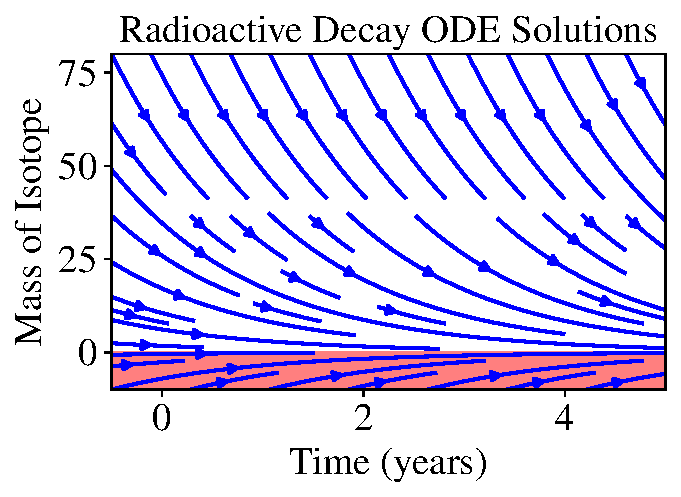
\includegraphics[width=\textwidth]{figures/radioactive_decay.pdf}
\caption{Radioactive decay ODE.}
\label{fig:radioactive_decay}
\end{subfigure}
\hfill
\begin{subfigure}[t]{0.48\textwidth}
\centering
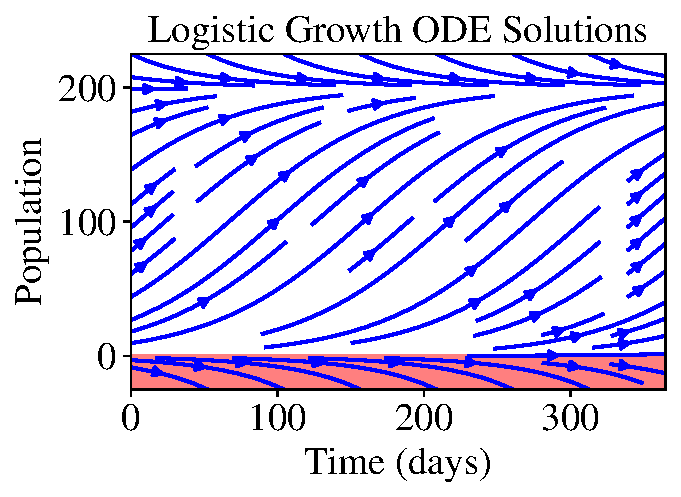
\includegraphics[width=\textwidth]{figures/logistic_growth.pdf}
\caption{Logistic growth ODE.}
\label{fig:logistic_growth}
\end{subfigure}
\caption{Phase diagrams for the two motivating homogeneous ODE models from Section~\ref{subsec:problems_with_odes}. The region below the $x$-axis (shaded red) has no physical meaning for matter isotopes. The companion Python repository on GitHub (see subsection \ref{subsec:companion_repo}) contains scripts that generate these images: \texttt{/stoch-ode/scripts/radioactive\_decay.py} and \texttt{/stoch-ode/scripts/logistic\_growth.py}. We draw both panels with \MakePhaseDiagram{} from \texttt{tools/plots/plot\_vector\_field.py} (Listing~\ref{lst:plots_vector_field}).}
\label{fig:ode_examples}
\end{figure}


Examples \ref{ex:radioactive_decay} and \ref{ex:logistic_growth} illustrate that interpreting the solutions to ODEs as describing a stochastic and discrete phenomenon requires additional intellectual framework.  System parameters and initial conditions uniquely determine solutions to suitably well-behaved ODEs, so we must account for the discrete state and stochasticity somewhere.


If the radioactive decay model is so problematic, why is it a canonical example of ODE modeling? Authors often conflate ODE solution trajectories with \textit{mean stochastic trajectories}.


\subsubsection{ODE trajectories are not mean stochastic trajectories}



Atoms are small in size and mass. A mole of atoms is a very large population ($6.023 \times 10^{23}$ atoms per mole) compared to human standards. So, the law of large numbers (LLN) and the Central Limit Theorem (CLT) both kick in when handling even relatively small masses by human standards. The LLN says behavior approaches the mean, and the CLT says behavior approaches a normal distribution, with a variance which gets tighter as sample size increases. So, the reasoning goes, a stochastic trajectory describing a large number of atoms behaves very close to the average. 

Should this not mean that the stochastic trajectories approach an ODE solution trajectory? Figure~\ref{fig:logistic_growth_mean_vs_ode} shows the logistic growth model over a short simulation window with a small sample. Over this window the dashed ODE solution and the solid stochastic mean trajectory track each other qualitatively.
Unfortunately (and contrary to popular belief) ODE solution trajectories do not generally match mean stochastic trajectories \cite{gillespie2009moment}.



\begin{figure}[htbp]
\centering
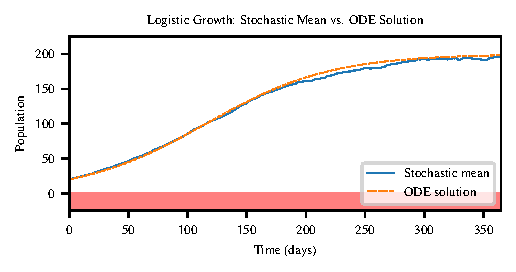
\includegraphics[width=\textwidth]{figures/logistic_growth_mean_vs_ode.pdf}
\caption{ODE solution (dashed) and Doob-Gillespie sample mean (solid), logistic growth model, $P(0) = K/2$. Short-time agreement masks qualitatively opposite long-run behavior. As usual, we shade non-physical regions red. We draw this with \PlotMeanVsOde{} from \texttt{tools/plots/plot\_mean\_vs\_ode.py} (Listing~\ref{lst:plots_mean_vs_ode}).}
\label{fig:logistic_growth_mean_vs_ode}
\end{figure}


To see why formally, note that Jensen's inequality\index{Jensen's inequality} states that, for a convex function $f$, the inequality $\mathbb{E}[f(P)] \geq f(\mathbb{E}[P])$ holds, with equality only when $f$ is affine or $P$ is almost surely constant. The death rate involves $P^2$, which is convex, so $\mathbb{E}[P^2] \geq (\mathbb{E}[P])^2$ in general. Therefore, the ODE governing $\mathbb{E}[P(t)]$ is (in general) not Equation~\ref{eqn:logistic_growth}. Modifying Equation~\ref{eqn:logistic_growth} to attain an ODE governing $\mathbb{E}[P(t)]$ requires adding higher-order terms estimated from higher-order statistical moments. We call this problem moment closure\index{moment closure} \cite{gillespie2009moment}, which lies beyond the scope of this text.

To see why more intuitively, note the long-run behaviors between exact ODE solution trajectories and stochastic realizations are qualitatively different. Consider the logistic growth model again. In the ODE, $P = K$ is a stable equilibrium: every trajectory that starts positive tends toward $P = K$ over time. The other equilibrium, $P = 0$, is unstable: a trajectory starting just above $0$ climbs toward $K$, and, as we showed above, a trajectory starting below $0$ escapes to $-\infty$ in finite time.

On the other hand, in the DG realization, stochastic trajectories do not stay at $P = K$ for long before stochastically jittering their way elsewhere. Trajectories are more likely to drift closer to $P=K$ than to drift away from $P=K$, but both are generally possible over small time intervals with strictly positive probability. Moreover, $P = 0$ is an absorbing state\index{absorbing state} for stochastic trajectories because the birth rate $rP$ and death rate $\frac{r}{K}P^2$ both vanish at $P = 0$. If the trajectory hits $0$, no further events are possible, and the population remains extinct permanently. 


Given any homogeneous ODE model whose stochastic realizations admit absorbing states, there is always a non-zero probability of a sequence of randomly sampled events which are unlucky, driving a stochastic trajectory into an absorbing state (if one exists). In fact, every step of the DG algorithm has such a probability. Generically, there is a minimum such probability $p$ for a fixed unit of simulated time $t$. We can then model which of the time intervals $[0, t)$, $[t, 2t)$, $\ldots$, $[kt, (k+1)t)$, $\ldots$ contains the extinction time as a geometric random variable. Each interval flips a coin with heads-up probability $p$, and extinction occurs in the first interval with a heads-up flip. The geometric random variable gives an upper bound on the time we expect to wait until we observe extinction. See Exercise \ref{ex:hw_bound_ext_time}.

If $P_{\texttt{ODE}}(t)$ is a solution to the ODE with a physical initial condition $P_{\texttt{ODE}}(0) > 0$, then $\underset{t \longrightarrow +\infty}{\lim} P_{\texttt{ODE}}(t) = K$. However, if $P_{\texttt{stoch}}(t)$ is a random variable describing stochastic trajectories with the same initial condition, then $\underset{t \longrightarrow +\infty}{\lim} \mathbb{E}[P_{\texttt{stoch}}(t)] = 0$. That is to say,
$$\underset{t \longrightarrow +\infty}{\lim} \mathbb{E}[P_{\texttt{stoch}}(t)] \neq \underset{t \longrightarrow +\infty}{\lim} P_{\texttt{ODE}}(t)$$ which shows that ODE solution trajectories are not mean stochastic trajectories. This argument is related to \textit{gambler's ruin}, the fact that a game with a negative expected value will eventually drive you broke, no matter your strategy. See Exercise \ref{ex:hw_gamblers_ruin}

The problem becomes more obvious when sample sizes get small and we can no longer fall back on the LLN and CLT, but the conceptual problem remains even with very large sample sizes. So, a non-trivial interpretation gap still confronts modelers after all the mathematics are said and done.







\textup{{\bf Questions for Reflection:}}
\begin{enumerate}
\item Examples~\ref{ex:radioactive_decay} and~\ref{ex:logistic_growth} are continuous-state, deterministic models, but they are modeling discrete-state, stochastic real-life systems. Provide examples of discrete-state, deterministic real-life systems?

\item Provide examples of continuous-state, stochastic real-life systems?

\item Do not fool yourself into thinking that discrete-state, deterministic processes are easy. For example, take any starting positive integer $x_0$ and, for each $i = 0, 1, 2, \ldots$, set the following.
\[x_{i+1} = \begin{cases}
\frac{x_i}{2};& x_i \textup{ is even} \\ 3x_i + 1;& x_i\textup{ is odd}
\end{cases}.\] Note that if any $x_i = 2^k$ for an integer $k > 0$, then $x_{i+k} = 1$. Investigate\footnote{Do not spend too much time on this question. Answering the question either way resolves a famously difficult, unsolved, addictive, and mysterious problem called the Collatz conjecture. The problem is sufficiently famous as to even appear in popular cinema, a dubious honor bestowed only upon the biggest wastes of time in mathematics.} whether every starting $x_0$ yields a sequence $(x_0, x_1, \ldots)$ which eventually terminates with some $x_i = 1$?
\end{enumerate}














\subsection{Structure of This Chapter}\label{subsec:structure}

The introductory chapter on the mathematical modeling process frames it as a \textit{modeling cycle} whose stages include \textit{getting a solution} and \textit{analysis and model assessment}. This chapter concentrates on those two stages. The Doob-Gillespie algorithm is our tool for getting a solution, and the parameter-sweep and sensitivity machinery supports analysis and model assessment.

\begin{itemize}
\item \textbf{Section~\ref{sec:resolving}: Resolving the Problem with Re-interpretation.} Re-interprets an ODE system as a discrete-state stochastic process. Identifies model events, derives the memoryless waiting-time distribution, and establishes the probability mass function (PMF) governing which event occurs next. The examples in this section already use integer-count units, so we require no rescaling.

\item \textbf{Section~\ref{sec:algorithm}: The Doob-Gillespie Algorithm in Detail.} Develops the full DG algorithm step by step, from the pre-processing rescaling (Step 0) through identifying events, sampling the waiting time, computing event rates, and choosing the next event.

\item \textbf{Section~\ref{sec:farming}: Doob-Gillespie Simulation Farming.} Builds DG implementations for the saline tank, logistic growth, Allee effect, and SIR models, and runs many simulations of each to estimate probabilities and summary statistics.

\item \textbf{Section~\ref{sec:visualizing_interpreting}: Visualizing and Interpreting Simulated Trajectories.} Plots individual trajectories as step graphs, aggregates many runs into heat maps, and introduces the sample statistics used to read stochastic output.

\item \textbf{Section~\ref{sec:parameter_sweep}: Parameter Space Exploration.} Introduces systematic exploration of a model across a grid of parameter values to survey qualitative behaviors and identify regions of interest.

\item \textbf{Section~\ref{sec:sensitivity_analysis}: Model Sensitivity Analysis.} Defines univariate elasticity, illustrates elasticity scoring on the logistic growth model, discusses bifurcations as qualitative regime changes, and cautions against elasticity comparisons that straddle a bifurcation point.

\item \textbf{Homework and Projects.} Homework problems reinforce the algorithmic steps. Projects are open-ended and intended as starting points for capstone or thesis investigations.

\item \textbf{Glossary.} Collects the probability and modeling terms used throughout the chapter. Consult it (Section~\ref{sec:glossary}) at the end of the chapter for any unfamiliar notation.
\end{itemize}


\subsection{Companion Python Repository on GitHub}\label{subsec:companion_repo}

 This chapter requires \texttt{Python 3.12} or later. We generate all simulations and figures in this chapter with programs and scripts written in \texttt{Python 3.12}.

To install \texttt{Python 3.12} in Windows or macOS, download and run the installer from \url{https://www.python.org/downloads/}. Otherwise, use your distribution's package manager (e.g., \texttt{sudo apt install python3} on Debian/Ubuntu). Verify the download by running \verb|python --version| in terminal. The output should begin with \texttt{Python 3.12} or higher. Our code targets \texttt{Python 3.12} or later. Readers on an older \texttt{Python} should upgrade before running the code. Our \texttt{Python} requires the \texttt{numpy} and \texttt{matplotlib} libraries. Install them via your \texttt{Python} distribution.

We host all \texttt{Python} code referenced in this chapter (scripts, simulation frameworks, and plotting utilities) at the \textbf{free} companion repository at \url{https://github.com/b-g-goodell/stoch-ode}.
\textit{Git} records the history of changes to a collection of
files. \textit{GitHub} hosts such histories and makes them publicly accessible. Students who intend to write and revise their own simulation code will find version control indispensable for keeping track of experiments and recovering from mistakes. The official tutorial at \url{https://git-scm.com/doc} is a
practical starting point. If you installed git, the following command downloads the repository into a new directory named \texttt{stoch-ode} automatically.
\begin{verbatim}
git clone https://github.com/b-g-goodell/stoch-ode
\end{verbatim}

Or, navigate to \url{https://github.com/b-g-goodell/stoch-ode}, see the repository directory structure plainly, and use \textit{Code $\to$ Download ZIP} to obtain the entire repository without Git.

The repository has the following directory structure. You can then run any script in the \texttt{scripts/} directory from within the repository directory with, for example,
\texttt{python scripts/logistic\_growth.py}. Readers who prefer interactive execution can open the scripts cell-by-cell in a \textit{Jupyter} notebook or \textit{Google Colab}.

\begin{table}[htbp]
\centering
\begin{tabular}{ll}
\hline
Directory & Contents \\
\hline
\texttt{scripts/}               & Top-level scripts for figures \\
\texttt{simulation\_frameworks/}& One framework per model \\
\texttt{tools/}                 & Plotting utilities and simulation core functions \\
\texttt{tests/}                 & Automated test suite, run with \texttt{pytest} \\
\hline
\end{tabular}
\caption{Top-level directories in the companion repository.}
\label{tab:repo_layout}
\end{table}




% Background Definitions moved to the end-of-chapter Glossary (sections/sec_11_glossary.tex).


\section{The Doob-Gillespie Interpretation}\label{sec:resolving}\index{master equation|seealso{Doob-Gillespie algorithm}}

%\textbf{Instructional Time:} 3 hours

In this section, we describe the re-interpretation of ODEs behind the DG algorithm.

Instead of a list of derivatives that change with time and state, the Doob-Gillespie algorithm\index{Doob-Gillespie algorithm} \cite{doob1942topics,doob1945markoff,gillespie1976general,gillespie1977exact} re-interprets the ODE as a \textit{master equation}, which tracks the probability of the system being in each possible discrete state at each moment in time. The master equation describes a \textit{discrete-state stochastic process}\index{simulation!stochastic} governing the system state, the distribution of events in time, and the distribution of occurring events. That is to say, we simply pseudorandomly determine the time until the next event occurs and which event occurs next.   The DG algorithm is therefore an example of a Monte Carlo algorithm, as the Monte Carlo chapter describes.

We do not need to write or handle the master equation explicitly. The DG algorithm instead generates random samples in a way which is statistically consistent with the master equation.
\begin{itemize}
\item Replace non-negative real number states (e.g.\ mass in the radioactive decay\index{radioactive decay} ODE, population in the logistic growth\index{logistic growth} ODE) with non-negative integer states (e.g.\ number of atoms, population counts, respectively).
\item Assign an independent state-change event to each rate of change in the model, using the sign to determine if the state-change event is an increase or decrease.
\item Interpret the magnitude of each term in a rate-of-change as the rate of its contributing event. For examples:
\begin{itemize}
      \item the term $- \mu M$ in the radioactive decay ODE corresponds to $E_{\texttt{decay}}$, signifying that $E_{\texttt{decay}}$ has rate $\lambda_{\texttt{decay}} = \mu M$, and
      \item the term $rP$ in the logistic growth ODE corresponds to $E_{\texttt{birth}}$ and the term $-rP/K$ corresponds to $E_{\texttt{death}}$, signifying that $E_{\texttt{birth}}$ has rate $\lambda_{\texttt{birth}} = rP$ and $E_{\texttt{death}}$ has rate $\lambda_{\texttt{death}} = rP^2/K$.
\end{itemize}
\item The rate of any event occurring in a small time interval is the sum of the rates of all events, $\lambda = \sum_{i=0}^{n-1} \lambda_i$. For example, in the logistic growth model, the rate of any event occurring is $\lambda_{\texttt{birth}} + \lambda_{\texttt{death}} = rP + rP^2/K$. Later, we show this implies a specific wait-time distribution called the \textit{exponential distribution}.
\item The probability that some event $E$ occurs in a small time interval $\left[t, t + s\right)$ is proportional to $s$ and the rate of $E$. For example, in the radioactive decay model, the probability that $E_{\texttt{decay}}$ occurs in $\left[t, t + s\right)$ is proportional to $s$ and $\lambda_{\texttt{decay}} = \mu M(t)$.
\item Given $n$ independent state-change events $E_0, E_1, \ldots, E_{n-1}$ with corresponding rates $\lambda_0, \lambda_1, \ldots, \lambda_{n-1}$, the probability that the next event to occur in a small time interval is $E_i$ (conditioned on the event that at least one of them occurs) is $\mathbb{P}\left[\text{next event is }E_i\right] = \frac{\lambda_i}{\sum_j \lambda_j}$. For example, in the logistic growth model, the probability that the next event is $E_{\texttt{birth}}$ is $\frac{rP}{rP + rP^2/K} = \frac{K}{P + K}$, and the probability that the next event is $E_{\texttt{death}}$ is $\frac{rP^2/K}{rP + rP^2/K} = \frac{P}{P + K}$.
\end{itemize}




\subsection{Examples Revisited}
\label{sec:events_in_odes}

%\textbf{Instructional Time:} 1 hour

When converting an ODE model to a model of disjoint, discrete state-change events, each population can either go up or down by some fixed amount. Their cause (whether biological, social, physical, or otherwise) uniquely identifies these events.

For Example~\ref{ex:radioactive_decay}, the radioactive decay ODE is $\frac{dM}{dt} = -\mu M$. We re-interpret the state $M(t)$ as a non-negative integer, which is a count of atoms. There is only one term, $-\mu M$, so this system describes only one independent state-change event. This term is always negative, so it corresponds to a state-change event wherein $M$ decreases, i.e.\ a decay event, say $E_{\mathrm{decay}}$. The probability that $E_{\mathrm{decay}}$ occurs in a small time interval $[t, t+s)$ is proportional to $\lambda_{\mathrm{decay}} = \left|-\mu M(t)\right| = \mu M(t)$. There is only one possible event, so the probability mass function\index{probability mass function (PMF)} is $\mathbb{P}[\textup{next event is }E_{\mathrm{decay}}] = 1$.

We can re-write the model in Example~\ref{ex:logistic_growth} as $\frac{dP}{dt} = rP - \frac{r}{K}P^2$, which has two terms, $+rP$ and $-\frac{r}{K}P^2$. The new state is $P(t)$, which we re-interpret to be a non-negative integer. The first term $rP$ corresponds to a state-change event wherein $P$ increases (a birth event\index{birth rate}, say $E_{\mathrm{birth}}$). The second term $-\frac{r}{K}P^2$ corresponds to a state-change event wherein $P$ decreases (a death event\index{death rate}, say $E_{\mathrm{death}}$).

The probability that $E_{\mathrm{birth}}$ occurs in a time interval $[t, t+s)$ is proportional to $s$ and $\lambda_{\mathrm{birth}} = \left|+rP\right| = rP$, and the probability that $E_{\mathrm{death}}$ occurs in a time interval $[t, t+s)$ is proportional to $s$ and $\lambda_{\mathrm{death}} = \left|-\frac{r}{K}P^2\right| = \frac{r}{K}P^2$. Hence, when $s$ is small the probability that $E_{\mathrm{birth}}$ or $E_{\mathrm{death}}$ occurs in $[t, t+s)$ is proportional to $s$ and $\lambda_{\mathrm{birth}}+\lambda_{\mathrm{death}}$.

The probability that the next event is $E_{\mathrm{birth}}$ is proportional to $\lambda_{\mathrm{birth}}$, and the probability that the next event is $E_{\mathrm{death}}$ is proportional to $\lambda_{\mathrm{death}}$. Hence, $\mathbb{P}[\textup{next event is }E_{\mathrm{birth}}] = \frac{\lambda_{\mathrm{birth}}}{\lambda_{\mathrm{birth}}+\lambda_{\mathrm{death}}} = \frac{rP}{rP + \frac{r}{K}P^2} = \frac{K}{K+P}$ and $\mathbb{P}[\textup{next event is }E_{\mathrm{death}}] = \frac{\lambda_{\mathrm{death}}}{\lambda_{\mathrm{birth}}+\lambda_{\mathrm{death}}} = \frac{rP/K}{rP + \frac{r}{K}P^2} = \frac{P}{K+P}$.

\needspace{5\baselineskip}
\subsection{Generating Wait-Time Between Events}\label{subsec:wait_time_prelim}


%\textbf{Instructional Time:} 1 hour



The Doob-Gillespie re-interpretation implies memorylessness. If events arrive in a memoryless way, then the amount of time already waited has no impact on how much more time remains before the next event. Knowing that a radioactive atom has existed for a certain age provides no information about how long until it decays. To discuss memorylessness, we need to discuss disjoint events, conditional probability, and independent events.
Two events $E_1, E_2$ are \textit{disjoint as sets}\index{events!disjoint} if $E_1 \cap E_2 = \emptyset$. In this case, knowledge that one occurs forbids the occurrence of the other, because the event in which both occur is the empty set. By contrast, $E_1$ and $E_2$ are \textit{independent} if knowing one occurred gives no information about whether the other occurred: formally, $\mathbb{P}[E_1 \cap E_2] = \mathbb{P}[E_1]\mathbb{P}[E_2]$.

\begin{definition}[Memoryless random variable]\label{def:memoryless}\index{memoryless property}
A random variable $T$ is \textit{memoryless} if $\mathbb{P}[T > t + s \mid T > t] = \mathbb{P}[T > s]$ for all $t, s > 0$.
\end{definition}


In a radioactive decay model with a long half-life\index{half-life}, the probability that any one atom decays in a short time interval is low. The instantaneous rate of decay at time $t$ is $\lambda(t) = \left|-\mu M(t)\right|$, which is a function of $M(t)$. If $s$ is sufficiently small, then a state-change event in $[t, t + s)$ is unlikely to occur, in which case $M(t+s) = M(t)$. Therefore, $\lambda(t+s) = \mu M(t+s) \approx \mu M(t) = \lambda(t)$. Memorylessness means an event has approximately constant probability of occurrence over short intervals of time.

\begin{example}\label{ex:exponential_memoryless}
\textbf{The Exponential Distribution is Memoryless.}
Let $T \sim \text{Exp}(\lambda)$ be an \textit{exponentially distributed random variable}\index{distribution!exponential}. Then $T$ is memoryless. $T$ has cumulative distribution function\index{cumulative distribution function (CDF)} $1 - e^{-\lambda t} = \mathbb{P}[T \leq t]$ (equivalently, $e^{-\lambda t} = \mathbb{P}[T > t]$). Recall the conditional probability of event $A$ conditioned on event $B$ as $\mathbb{P}[A \mid B] = \mathbb{P}[A \cap B]/\mathbb{P}[B]$. So $\mathbb{P}[T > t + s \mid T > t] = \tfrac{\mathbb{P}[T > t + s\text{ and } T > t]}{\mathbb{P}[T > t]}$. For $t, s \geq 0$, $T > t + s$ implies $T > t$, reducing to $\frac{\mathbb{P}[T > t + s]}{\mathbb{P}[T > t]} = \frac{e^{-\lambda (t + s)}}{e^{-\lambda t}} = e^{-\lambda s} = \mathbb{P}[T > s]$.
\end{example}

It turns out that the only continuous memoryless random variable is the \textit{exponential random variable} (see \cite{grimmett2020probability}). Inter-event wait times in the Doob-Gillespie algorithm must be memoryless, so simulating a continuous-time ODE requires wait times sampled from an exponential distribution.
Wait times follow the exponential distribution, so we sample them exactly using the inverse CDF method\index{inverse CDF method}. Recall the cumulative distribution function for a random variable $X$ is the function $F(x) = \mathbb{P}\left[X \leq x\right]$. The inverse CDF method samples a random variable $X$ with CDF $F$ by sampling $U \sim \text{Uniform}(0, 1)$ and returning $F^{-1}(U)$. For an exponential random variable with parameter $\lambda$, the CDF is $F(t) = 1 - e^{-\lambda t}$, so the inverse CDF is $F^{-1}(U) = -\frac{1}{\lambda}\ln(1-U)$. See \cite{grimmett2020probability} for more details on the exponential distribution and the inverse CDF method.

The exponential distribution has a single parameter, $\lambda > 0$, which equals the total rate of all events. The Doob-Gillespie algorithm models the time until the next event as an exponential random variable and uses the sum of the rate of change magnitudes as $\lambda$. We call a process in which events arrive independently at a constant rate $\lambda$ a \textit{Poisson process}\index{Poisson process}. Every time the DG algorithm changes the simulated state, the rates of change and therefore $\lambda$ change, so the process is not properly a Poisson process.

In the case of Example~\ref{ex:radioactive_decay}, the time until the next event occurs is exponentially distributed with parameter $\lambda = \mu M(t)$. In the case of Example~\ref{ex:logistic_growth}, the time until the next event occurs is also exponentially distributed, but with parameter $\lambda = rP(t)\left(1 + \frac{1}{K}P(t)\right)$. The total event rate has a factor $1 + P/K$, not the $1 - P/K$ of the ODE, because $\lambda$ sums the birth and death rate magnitudes $rP$ and $rP^2/K$, whereas the ODE takes their difference.

{\bf Questions for Reflection:}
\begin{enumerate}
\item Radioactive decay is a memoryless process. Interpret memorylessness in the context of the radioactive decay model.

\item In the logistic growth model, the total event rate is $\lambda = rP(1 + P/K)$. As $P$ grows from $1$ to $K$, by what factor does $\lambda$ increase? What does this imply for the expected wait time between events and for simulation runtime at large populations?

\item The DG algorithm samples a fresh wait time from the exponential distribution after every event. A student proposes a shortcut: sample one large exponential wait time at the start and ``spend'' it across multiple events. Explain why this shortcut is incorrect.

\end{enumerate}


\subsection{Determining Which Event Occurs Next}\label{subsec:which_event}


%\textbf{Instructional Time:} 1 hour

If the next event to occur is $E_i$ with a probability proportional to $\lambda_i$, and the only possible next events are $E_0, E_1, \ldots, E_{n-1}$, then the probability that the next event is $E_i$ is exactly $\frac{\lambda_i}{\sum_j \lambda_j}$. This value follows from normalization: the probabilities sum to $1$, and each is proportional to its rate.

\begin{example}\label{ex:normalize_pmf}
\textbf{Normalizing a PMF from Event Rates.}
For example, presume we have events $E_0, E_1, E_2$ with rates $\lambda_0, \lambda_1, \lambda_2$. Further presume that $\lambda_1 = 2\lambda_0$ and $\lambda_2 = 3 \lambda_0$. Let $p_i$ be the probability that the next event is $E_i$ for each $i=0,1,2$. These probabilities are proportional to their events' rates, so $p_0 = c \lambda_0$, $p_1 = c \lambda_1 = 2c\lambda_0$, and $p_2 = c \lambda_2 = 3c\lambda_0$. The probabilities sum to $1$, so $p_0 + p_1 + p_2 = 6c\lambda_0 = 1$. Thus, $c = \frac{1}{6\lambda_0}$, so $p_0 = \frac{1}{6}$, $p_1 = \frac{1}{3}$, and $p_2 = \frac{1}{2}$.
\end{example}

In Example~\ref{ex:radioactive_decay}, there is only one event, the death event, which must occur with probability $1$. In Example~\ref{ex:logistic_growth}, there are two events, birth and death; normalizing their rates $rP$ and $\frac{r}{K}P^2$ as above gives next-event probabilities $\frac{K}{P+K}$ for a birth and $\frac{P}{P+K}$ for a death.

\textup{{\bf Questions for Reflection:}}
\begin{enumerate}
\item Geometric random variables are also memoryless. They are discrete and take on positive integer values $1$, $2$, $3$, $\ldots$. They have one parameter, $0 < p \leq 1$, and represent the number of flips of a biased coin with bias $p$ until the first heads-up flip occurs. Postulate why we should not use geometric random variables to increment time while simulating an ODE.


\item Explain why simulating a trajectory of an asteroid headed for earth is not a good task for the Doob-Gillespie algorithm.

\item A reaction network has one fast event with rate $\lambda_1 = 10^6$ and one slow event with rate $\lambda_2 = 1$. Approximately what fraction of simulated events are the fast event? Discuss the implications when the scientists want to observe the slow event.
\end{enumerate}


\section{The Doob-Gillespie Algorithm in Detail with Examples}\label{sec:algorithm}

%\textbf{Instructional Hours:} 12-18 hours

The Doob-Gillespie algorithm uses the ODE parameters and initial conditions to generate a \textit{stochastic trajectory}\index{trajectory!stochastic}. The word \textit{stochastic} means \textit{random}. Unlike ODE solutions, which system parameters and initial conditions fully determine, a stochastic trajectory is one possible random realization of the system evolution. Concretely, a stochastic trajectory is a sequence of time-state tuples $(t_0, {\tt state}_0), (t_1, {\tt state}_1), (t_2, {\tt state}_2), \ldots$, where $(t_i, {\tt state}_i)$ records the time and system state immediately after the $i^{th}$ state-change event occurs. The algorithm proceeds as follows. Steps 0 and 1 are pre-processing steps: run them once before any simulation begins. Step 2 initializes the simulation bookkeeping. Steps 3 and forward constitute the main loop, which repeats while the clock $t$ remains below the simulation run time $T$.
\begin{enumerate}
\item[\textbf{Step 0.}] (Pre-processing.) Scale\index{rescaling} and/or re-parameterize\index{re-parameterization} the system so that the state variable counts discrete individuals. Perform this step once, before the simulation loop begins.
\item[\textbf{Step 1.}] (Pre-processing.) Identify all the state-change events $\left\{E_i\right\}_i$ and their effects on the state $\left\{\delta_i\right\}_i$.
\item[\textbf{Step 2.}] (Initial bookkeeping.) Set $t = 0$, set the state to the initial conditions, and record the time and state.
\item[\textbf{Step 3.}] Use the current state to compute the rate $\lambda_i$ of each event.
\item[\textbf{Step 4.}] Compute the total rate $\lambda = \sum_i \lambda_i$ and the PMF $p_i = \lambda_i/\lambda$.
\item[\textbf{Step 5.}]   If $\lambda = 0$, terminate. 
\item[\textbf{Step 6.}] Sample $U \sim \text{Uniform}(0,1]$ and compute $\Delta t \sim Exp(\lambda)$ by setting $\Delta t = -\ln(U)/\lambda$.
\item[\textbf{Step 7.}] Sample $W \sim \text{Uniform}(0,1]$, compute the index $j$ of the next event $E_j$ from the PMF $\left\{p_i\right\}_i$ by setting $j = \min\left\{k \middle| \sum_{i \leq k} p_i \geq W\right\}$, and look up the state-change event $\delta_j$.
\item[\textbf{Step 8.}] Update the clock $t \leftarrow t + \Delta t$, the state $\texttt{state} \leftarrow \texttt{state} + \delta_j$, record the new time and state, and, if $t < T$, go back to step 3.
\end{enumerate}

The algorithm calls five subroutines: $\textsf{MakeDeltaStates}$ tabulates the state changes once in Step 1, and the main loop then calls $\textsf{MakeRates}$ to evaluate the event rates, $\textsf{RatesToPmf}$ to form the PMF and total rate, $\textsf{RateToDeltaTime}$ to sample the waiting time, and $\textsf{PmfToEventIndex}$ to select the next event.
Note that computing rates, and looking up the state-change event after sampling an index $j$, both depend on the ODE model.
All else is the same for every ODE model, and we implement it generically. We index the $n$ events from $0$ to $n-1$ throughout, matching the companion \texttt{Python}.

We assemble these subroutines into the full algorithm. Figure~\ref{fig:dg_algorithm} presents it symbolically, the numbered steps above explain it, and each line of the figure shows its step. Figures~\ref{fig:dg_subroutines_a} and~\ref{fig:dg_subroutines_b} collect the pseudocode for the five subroutines it calls. Listing~\ref{lst:dg_algorithm_python_template} gives the \texttt{Python 3.12} implementation, a template that follows the same steps line for line. It diverges from the pseudocode only at Step 5: rather than breaking out of the loop, it returns the trajectory as soon as \RatesToPmf{} yields a total rate of zero.

\begin{figure}[htbp]
\centering
{\footnotesize
\fbox{\procedure{Doob-Gillespie Algorithm $\textsf{DG}(T,\, x_0,\, \theta) \to \textsf{traj}$:}{
\pcind (\delta_j)_{j=1}^{N} \leftarrow \textsf{MakeDeltaStates}(\theta)\,; \pccomment{\text{Step 1}}\\
\pcind t \leftarrow 0 \,;\; x \leftarrow x_0 \,;\; \textsf{traj} \leftarrow [(0,\, x_0)]\,; \pccomment{\text{Step 2}}\\
\pcind \pcwhile t < T \pcdo \\
\pcind\pcind \vec{\lambda} \leftarrow \textsf{MakeRates}(x,\, \theta)\,; \pccomment{\text{Step 3}} \\
\pcind\pcind (\vec{p},\, \lambda) \leftarrow \textsf{RatesToPmf}(\vec{\lambda})\,; \pccomment{\text{Step 4}}\\
\pcind\pcind\pcif \lambda = 0 \pcthen \textbf{break}\,; \pccomment{\text{Step 5}} \\
\pcind\pcind \Delta t \leftarrow \textsf{RateToDeltaTime}(\lambda)\,; \pccomment{\text{Step 6}} \\
\pcind\pcind j \leftarrow \textsf{PmfToEventIndex}(\vec{p})\,; \pccomment{\text{Step 7}} \\
\pcind\pcind t \leftarrow t + \Delta t \,;\; x \leftarrow x + \delta_j \,; \pccomment{\text{Step 8}} \\
\pcind\pcind \textsf{traj} \leftarrow \textsf{append}\left(\textsf{traj}, [(t,\, x)]\right)\,; \\
\pcind\pcendwhile\\
\pcind \pcreturn \textsf{traj}
}}}
\caption{Doob-Gillespie algorithm, Steps 1 to 8. Here $T$ is the simulation run time, $x_0$ is the initial state, $\theta$ is the parameter vector, $\vec{\lambda}$ is the event-rate vector, $\vec{p}$ is the event PMF, and $(\delta_j)_{j=1}^{N}$ are the state changes from the $N$ events. The subroutines $\textsf{MakeDeltaStates}$, $\textsf{MakeRates}$, $\textsf{RatesToPmf}$, $\textsf{RateToDeltaTime}$, and $\textsf{PmfToEventIndex}$ appear in Figures~\ref{fig:dg_subroutines_a} and~\ref{fig:dg_subroutines_b}. The list $\textsf{traj}$ accumulates the $(t, x)$ pairs.}
\label{fig:dg_algorithm}
\end{figure}

\lstinputlisting[float=htbp,
language=Python,
numbers=none,
caption={Python template for DG simulations. Compare to Figure~\ref{fig:dg_algorithm}. See \texttt{/stoch-ode/simulation\_frameworks/framework\_template.py} in the Python repository.},
label={lst:dg_algorithm_python_template}]{../simulation_frameworks/framework_template.py}

\begin{figure}[htbp]
\centering
{\footnotesize
\adjustbox{valign=t}{\fbox{\procedure{$\textsf{MakeRates}(x,\, \theta) \to \vec{\lambda}$:}{
\pcind \pcforeach \text{event } E_i \pcdo \\
\pcind\pcind \lambda_i \leftarrow \lambda_i(x;\, \theta)\,; \\
\pcind \pcendforeach \\
\pcind \pcreturn \vec{\lambda} = (\lambda_0, \ldots, \lambda_{n-1})
}}}\hfill
\adjustbox{valign=t}{\fbox{\procedure{$\textsf{RateToDeltaTime}(\lambda) \to \Delta t$:}{
\pcind \pcif \lambda \leq 0 \pcthen \textbf{error}\,; \\
\pcind V \sim \mathrm{Uniform}(0,1]\,; \\
\pcind \pcreturn -\ln(V)/\lambda
}}}\hfill
\adjustbox{valign=t}{\fbox{\procedure{$\textsf{MakeDeltaStates}(\theta) \to (\delta_j)_j$:}{
\pcind \pcreturn (\delta_j)_{j=1}^{N}
}}}\par}
\caption{Three Doob-Gillespie subroutines, each in its own box. $\textsf{MakeRates}$ evaluates the rate $\lambda_i$ of each event $E_i$ at the current state $x$ under parameters $\theta$. $\textsf{RateToDeltaTime}$ samples an exponential waiting time $\Delta t$ with rate parameter $\lambda$ by inverse-CDF sampling, and \RateToDeltaTime{} implements it generically. $\textsf{MakeDeltaStates}$ returns the vector $(\delta_j)_{j=1}^{N}$ of state changes for the $N$ events, which we tabulate once in Step 1. The bodies of $\textsf{MakeRates}$ and $\textsf{MakeDeltaStates}$ are model-specific: each model supplies its own, for example \MakeLogisticRates{} and \MakeLogisticDeltaStates.}
\label{fig:dg_subroutines_a}
\end{figure}

\begin{figure}[htbp]
\centering
{\footnotesize
\adjustbox{valign=t}{\fbox{\procedure{$\textsf{RatesToPmf}(\vec{\lambda}) \to (\vec{p},\, \lambda)$:}{
\pcind \pcif \lambda_i < 0 \;\text{for any}\; i \pcthen \textbf{error}\,; \\
\pcind \lambda \leftarrow \textstyle\sum_i \lambda_i\,; \\
\pcind \pcif \lambda = 0 \pcthen \pcreturn \bot\,; \\
\pcind \pcforeach i \in \{0, \ldots, n-1\} \pcdo \\
\pcind\pcind p_i \leftarrow \lambda_i/\lambda\,; \\
\pcind \pcendforeach \\
\pcind p_{n-1} \leftarrow 1 - \textstyle\sum_{i < n-1} p_i\,; \\
\pcind \pcreturn (\vec{p},\, \lambda)
}}}\hfill
\adjustbox{valign=t}{\fbox{\procedure{$\textsf{PmfToEventIndex}(\vec{p}) \to j$:}{
\pcind \pcif p_i \notin [0,1] \;\text{for any}\; i \pcthen \textbf{error}\,; \\
\pcind \pcif \left\lvert \textstyle\sum_i p_i - 1 \right\rvert > \varepsilon \pcthen \textbf{error}\,; \\
\pcind U \sim \mathrm{Uniform}(0,1]\,; \\
\pcind j \leftarrow 0 \,;\; c \leftarrow p_0\,; \\
\pcind \pcwhile (c < U \;\textbf{or}\; p_j = 0) \;\textbf{and}\; j < n-1 \pcdo \\
\pcind\pcind j \leftarrow j + 1 \,;\; c \leftarrow c + p_j\,; \\
\pcind \pcendwhile \\
\pcind \pcreturn j
}}}\par}
\caption{Two generic Doob-Gillespie subroutines, each in its own box. $\textsf{RatesToPmf}$ rejects a negative rate, sums the total rate $\lambda$, and returns the PMF $\vec{p}$ with $p_i = \lambda_i/\lambda$. Setting $p_n$ by subtraction forces $\sum_i p_i = 1$. A zero total rate signals an absorbing state, so it returns $\lambda = 0$ for the caller to terminate (Step 5). $\textsf{PmfToEventIndex}$ samples $U \sim \mathrm{Uniform}(0,1]$ and returns the index $j$ of the selected event by a cumulative scan of $\vec{p}$, with the tolerance $\varepsilon$ guarding the normalization check. Both are the same for every model, and \RatesToPmf{} and \PmfToEventIndex{} implement them.}
\label{fig:dg_subroutines_b}
\end{figure}

$\textsf{MakeRates}$ loops over the events $E_0, \ldots, E_{n-1}$, evaluates each rate $\lambda_i$ at the current state, and returns the rate vector $\vec{\lambda}$. $\textsf{RateToDeltaTime}$ rejects a non-positive total rate, samples $V$ uniformly from $(0,1]$, and returns the waiting time $-\ln(V)/\lambda$ (Section~\ref{subsec:wait_time} derives this inverse-CDF formula). $\textsf{MakeDeltaStates}$ returns the vector $(\delta_j)_{j=1}^{N}$ of state changes for the $N$ events, which we tabulate once in Step 1. $\textsf{RatesToPmf}$ rejects any negative rate, sums the total rate $\lambda$, and returns a distinct failure symbol $\bot$ when $\lambda = 0$ to flag an absorbing state for the caller. Otherwise it sets each $p_i = \lambda_i/\lambda$, replaces the last entry by $1 - \sum_{i < n-1} p_i$ so the probabilities sum to one despite rounding, and returns the pair $(\vec{p}, \lambda)$. $\textsf{PmfToEventIndex}$ rejects a $\vec{p}$ with an entry outside $[0,1]$ or a sum more than $\varepsilon$ from one, samples $U$ uniformly from $(0,1]$, initializes the index $j$ and the cumulative sum $c$ at the first probability, advances $j$ while $c < U$ or the current probability is zero and while $j$ stays below $n-1$, and returns the selected index $j$ (Section~\ref{subsubsec:construct_pmf} develops the cumulative scan).

Three of these subroutines are model-independent and live in the companion code's simulation core, \texttt{tools/simcore.py}. In Figure~\ref{fig:dg_subroutines_a}, $\textsf{RateToDeltaTime}$ inputs a total rate $\lambda$ and outputs an exponential waiting time $\Delta t$ by inverse-CDF sampling. Listing~\ref{lst:framework_rate_to_delta_time} gives its \texttt{Python} implementation \RateToDeltaTime{}, which realizes the sample $V \sim \mathrm{Uniform}(0,1]$ as \texttt{1.0 - random()} because \texttt{random()} returns a value in $[0,1)$. In Figure~\ref{fig:dg_subroutines_b}, $\textsf{RatesToPmf}$ inputs the rate vector $\vec{\lambda}$ and outputs the PMF $\vec{p}$ and total rate $\lambda$, and $\textsf{PmfToEventIndex}$ inputs $\vec{p}$ and outputs the index $j$ of the next event. Listing~\ref{lst:framework_dg_core} gives their \texttt{Python} implementations \RatesToPmf{} and \PmfToEventIndex{}. The \texttt{Python} diverges from the pseudocode in two ways: \RatesToPmf{} also rejects an empty rate vector, and it clamps the normalized last entry with \texttt{max(0.0, ...)} so a small negative rounding error becomes zero rather than a negative probability.

\lstinputlisting[float=htbp, language=Python, numbers=none, linerange={34-38}, caption={The generic \texttt{Python} waiting-time subroutine \RateToDeltaTime{}, paired with the pseudocode $\textsf{RateToDeltaTime}$ of Figure~\ref{fig:dg_subroutines_a}.}, label={lst:framework_rate_to_delta_time}]{../tools/simcore.py}

\lstinputlisting[float=htbp, language=Python, numbers=none, linerange={7-31}, caption={The generic \texttt{Python} subroutines \RatesToPmf{} and \PmfToEventIndex{}, paired with the pseudocode of Figure~\ref{fig:dg_subroutines_b}.}, label={lst:framework_dg_core}]{../tools/simcore.py}

Section~\ref{sec:resolving} introduced three of the four probabilistic concepts the algorithm requires. Each corresponds to a step in the list above. Section~\ref{sec:events_in_odes} introduced the identification of distinct model events and their rate functions from the ODE (Step 1), which the algorithm evaluates at runtime in Step 3. Section~\ref{sec:resolving}'s subsection on wait-time developed the memoryless property of inter-event times and showed that those times are exponentially distributed, with the total rate $\lambda$ as the distribution parameter (Step 6). The subsection on which event occurs next showed that the probability of each event is proportional to its rate, yielding the PMF $p_i = \lambda_i/\lambda$ (Step 4). Section~\ref{sec:resolving} does not develop Step 0: the examples there (radioactive decay, logistic growth) already use integer-count units and require no rescaling.

\FloatBarrier

\subsection{Re-Scaling and Re-Parameterizing to Integer Counts}\label{subsec:alg_rescaling}

%\textbf{Instructional Time:} 2 hours

The DG algorithm\index{Doob-Gillespie algorithm} simulates discrete jumps in state by $\pm 1$ at a time, so we scale\index{rescaling} the ODE system such that the state variable discretely counts individuals (such as molecules or organisms). This requires a change of variables.\index{change of variables}


\begin{example}\label{ex:radioactive_decay_units}
Take a fictional isotope with measured half-life $\tau = 5.00 \times 10^{3}\,\mathrm{s}$ and initial sample mass $M_0 = 2.5\,\mathrm{lb}$. Your boss demands a simulation running in years and kilograms. The per-second decay rate is
\[
  \mu = \frac{\ln 2}{\tau}
      = \frac{\ln 2}{5.00 \times 10^{3}\,\mathrm{s}}
      \approx 1.386 \times 10^{-4}\,\mathrm{s}^{-1}.
\]
The relevant conversion factors are
\[
  1\,\mathrm{lb} = 0.4536\,\mathrm{kg},
  \qquad
  1\,\mathrm{yr} = 3.156 \times 10^{7}\,\mathrm{s}.
\]
Whereas $M_0$ is measured in pounds and $\tau$ is measured in seconds, let $\widetilde{M}$ denote mass in kilograms and $T$ time in years.
Substituting $M = \widetilde{M}/0.4536$ and $t = T \cdot 3.156 \times 10^{7}$
into $\frac{dM}{dt} = -\mu M$ gives
\[
  \frac{1}{0.4536} \cdot \frac{1}{3.156 \times 10^{7}}
  \frac{d\widetilde{M}}{dT}
  =
  -\mu \cdot \frac{\widetilde{M}}{0.4536}.
\]
The factor $1/0.4536$ appears on both sides and cancels, leaving
\[
  \frac{d\widetilde{M}}{dT}
  = -\underbrace{\bigl(\mu \cdot 3.156 \times 10^{7}\bigr)}_{\displaystyle\widetilde{\mu}}\,
  \widetilde{M}
  \approx -4374\,\mathrm{yr}^{-1} \cdot \widetilde{M}.
\]
The initial condition converts as
$\widetilde{M}_0 = 2.5 \times 0.4536 \approx 1.134\,\mathrm{kg}$.
Because the ODE is linear in mass, and with the same unit on both sides,
the mass conversion factor cancels. Only the time unit requires a numerical
change to $\mu$.
\end{example}

\begin{example}\label{ex:saline_tank}
\textbf{Saline Tank Model.} A nanomachinery manufacturer has made a motivating observation for mathematical modeling: a sensitive manufacturing process requires a saline solution with precise quantities of salt to avoid failure. The manufacturer articulates the problem in the following way.
\begin{itemize}
\item If too many or too few NaCl molecules (really, Na-Cl ion pairs in aqueous solution) enter the mixing tank, the industrial process fails, so we must model the absolute number of molecules.
\item A tank with $V$ units of volume, two inlet pipes, and one outlet pipe holds the well-mixed saline solution.
\item One inlet pipe brings in distilled water at rate $a$ units of volume per unit of time.
\item Another inlet pipe brings in a saline solution at $b$ units of volume per unit of time with concentration $c$ units of mass per unit of volume.
\item The outlet pipe drains $a+b$ units of volume of the well-mixed solution per unit of time.
\end{itemize}

We formulate an ODE governing the salt concentration in the tank as $\frac{dX}{dt} = \frac{bc}{V} - \frac{a+b}{V}X$. The saline inlet adds $bc$ units of mass per unit time to a tank of volume $V$, so the concentration increases at rate $bc/V$. The outlet removes the well-mixed solution at total volumetric rate $a+b$, diluting the concentration at rate $(a+b)X/V$.

The number of molecules $M$ times mass per molecule $m$ is the total mass, and the total mass per volume $V$ is the concentration. Let $X = mM/V$, where $M$ is the number of NaCl molecules in the tank, $m$ is the mass of each molecule in the same mass units as $X$ and $c$, and $V$ is the volume. Taking the derivative of both sides of $X = mM/V$ gives us the following.
\begin{align}
\frac{m}{V}M =& X \notag \\
\frac{d}{dt} \frac{m}{V}M =& \frac{d}{dt} X \notag \\
\frac{m}{V} \frac{dM}{dt} =& \frac{dX}{dt} \notag \\
\frac{m}{V} \frac{dM}{dt} =& \frac{bc}{V} - \frac{a+b}{V}X \notag \\
\frac{m}{V} \frac{dM}{dt} =& \frac{bc}{V} - \frac{a+b}{V} \frac{mM}{V} \notag \\
m \frac{dM}{dt} =& bc - m\frac{a+b}{V}M \notag \\
\frac{dM}{dt} =& \frac{bc}{m} - \frac{a+b}{V}M \label{eqn:saline_tank}
\end{align} Now the evolution of $M$ takes place on the scale of individual molecules. This process works regardless of the underlying parameters $a$, $b$, $c$, $m$, and $V$.

\end{example}

Sometimes a change of variables requires changing time as in Example~\ref{ex:radioactive_decay_units} or Homework Problem~\ref{ex:hw_brusselator_transform}
Sometimes, different system parameters are given in different unit systems (e.g., a volume measured in liters but a flow rate in gallons per second).
Example~\ref{ex:saline_tank_with_repar} illustrates unit-conversion with mixed units.
When mixed units are on the table, we can get real weird with it.



\begin{example}\label{ex:saline_tank_with_repar}
\textbf{Saline Tank Model with Mixed Units.}
Mixed units occur frequently during meta-analyses comparing data from multiple sources, measured in units distinct to each source. Convert all variables to compatible unit systems before applying the methods in this chapter.

Consider the tank in the previous problem, except the parameters $V$, $a$, $b$, $c$, and $m$ appear in inconsistent units: say $V$ is in liters, $a$ and $b$ are both in cubic light-years per year, $c$ is in kilograms per gallon, and $m$ is in pounds. Because the units are inconsistent, the concentration of salt in the tank no longer obeys the differential equation $\frac{dX}{dt} = \frac{bc}{V} - \frac{a+b}{V}X$ and the mass does not obey $\frac{dM}{dt} = \frac{bc}{m} - \frac{a+b}{V}M$. The term $bc/V$ adds a quantity with units $\frac{(\text{light-year})^3}{\text{year}} \cdot \frac{\text{kg}}{\text{gal}} \cdot \frac{1}{\text{liter}}$, which one cannot add to $\frac{a+b}{V}X$, measured in different units. Do not perform arithmetic on quantities with mismatched units.


Reformulate the model using liters, hours, and grams, with new parameters $\widetilde{V}$, $\widetilde{a}$, $\widetilde{b}$, $\widetilde{c}$, and $\widetilde{m}$.
\begin{itemize}
\item The parameter $V$ is already in liters, so set $\widetilde{V} = V$.
\item The parameters $a$ and $b$ are both in cubic light-years per year,
$\frac{(\textup{light year})^3}{year}$,
which is a measure of volume over time. We need these parameters in liters per hour,
$\frac{\textup{liter}}{\textup{hour}}$
. Readers should verify for themselves that there are $9.667\times 10^{46} \frac{\textup{liter}}{\textup{hour}}$ in
$1 \frac{(\textup{light year})^3}{\textup{year}}$.
So, $a \frac{(\textup{light year})^3}{\textup{year}} =  9.667 a \times 10^{46} \frac{\textup{liter}}{\textup{hour}}$. Set $\widetilde{a} = 9.667a \times 10^{46} \frac{\textup{liter}}{\textup{hour}}$ and, similarly, $\widetilde{b} = 9.667b\times 10^{46} \frac{\textup{liter}}{\textup{hour}}$.
\item The parameter $c$ is in kilograms per gallon $\frac{\textup{kg}}{\textup{gal}}$. There are $264.2$ grams per liter $\frac{\textup{gram}}{\textup{liter}}$ in $1 \frac{\textup{kilogram}}{\textup{gallon}}$. So, set $\widetilde{c} = 264.2c \frac{\textup{gram}}{\textup{liter}}$.
\item The parameter $m$ is in pounds $\textup{lbs}$ per molecule. There are $453.6\textup{ grams}$ per $1\textup{ lbs}$. So, set $\widetilde{m} = 453.6m \frac{\textup{grams}}{\textup{molecule}}$.
\end{itemize} Now the parameters $\widetilde{V}$, $\widetilde{a}$, $\widetilde{b}$, $\widetilde{c}$, and $\widetilde{m}$ can replace $V, a, b, c, m$ as in Example~\ref{ex:saline_tank}, giving $\frac{dM}{dt} = \frac{\widetilde{b}\widetilde{c}}{\widetilde{m}} - \frac{\widetilde{a}+\widetilde{b}}{\widetilde{V}}M$. The equation has the same algebraic form as before. Only the numerical values of the parameters have changed for consistency in units.



\end{example}

\textup{{\bf Questions for Reflection:}}
\begin{enumerate}
\item In Example~\ref{ex:radioactive_decay_units}, the factor $1/0.4536$ appeared on both sides of the rescaled ODE and canceled. Explain in general why a multiplicative rescaling of the state variable does not change the qualitative dynamics of a linear ODE, but does change the numerical value of the rate parameter.

\item The saline tank model introduces the mass per molecule $m$ to convert mass to molecule count. As $m \to 0$ with total mass held fixed, the molecule count grows without bound. Describe what happens to the DG simulation in this limit and why the continuous ODE remains a valid description.

\item A colleague proposes running a DG simulation with parameters measured in inconsistent units, arguing that the results will look reasonable enough. Construct a specific counterexample using the saline tank model to show that unit inconsistency produces a numerically incorrect simulation, and identify the symptom a researcher would observe.
\end{enumerate}

\subsection{Identifying Events and Their State Changes}\label{subsec:events}\index{state-change event}

%\textbf{Instructional Time:} 1 hour

The next step in the Doob-Gillespie\index{Doob-Gillespie algorithm} framework is to identify the state-change events and their effects. Each independent model event corresponds to a \textit{distinct} analytic term in a reduced representation of the ODE (see Section~\ref{sec:resolving}). Each term with its own sign and functional dependence corresponds to one independent event, so count the distinct terms, not the equations.

For example, $\frac{dY}{dt} = \lambda Y + \mu Y^2 = \frac{\lambda}{2}Y + \frac{\lambda}{2}Y + \frac{\mu}{3}Y^2 + \frac{\mu}{3}Y^2 + \frac{\mu}{3}Y^2$, where the former is the reduced representation. This ODE has two distinct terms, $\lambda Y$ and $\mu Y^2$.

See Section~\ref{sec:events_in_odes} for model events in Examples~\ref{ex:radioactive_decay} and~\ref{ex:logistic_growth}. In Example~\ref{ex:saline_tank}, two events appear: salt entering or leaving the tank.\index{model!saline tank} The term $+\frac{bc}{m}$ corresponds to the event in which a salt molecule arrives via the inlet pipe, increasing $M$ by $1$. The term $-\frac{a+b}{V} M$ corresponds to the event in which a salt molecule leaves via the outlet pipe, decreasing $M$ by $1$. The salt-arrival rate $\frac{bc}{m}$ does not depend on $M$, but the departure rate does. Here are fourth and fifth examples.

\begin{example}
\label{ex:allee}
\textbf{Allee Effect Model.}\index{Allee effect}
Let $K > L > 0$ and $r > 0$. Allee \cite{allee1931animal} showed that many populations exhibit reduced per-capita growth rates at low density, a phenomenon researchers now call the Allee effect.
A long time in the future, in our own galaxy, a certain organism produces a magic spice which runs the entire galactic economy.
In addition to the usual carrying capacity imposed by a natural environment with finite resources, Imperial Planetologists have discovered that the species is subject to the \textit{Allee effect}.
The emperor wishes to determine the probability that a colony of this species goes extinct.
Imperial Planetologists refine the logistic model of Equation~\ref{eqn:logistic_growth} to include the Allee effect during model formulation.
In the logistic model, the population size modulates the \textit{effective} per-capita birth rate with respect to a carrying capacity $K > 0$, giving birth rate $r(1-\frac{P}{K})$.
The Allee model applies the same idea twice, modulating the effective birth rate according to both a \textit{cooperation threshold}\index{cooperation threshold} and the carrying capacity\index{carrying capacity} $K$.
\begin{equation}
\label{eqn:allee}
\frac{dP}{dt} = -r P(1-\frac{P}{L})(1- \frac{P}{K})
\end{equation}
Each term in $\frac{dP}{dt}$ needs units $\frac{\textup{individual}}{\textup{time}}$, so $r$ must be in units $(\textup{time})^{-1}$, and both $L$, $K$ must be in units $\textup{individuals}$. The state is $P(t)$, a non-negative real number. The factor $(1 - P/L)(1 - P/K)$ is dimensionless and modifies the per-capita growth rate, analogous to the factor $(1 - P/K)$ in the logistic growth model. $P = L$ and $P = K$ are equilibria (substituting either into $\frac{dP}{dt}$ gives $0$). The equilibrium $P = L$ is \emph{locally unstable}\index{equilibrium!unstable}: small perturbations away from $L$ grow rather than shrink, so the population drifts away from $L$. The equilibrium $P = K$ is \emph{locally stable}\index{equilibrium!stable}: the system corrects small perturbations, so the population returns to $K$.
Expand the right-hand side of $\frac{dP}{dt}$ like so.
\[
-rP\left(1 - \tfrac{P}{L} - \tfrac{P}{K} + \tfrac{P^2}{LK}\right)
= -rP + \frac{r}{L}P^2 + \frac{r}{K}P^2 - \frac{r}{LK}P^3.
\]
This yields four terms, hence four state-change events:
\begin{itemize}
\item a natural death event, decreasing $P$ by $1$, occurring with rate $rP$;
\item a death event which would not have occurred without competition, decreasing $P$ by $1$, occurring with rate $\frac{r}{LK}P^3$;
\item a birth event related to the carrying capacity, increasing $P$ by $1$, occurring with rate $\frac{r}{K}P^2$; and
\item a birth event related to the cooperation threshold, increasing $P$ by $1$, occurring with rate $\frac{r}{L}P^2$.
\end{itemize}

In the (continuous-state) ODE, if $\frac{dP}{dt} = 0$, then $P = 0$, $P = L$, or $P = K$. These are the equilibria.
However, the total rate of all events is $\lambda = rP + \frac{r}{L}P^2 + \frac{r}{K}P^2 + \frac{r}{LK}P^3 = rP(1 + \frac{P}{L})(1 + \frac{P}{K})$.
So, the only equilibrium which has a zero total rate is $P = 0$.
At $P = K$ or $P = L$, the net population growth rate is zero because the birth events and death events are happening at equal rates.
On the other hand, when $P = 0$, the rate of each individual event drops to $0$, so no further events are possible.
If $0 < P < L$, or $K < P$, then $\frac{dP}{dt} < 0$, so trajectories are decreasing.
If $L < P < K$, then $\frac{dP}{dt} > 0$, so trajectories are increasing.
The continuous-state ODE allows trajectories with negative states, but these require a negative initial population, which is non-physical.
Nevertheless, the negative trajectories are solutions to the ODE. All have $\frac{dP}{dt} > 0$, and all converge to $P = 0$.
No solution to the ODE crosses the lines $P = 0$, $P = L$, or $P = K$.

The DG simulations preserve the stability properties of the (continuous ODE) equilibria $P = 0, L, K$, at least in probabilistic spirit.
Any one stochastic simulation is random, but a large sample will reveal a probabilistic pattern of instability at $P = L$ and stability at $P = K$ and $P = 0$.
At the ODE equilibrium $P = 0$, no events are possible at all, so the population is stuck at $0$ forever.
This is a stochastic absorbing state\index{stochastic absorbing state}.
If $0 < P < L$ or $K < P$, then  death events are more likely than birth events, and the population is more likely to drift down than up.
If $L < P < K$, then birth events are more likely than death events, and the population is more likely to drift up than down.
At the ODE equilibria $P = L$ and $P = K$, birth events are exactly as likely as death events, so the population is equally likely to drift up or down.
However, even after one birth from either of these states, the population has slipped away from the ODE equilibrium, and the system enters one of intermediate states between ODE equilibria, with likelihoods of drifting up or down according to the above.
\end{example}

Sometimes a state-change event corresponds to a term appearing multiple times in the ODE.
This occurs when an event is a transition of an individual from one state to another rather than an arrival or removal.
For example, in an epidemiological context, a susceptible person becoming infectious removes a susceptible individual and adds an infectious one.
The arithmetic erm governing the rate appears multiple times in the ODE, but it is still only \emph{one} event.
Count events by counting the number of distinct causal mechanisms, not by the number of terms across all equations.

Below is the epidemiological example we promised.
Mathematical modeling plays an important role in epidemiology and informing public policy.
Refresh yourself on the chapter on ethics in mathematics, since this model relates to public health issues.
\begin{example}\label{ex:sir_first}
\textbf{SIR epidemiological model.}\index{model!SIR}
Charlie had too many cats, and monetized his collection by selling cat milk at the local farmer's market.
Charlie observed that some of his cats contracted a fungal infection, lowering milk production.
Charlie articulates the problem as follows.
\begin{itemize}
\item There are three types of cat: susceptible ($S$), infectious ($I$), or recovered ($R$).
\begin{itemize}
\item Susceptible cats can only become recovered by first becoming infectious.
\item The infection is not deadly. Infectious cats do not die from the infection, cannot become susceptible, and recover on their own given enough recovery time.
\item Recovered cats are immune to future infection and are never susceptible again.
\end{itemize}
\item Charlie is a responsible citizen. He has spayed and treated all his cats well, so there will be no natural births or deaths on his watch. The total population is constant, so the only changes are individuals moving between compartments.
\item Cats interact with each other in random pairs at constant rates. Each interaction between a susceptible cat and an infectious cat has an independent probability that the susceptible cat catches the infection. The rate at which susceptible cats interact with infectious individuals is jointly proportional to $S$, $I$, and $(S+I+R)^{-1}$, proportional to the analytic term $\frac{SI}{S+I+R}$. This is a \emph{frequency-dependent} contact rate\index{frequency-dependent contact rate}: what matters is the fraction of infectious cats in the total population, because a cat is equally likely to meet any other cat. This follows from the following observations.
\begin{itemize}
\item If Charlie doubles either the $S$ or the $I$ population, he can expect to double the number of interactions between $S$ and $I$ individuals in a small interval of time.
\item If Charlie doubles the total population $S+I+R$ by adding recovered ($R$) cats while holding $S$ and $I$ constant, he can expect to halve the number of $S$-$I$ interactions in a short period of time.
\end{itemize}
\end{itemize}

This is enough for Charlie to formulate his mathematical model.
Kermack and McKendrick \cite{kermack1927contribution} introduced the susceptible-infectious-recovered (SIR) compartment model\index{compartment model} to model the spread of infectious diseases for just this situation.
Given parameters $\alpha, \beta > 0$, the following system of ODEs models the cat population.
\begin{align*}
\frac{dS}{dt} =& -\widetilde{\alpha} \frac{SI}{S+I+R}\\
\frac{dI}{dt} =& -\beta I + \widetilde{\alpha} \frac{SI}{S+I+R}\\
\frac{dR}{dt} =& \beta I
\end{align*}
Since the total population $N = S+I+R$ is constant (no births or deaths), $\frac{\widetilde{\alpha}}{S+I+R} = \frac{\widetilde{\alpha}}{N}$ is also a constant. Renaming $\alpha \equiv \widetilde{\alpha}/N$ simplifies $\widetilde{\alpha}\frac{SI}{N}$ to $\alpha SI$.
\begin{align}\label{eqn:sir}
\begin{cases}\frac{dS}{dt} =& -\alpha SI\\
\frac{dI}{dt} =& -\beta I + \alpha SI\\
\frac{dR}{dt} =& \beta I
\end{cases}
\end{align}
The parameter $\beta$ has units $(\textup{time})^{-1}$ and relates to a ``recovery half-life'' as infectious individuals develop natural resistance.
The parameter $\alpha$ has units $(\textup{individual}\cdot\textup{time})^{-1}$ and relates to the time between susceptible-infectious interactions and the probability that such an interaction leads to infection.
Since there are only three compartments and all events are moves from one compartment to another, there are six possible events: $S \to I$, $S \to R$, $I \to S$, $I \to R$, $R \to S$, $R \to I$.
However, susceptible individuals cannot proceed directly to recovery without getting sick, infectious individuals cannot recover without gaining resistance, and resistant individuals remain resistant.
Hence, there are only two events: $S \to I$ and $I \to R$.
After all, the right-hand side of the system of ODEs has only two distinct terms, $\pm \alpha SI$ and $\pm \beta I$.
The term $-\alpha SI$ in $\frac{dS}{dt}$ and $+\alpha SI$ in $\frac{dI}{dt}$ both correspond to the same $S \to I$ event (when an infection occurs, $S$ goes down by $1$ and $I$ goes up by $1$).
Similarly, $-\beta I$ in $\frac{dI}{dt}$ and $+\beta I$ in $\frac{dR}{dt}$ correspond to the same $I \to R$ event (when an infectious person recovers, $I$ goes down by $1$ and $R$ goes up by $1$).

Unfortunately, the SIR model does not have a closed-form solution.
However, it lends itself to analysis without solving.
For example, the rates are all proportional to $I$, so if $I = 0$ but $S, R \neq 0$, then all rates vanish. The system freezes in place with some individuals susceptible, some resistant, but none infectious.
If Charlie could not make the assumption that no births or deaths would occur, the model would have to change to include natural birth and death events, the total population would no longer be constant, and the re-parameterization would not be so nice.
This means that every initial condition $(S(0), I(0), R(0)) = (S_0, 0, R_0)$ is an equilibrium solution to the ODE system.
These equilibria form a plane $I = 0$ in the three-dimensional $(S, I, R)$ state-space, all with the same total population $S_0 + R_0 = N$ and no infectious individuals.
These equilibria are not isolated, they bundle nearby each other to make a plane.
If you imagine a sphere centered around any $(S_0, 0, R_0)$ point, the plane of equilibria intersects the sphere, so the sphere contains infinitely many equilibria.
This is only possible because ODE solutions allow continuous states, so the system can be at any point on the plane of equilibria.
A trajectory with some initial condition $(S_0, I_0, R_0)$ with $I_0 \neq 0$ but nearby $(S_0, 0, R_0)$ may settle at a different nearby equilibrium.

The reader should work out the rates of all the remaining events in the following edge-case scenarios: $S = I = R = 0$, $S = I = 0$ but $R \neq 0$, $S = R = 0$ but $I \neq 0$, $I = R = 0$ but $S \neq 0$, $S = 0$ but $I, R \neq 0$, and lastly $R = 0$ but $S, I \neq 0$.

\begin{table}[htbp]
\centering
\caption{State-change events for the SIR model.}\label{tab:sir_events}
\begin{tabular}{llll}
\hline
Event & Description & Rate & $\Delta$State \\
\hline
$S \to I$ & Susceptible cat becomes infectious & $\alpha SI$ & $S \mathrel{-}= 1$, $I \mathrel{+}= 1$ \\
$I \to R$ & Infectious cat recovers & $\beta I$ & $I \mathrel{-}= 1$, $R \mathrel{+}= 1$ \\
\hline
\end{tabular}
\end{table}

\end{example}

\textup{{\bf Questions for Reflection:}}
\begin{enumerate}
\item The Allee model contains the cubic term $-\frac{r}{LK}P^3$, which the DG framework treats as a death event with rate $\frac{r}{LK}P^3$. Give a physical interpretation of this rate as a three-body interaction and contrast it with the two-body interaction rate $\frac{r}{K}P^2$ from the logistic growth model.

\item In the SIR model, $I = 0$ is an absorbing state: once the trajectory reaches it, no further events can occur. Verify this claim by inspecting the event rates, and describe what the simulation output looks like for $t$ after absorption.

\item A modeler adds a constant immigration term $+c$ to the logistic growth ODE to represent periodic restocking of the population. Identify the new event this term introduces, write its rate and state-change effect, and explain how this event changes the probability of extinction compared to the unmodified logistic model.
\end{enumerate}

\subsection{Sampling the Waiting Time Between Events}\label{subsec:wait_time}\index{distribution!exponential}

%\textbf{Instructional Time:} 1 hour

Inter-event waiting times follow a memoryless\index{memoryless property} exponential distribution with rate parameter equal to the total event rate\index{total event rate} $\lambda = \sum_i \lambda_i$. The same $\lambda$ also normalizes the PMF in Step 4 (Section~\ref{subsec:compute_pmf} treats that role). Given a known $\lambda$, the following algorithm samples $\Delta t$.

\begin{enumerate}
\item Sample $U \in (0, 1]$ uniformly at random.
\item Compute $\Delta t = -\ln(U)/\lambda$. Since $U \neq 0$, $\Delta t$ is well-defined.
\end{enumerate}

This applies the inverse CDF method (see Section~\ref{subsec:background}).
The exponential CDF has a simple closed-form inverse, so this is cheaper and more numerically stable than generic rejection sampling\index{inverse CDF method}.
The inverse CDF method, also called inverse transform sampling, transforms a single uniform sample into a sample from the desired distribution.
Given a distribution with cumulative distribution function $F$, generate $U$ uniformly on $(0, 1]$ and return $X = F^{-1}(U)$, where $F^{-1}$ is the quantile function\index{quantile function} of $F$.
The quantile function of a CDF $F$ is the function $Q$ such that $u=\mathbb{P}\left[X \leq Q(u)\right]$, and for suitably well-behaved CDFs, the quantile function is just the function inverse.
For the exponential CDF $F(x) = 1 - e^{-\lambda x}$, this inverts to $X = -\ln(1 - V)/\lambda$ where $V \sim \text{Unif}[0,1)$ (equivalently, $X = -\ln(U)/\lambda$ where $U \sim \text{Unif}(0,1]$).
So, if $U$ is a uniform random variable on the interval $(0,1]$, the function $-\ln(U)/\lambda$ is an exponential random variable with parameter $\lambda$.
Readers may take our word for it, or see~\cite{grimmett2020probability} for a rigorous treatment of this problem.
Figure~\ref{fig:dg_subroutines_a} gives the pseudocode, and the Python repository (\url{https://github.com/b-g-goodell/stoch-ode}) provides a Python implementation.
Most programming languages provide libraries that efficiently sample from the exponential distribution, replacing this with a one-line command.
We include the full description of the sampling method to demonstrate the process is not magic.

\subsection{Computing Rates and Choosing the Next Event}\label{subsec:compute_pmf}

We combine these steps in a single section due to the way the steps depend on each other.

\subsubsection{Computing Event Rates}\label{subsubsec:compute_rates}

We compute the rates of occurrence\index{occurrence, rate of} of each event from the current state. The DG re-interpretation assigns each ODE term a rate equal to the absolute value of that term: the probability that event $E_i$ occurs in a short interval $[t, t+s)$ is $\lambda_i s$, where $\lambda_i = \left|\text{term}_i(t)\right|$.

Computing rates of occurrence depends on the ODE model, so we usually hand-write the rate computation for the ODE we simulate.
For each model, inspect the ODE, identify each distinct event, take the event term's absolute value, and write a function that returns those values given the current state.
\begin{itemize}
\item In Example~\ref{ex:radioactive_decay}, the only event is isotope decay. This event occurs with rate $\lambda_{\mathrm{decay}} = \mu M(t)$, the absolute value of the term $-\mu M(t)$ in $\frac{dM}{dt}$. Return $\lambda_{\mathrm{decay}} = -\mu M$.

\item In Example~\ref{ex:logistic_growth}, there are two events: birth with rate $\lambda_{\mathrm{birth}} = rP$ and death with rate $\lambda_{\mathrm{death}} = r\frac{P^2}{K}$. The total rate is $\lambda = rP + r\frac{P^2}{K}$. Return $(\lambda_{\mathrm{birth}}, \lambda_{\mathrm{birth}}) = (rP, \frac{r}{K}P^2)$.

\item In Example~\ref{ex:saline_tank}, the birth rate (salt arriving) is $\lambda_{\mathrm{in}} = \frac{bc}{m}$ and the death rate (salt departing) is $\lambda_{\mathrm{out}} = \frac{a+b}{V}M$. The total rate is $\lambda = \frac{bc}{m} + \frac{a+b}{V}M$.  Return $(\lambda_{\mathrm{arrive}}, \lambda_{\mathrm{depart}}) = (\frac{bc}{m}, \frac{a+b}{V}M)$.

\item In Example~\ref{ex:allee}, four events yield rates $rP$, $\frac{r}{L}P^2$, $\frac{r}{K}P^2$, and $\frac{r}{LK}P^3$. The total rate is $\lambda = rP + \frac{r}{L}P^2 + \frac{r}{K}P^2 + \frac{r}{LK}P^3$. Return $(rP, \frac{r}{L}P^2, \frac{r}{K}P^2, \frac{r}{LK}P^3)$.

\item In Example~\ref{ex:sir_first}, the $S\to I$ event has rate $\alpha SI$ and the $I\to R$ event has rate $\beta I$. The total rate is $\lambda = \alpha SI + \beta I$. Return $(\alpha SI, \beta I)$.
\end{itemize}

Note that the symbol $\lambda$ serves two roles simultaneously. The total rate $\lambda = \sum_i \lambda_i$ is the rate parameter of the exponential distribution from which we sample the waiting time $\Delta t$ in Step 6 (Section~\ref{subsec:wait_time}), and it is the normalizer that converts each individual rate $\lambda_i$ into a probability $p_i = \lambda_i/\lambda$ in Step 4 below. Both roles follow from the Poisson-process re-interpretation of Section~\ref{sec:resolving}, which separates events from their inter-arrival wait times.

\subsubsection{Building the PMF and Choosing the Next Event}\label{subsubsec:construct_pmf}

Given events $E_0, E_1, \ldots, E_{N-1}$ with rates $\lambda_0, \lambda_1, \ldots, \lambda_{N-1}$, the probability that the next event to occur is $E_i$ equals $p_i = \lambda_i/\lambda$, where $\lambda = \sum_{i=0}^{N-1}\lambda_i$. This yields the PMF\index{probability mass function (PMF)} $\mathbb{P}[\text{next event is }E_i] = p_i$.
\begin{itemize}
\item In Example~\ref{ex:radioactive_decay}, $\mathbb{P}[E_{\mathrm{decay}}] = 1$.

\item In Example~\ref{ex:logistic_growth}, $\mathbb{P}[\textup{birth}] = K/(K+P)$ and $\mathbb{P}[\textup{death}] = P/(K+P)$. These correspond to the two rates above.

\item In Example~\ref{ex:saline_tank}, $\mathbb{P}[\textup{salt arrives}] = \frac{bcV}{bcV+m(a+b)M}$ and $\mathbb{P}[\textup{salt departs}] = \frac{m(a+b)M}{bcV+m(a+b)M}$. These correspond to the two rates above.

\item In Example~\ref{ex:allee}, $\mathbb{P}[\textup{birth}] = \frac{(L+K)P}{(P+L)(P+K)}$ and $\mathbb{P}[\textup{death}] = \frac{LK+P^2}{(P+L)(P+K)}$. Each of these split into two events, corresponding to the four rates above.

\item In Example~\ref{ex:sir_first}, $\mathbb{P}[S\to I] = \frac{\alpha S}{\alpha S+\beta}$ and $\mathbb{P}[I\to R] = \frac{\beta}{\alpha S+\beta}$. These correspond to the two rates above.
\end{itemize}

Given the PMF $\{p_i\}$, sampling the next event reduces to the following algorithm, which outputs the sampled index $i$:
\begin{enumerate}
\item Sample $W \in (0, 1]$ uniformly at random.
\item Output the smallest $k \geq 0$ such that $\sum_{i=0}^k p_i \geq W$.
\end{enumerate}
Pseudocode for \RatesToPmf{} and \PmfToEventIndex{} appears in Figure~\ref{fig:dg_subroutines_b}, and the Python repository (\url{https://github.com/b-g-goodell/stoch-ode}) holds the implementations.

\section{Simulation Farming}\label{sec:farming}
\index{Doob-Gillespie algorithm!simulation farming}\index{farming!simulation}

%\textbf{Instructional Time:} 6 hours

A single trajectory reveals one possible outcome. Only a large sample reveals the distribution of outcomes and answers probabilistic questions such as ``what fraction of populations go extinct?'' We therefore run many simulations and aggregate their results.

We bring our results on Examples~\ref{ex:saline_tank}, \ref{ex:logistic_growth}, \ref{ex:allee}, and \ref{ex:sir_first} together to design Doob-Gillespie implementations for those examples. Every model reuses the simulation core functions \RatesToPmf{}, \RateToDeltaTime{}, and \PmfToEventIndex{} of Figure~\ref{fig:dg_algorithm} and its \texttt{Python} template (Listing~\ref{lst:dg_algorithm_python_template}). Only two subroutines are bespoke to each model: \MakeRates{} and \MakeDeltaStates{}. For each model below we give just these two, in pseudocode and in \texttt{Python}. Each model in the companion code inlines the same loop, replacing the Step 5 total-rate check with an absorbing-state guard where one is convenient, and the SIR model has a vector state $(S, I, R)$ that \UpdateSirState{} updates componentwise.

We look at the saline tank model in Example~\ref{ex:saline_tank_code} (simulating Example~\ref{ex:saline_tank}),\index{model!saline tank} the logistic growth model in Example~\ref{ex:logistic_growth_code},\index{logistic growth} the Allee effect model in Example~\ref{ex:allee_code} (Example~\ref{ex:allee}),\index{Allee effect} and the SIR epidemiological model in Example~\ref{ex:sir_code} (Example~\ref{ex:sir_first}),\index{model!SIR} in order of increasing model complexity.



\begin{example}\label{ex:saline_tank_code}
\textbf{Saline Tank DG Simulation.}
Reconsider Example~\ref{ex:saline_tank}. We implement the Doob-Gillespie algorithm and simulate $100,000$ trajectories with run times $T = 1000$ hours each. We estimate the probability that too many NaCl molecules enter the tank with the sample proportion\index{proportion, sample} of simulations in which the system state exceeded the tolerance.

We assume the tank has $V = 10^6$ liters, $a = b = 100$ liters per hour, $c = 2.9112 \times 10^{-26}$ grams per liter, and that one NaCl molecule has mass $m = 9.704 \times 10^{-23}$ grams. All simulations begin with $300$ NaCl molecules in the tank, and if the tank holds $310$ NaCl molecules at any time during a simulation, then the manufacturing process has failed.

This system with these parameters is a linear system with globally stable equilibrium $M = \frac{bcV}{m(a+b)} \approx 150$. Trajectories below $M = 150$ drift stochastically upward, while trajectories above $M = 150$ drift stochastically downward. Hence, even though our simulations start with $300$ molecules and the tolerance is $310$, fewer than half of all simulations should fail manufacturing tolerances.

Whenever $M > 0$, the event in which a salt molecule leaves the tank occurs with positive probability. A positive probability always exists that $M$ crashes to zero. We call such an occurrence \textit{stochastic extinction}.\index{extinction!stochastic} In this example, stochastic extinction is a temporary condition, because when $M = 0$, the next event must be an arrival and occurs with rate $\frac{bc}{m}$.

Table~\ref{tab:saline_tank_events} lists the two events.

\begin{table}[htbp]
\centering
\caption{Saline tank Doob-Gillespie events.}\label{tab:saline_tank_events}
\begin{tabular}{llll}
\hline
Event & Description & Rate & $\Delta$State \\
\hline
Arrival & Salt molecule enters tank & $\frac{bc}{m}$ & $+1$ \\
Departure & Salt molecule leaves tank & $\frac{(a+b)M}{V}$ & $-1$ \\
\hline
\end{tabular}
\end{table}

We emphasize that every model uses only two bespoke subroutines, \MakeRates and \MakeDeltaStates.
All the other functions in Figure~\ref{fig:dg_subroutines_a} and Figure~\ref{fig:dg_subroutines_b} are identical for all models.
Moreover, a simple lookup could replace the function \MakeDeltaStates rather than an explicit function, ostensibly simplifying our presentation of each model, but at the cost of complicating our template in Figure~\ref{fig:dg_algorithm} and Listing~\ref{lst:dg_algorithm_python_template}.

In Figure~\ref{fig:bespoke_saline_tank}, $\textsf{MakeRates}$ returns the two rates of Table~\ref{tab:saline_tank_events}, the arrival rate $bc/m$ and the departure rate $(a+b)M/V$, and $\textsf{MakeDeltaStates}$ returns the state-change vector $(+1, -1)$, the $+1$ for an arrival (index $0$) and the $-1$ for a departure (index $1$). The generic loop of Figure~\ref{fig:dg_algorithm} uses them unchanged. Listing~\ref{lst:framework_saline_tank} gives the \texttt{Python} implementation, which lists the parameters $a, b, c, V, m$ explicitly.

\begin{figure}[htbp]
\centering
{\footnotesize
\adjustbox{valign=t}{\fbox{\procedure{$\textsf{MakeRates}(M,\, \theta) \to \vec{\lambda}$:}{
\pcind \pcreturn \left(bc/m,\; (a+b)M/V\right)
}}}\qquad
\adjustbox{valign=t}{\fbox{\procedure{$\textsf{MakeDeltaStates}(\theta) \to (\delta_j)_{j=1}^{N}$:}{
\pcind \pcreturn (+1,\, -1)
}}}\par}
\caption{The two bespoke subroutines for the saline tank model. $\textsf{MakeRates}$ returns the arrival and departure rates, and $\textsf{MakeDeltaStates}$ returns the $\pm 1$ state changes, both following Table~\ref{tab:saline_tank_events}. The generic loop of Figure~\ref{fig:dg_algorithm} uses them. Compare to the \texttt{Python} in Listing~\ref{lst:framework_saline_tank}.}
\label{fig:bespoke_saline_tank}
\end{figure}

\lstinputlisting[float=htbp, language=Python, numbers=none, linerange={17-24}, caption={The bespoke \texttt{Python} functions for the saline tank model, \MakeTankRates{} and \MakeTankDeltaStates{}. We pair these with the pseudocode of Figure~\ref{fig:bespoke_saline_tank}.}, label={lst:framework_saline_tank}]{../simulation_frameworks/saline_tank.py}

A typical execution sees a few dozen simulations out of $100,000$ exceed tolerances, providing a sample proportion on the order of $10^{-4}$. See Figure~\ref{fig:saline_tank} for a typical simulation result: trajectories starting above the equilibrium $M \approx 150$ drift downward, matching the ODE analysis. See Section~\ref{subsec:plotting_utilities} for the trajectory-plotting code.

\begin{figure}[htbp]
\centering
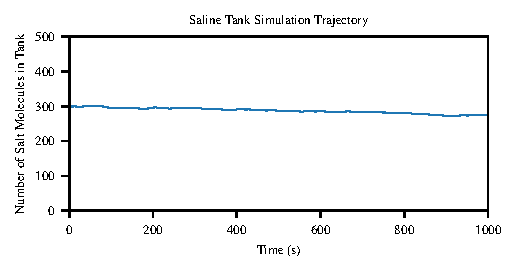
\includegraphics[width=\textwidth]{figures/saline_tank.pdf}
\caption{An example simulation from the model of Example~\ref{ex:saline_tank} with initial
condition $M(0) = 300 \textup{ NaCl molecules}$, parameters $V = 10^6\textup{ liters}$,
$a = b = 100\textup{ liters per hour}$,
$c=2.9112 \times 10^{-26}\textup{ grams per liter}$, assuming that one NaCl molecule has
mass $m = 9.704 \times 10^{-23}\textup{ grams}$, and with runtime $T=10^3\textup{ hours}$. We draw this with \PlotTrajs{} from \texttt{tools/plots/plot\_trajectories.py} (Listing~\ref{lst:plots_trajectories}).}
\label{fig:saline_tank}
\end{figure}

\end{example}


\begin{example}\label{ex:logistic_growth_code}
\textbf{Logistic Growth DG Simulation.}
Reconsider Example~\ref{ex:logistic_growth}, the logistic growth model. It is the simplest of our models: the state $P$ is a single population count changed by exactly two events. A birth increases $P$ by one and occurs at rate $rP$, and a death decreases $P$ by one and occurs at rate $rP^2/K$, where $r$ is the per-capita birth rate and $K$ is the carrying capacity. Table~\ref{tab:ode_events} lists the two events.

We simulate with a base doubling time $\tau = 36.5$ days, so that $r = \ln(2)/\tau$, a carrying capacity $K = 200$, an initial population $P(0) = 20$, and a run time $T = 365$ days.

In Figure~\ref{fig:bespoke_logistic_growth}, $\textsf{MakeRates}$ returns the birth rate $rP$ and the death rate $rP^2/K$ of Table~\ref{tab:ode_events}, and $\textsf{MakeDeltaStates}$ returns the state-change vector $(+1, -1)$, the $+1$ for a birth and the $-1$ for a death. Listing~\ref{lst:framework_logistic_growth} gives the \texttt{Python} implementation. It diverges from the pseudocode in deriving the per-capita rate $r = \ln(2)/\tau$ from the base doubling time, rather than taking $r$ directly.

\begin{figure}[htbp]
\centering
{\footnotesize
\adjustbox{valign=t}{\fbox{\procedure{$\textsf{MakeRates}(P,\, \theta) \to \vec{\lambda}$:}{
\pcind \pcreturn \left(rP,\; rP^2/K\right)
}}}\qquad
\adjustbox{valign=t}{\fbox{\procedure{$\textsf{MakeDeltaStates}(\theta) \to (\delta_j)_{j=1}^{N}$:}{
\pcind \pcreturn (+1,\, -1)
}}}\par}
\caption{The two bespoke subroutines for the logistic growth model. $\textsf{MakeRates}$ returns the birth and death rates, and $\textsf{MakeDeltaStates}$ returns the $\pm 1$ state changes, both following Table~\ref{tab:ode_events}. Compare to the \texttt{Python} in Listing~\ref{lst:framework_logistic_growth}.}
\label{fig:bespoke_logistic_growth}
\end{figure}

\lstinputlisting[float=htbp, language=Python, numbers=none, linerange={29-37}, caption={The bespoke \texttt{Python} functions for the logistic growth model, \MakeLogisticRates{} and \MakeLogisticDeltaStates{}. We pair these with the pseudocode of Figure~\ref{fig:bespoke_logistic_growth}.}, label={lst:framework_logistic_growth}]{../simulation_frameworks/logistic_growth.py}

The stochastic trajectories fluctuate around the deterministic logistic solution. Figure~\ref{fig:logistic_growth_mean_vs_ode} compares the mean of $30$ stochastic trajectories against the solution of Equation~\ref{eqn:logistic_growth}.

\end{example}


\begin{example}\label{ex:allee_code}
\textbf{Allee Effect DG Simulation.}
Reconsider Example~\ref{ex:allee} and the emperor's goal to estimate the probability that a colony goes extinct. We simulate trajectories with run times $T=2000$ days each and compute the sample proportion of simulations that go extinct. We assume the species has a base birth rate\index{birth rate} $r = 0.0045\textup{ days}^{-1}$, a cooperation threshold $L = 50\textup{ individuals}$, and a carrying capacity\index{carrying capacity} $K = 200\textup{ individuals}$. All colonies begin with $P(0) = 50$ individuals.

This system with these parameters has three equilibria. $P = 0$ and $P = K$ are stable equilibria, and $P = L$ is an unstable equilibrium. Trajectories with $0 < P < L$ or $P > K$ drift downward statistically. Trajectories with $L < P < K$ drift upward statistically. Since simulations start with $P(0) = 50 = L$, the first event is equally likely to be a birth or a death. About half of all trajectories will initially decrease and drift toward extinction. We therefore expect about half of all trajectories to end in extinction. Extinction is a permanent condition. Table~\ref{tab:allee_events} lists the four events.

\begin{table}[htbp]
\centering
\caption{Allee effect Doob-Gillespie events.}\label{tab:allee_events}
\begin{tabular}{llll}
\hline
Event & Description & Rate & $\Delta$State \\
\hline
Old-age death & Individual dies of old age & $\lambda_0 P$ & $-1$ \\
Sexual birth & Birth from sexual reproduction & $\lambda_0 P^2/K$ & $+1$ \\
Cooperative birth & Birth from cooperation & $\lambda_0 P^2/L$ & $+1$ \\
Competitive death & Death from over-competition & $\lambda_0 P^3/(KL)$ & $-1$ \\
\hline
\end{tabular}
\end{table}

In Figure~\ref{fig:bespoke_allee}, $\textsf{MakeRates}$ returns the four rates of Table~\ref{tab:allee_events} as the vector $(rP,\, rP^2/K,\, rP^2/L,\, rP^3/(KL))$, and $\textsf{MakeDeltaStates}$ returns the state-change vector $(-1, +1, +1, -1)$. Listing~\ref{lst:framework_allee} gives the \texttt{Python} implementation.

\begin{figure}[htbp]
\centering
{\footnotesize
\adjustbox{valign=t}{\fbox{\procedure{$\textsf{MakeRates}(P,\, \theta) \to \vec{\lambda}$:}{
\pcind \pcreturn \left(rP,\; \frac{r P^2}{K},\; \frac{r P^2}{L},\; \frac{r P^3}{KL}\right)
}}}\qquad
\adjustbox{valign=t}{\fbox{\procedure{$\textsf{MakeDeltaStates}(\theta) \to (\delta_j)_{j=1}^{N}$:}{
\pcind \pcreturn (-1,\, +1,\, +1,\, -1)
}}}\par}
\caption{The two bespoke subroutines for the Allee effect model, following Table~\ref{tab:allee_events}. Here $r$ is the base per-capita birth rate. Compare to the \texttt{Python} in Listing~\ref{lst:framework_allee}.}
\label{fig:bespoke_allee}
\end{figure}

The function \FindTraj{} (in the Python repository) inputs simulation setup data and a success condition function and returns a successful trajectory with a count of all attempts including the successful one. After running the Allee effect script (in the Python repository) with a sample of $128$ simulations, we saw $71$ simulations go extinct, providing an estimated probability of extinction $\widehat{p} = 0.5546875$ (see Section~\ref{subsec:background} for the definition of sample proportion and hat notation).
Verify that the qualitative behavior matches your ODE analysis: trajectories starting below $P = L = 50$ should drift toward extinction, while those starting above $L$ should drift toward $K = 200$.

\lstinputlisting[float=htbp, language=Python, numbers=none, linerange={9-19}, caption={\texttt{Python} functions \MakeAlleeRates{} and \MakeAlleeDeltaStates{} for the Allee effect model. See pseudocode in Figure~\ref{fig:bespoke_allee}.}, label={lst:framework_allee}]{../simulation_frameworks/allee_effect.py}

\begin{figure}[htbp]
\centering
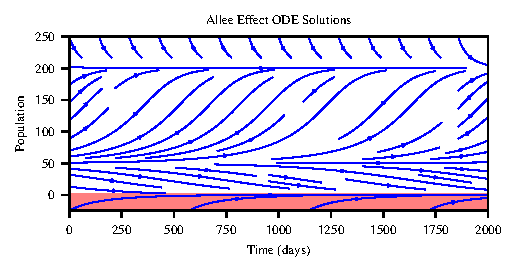
\includegraphics[width=\textwidth]{figures/allee_ode.pdf}
\caption{Phase diagram for Allee effect ODE $\frac{dP}{dt} = -rP(1-P/L)(1-P/K)$ ()$r = 0.0045\,\text{days}^{-1}$, $L = 50$, $K = 200$, from Example~\ref{ex:allee}).
Trajectories below $P = L$ trend to extinction. Trajectories above $P = L$ trend to $P = K$.
We shade the non-physical region $P < 0$ red. We draw this with \MakePhaseDiagram{} from \texttt{tools/plots/plot\_vector\_field.py} (Listing~\ref{lst:plots_vector_field}).}
\label{fig:allee_ode}
\end{figure}

\begin{figure}[htbp]
\centering
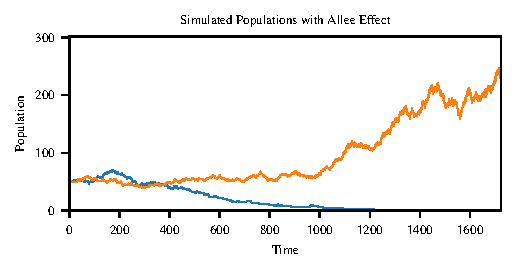
\includegraphics[width=\textwidth]{figures/allee_effect_two_trajs.pdf}
\caption{Two Allee trajectories from
Example~\ref{ex:allee}, with $r = 0.0045 (\text{time})^{-1}$,
$L = 50 \text{individuals}$, $K = 200$, and  $P(0) = 50$.  We draw this with \PlotTrajs{} from \texttt{tools/plots/plot\_trajectories.py} (Listing~\ref{lst:plots_trajectories}).}
\label{fig:allee_two_trajs}
\end{figure}


\begin{figure}[htbp]
\centering
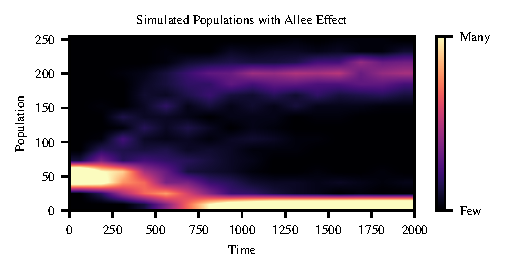
\includegraphics[width=\textwidth]{figures/allee_effect.pdf}
\caption{Heat map of $128$ Allee trajectories from Example~\ref{ex:allee} with the same parameters as Figure \ref{fig:allee_two_trajs}. Brighter pixels are near more trajectories.
We draw this with \PlotHeatmap{} from \texttt{tools/plots/plot\_heatmap\_histogram.py} (Listing~\ref{lst:plots_heatmap}).}
\label{fig:allee_heat}
\end{figure}

There are two types of stochastic trajectory. \textit{Successful} trajectories drift above $P(t) = L$ and reach the carrying capacity $P(t) = K$. \textit{Unsuccessful} trajectories slip below $P(t) = L$ and decline to extinction.
We use \PlotExtinctionAndSurvival{} to find two such trajectories in Figure~\ref{fig:allee_two_trajs}. See Section~\ref{subsec:plotting_utilities} for the plotting code.
The underlying ODE is scalar. We can therefore draw its phase diagram (Figure~\ref{fig:allee_ode}) as a streamplot in the $(t, P)$ plane. The streamlines confirm the three equilibria $P \in \{0, L, K\}$: trajectories starting below $L = 50$ converge to extinction, while those starting between $L$ and $K$ converge to the carrying capacity.
We generate a heat map of $128$ stochastic trajectories of the Allee model in Figure~\ref{fig:allee_heat}.
Nearly all trajectories fall into one of these two categories.
The heat map in Figure~\ref{fig:allee_heat} shows a proportion of simulations sweeping upward to the stable carrying capacity $P=K=200$, as well as a proportion falling below $P=L=50$ and ending near or at extinction.
The bright horizontal band around $P = 0$ at the end of the simulation indicates that many trajectories end in extinction.
The horizontal smear of brightness around $P = K = 200$ at the end of the simulation indicates that some trajectories survive at carrying capacity.
The darkness everywhere else indicate that trajectories don't spend a lot of time in the intermediate regions.
Hence, the distribution of simulation results at the end of the simulation is bimodal,\index{distribution!bimodal} with a cluster around $P = 0$ and a cluster around $P = K$.

As an aside, the state $P = 0$ is an absorbing state, so every window containing $P = 0$ contains many trajectories by the end of the simulation.
Thus, $P = 0$ appears very bright. In fact, in our Python code, we had to cap brightness to ensure that multimodal distributions would be visible.
The state $P = K$ is only probabilistically attracting, showing brightness in a haze around it, but trajectories wander nearby, dissipating their heat.
To make this graph, the heat map routine resamples every trajectory onto a common uniform time grid and then performs simple histogram binning.
That is to say, the heat indicates the residence of nearby trajectories, not the absolute number of nearby change-points.
See Section~\ref{subsec:plotting_utilities} for the heat-map plotting code and Section~\ref{subsubsec:prep_heatmap} for an explanation of this resampling.



The simulations are stochastic. Exceptions occur occasionally: trajectories bound for extinction that randomly wander above $P=L$ and recover to $P=K$, or trajectories near $P=K$ that randomly wander below $P=L$.

\end{example}


\begin{example}\label{ex:sir_code}
\textbf{SIR DG Simulation.}
Reconsider Example~\ref{ex:sir_first} and Charlie's fungus-infected cats. The SIR model partitions a population into three compartments: susceptible ($S$), infectious ($I$), and recovered ($R$). Individuals move from $S$ to $I$ upon infection and from $I$ to $R$ upon recovery. Assume Charlie has $S + I + R = 100$ cats, assume $I(0) = 10$ of the cats start out sick, and assume the rest are susceptible. We assume that cats recover with a half-life $\tau = 45$ days and interact with each other in random pairs $1000$ times a day, so the time between a cat's interactions is $\tau_{\textup{int}} = 1/1000 = 0.001$ days, and each interaction has a probability $0.0001$ (that is, $0.01\%$) of an infection spreading.
We use $\widetilde{\alpha} = \frac{0.0001}{0.001} = 0.1\,\textup{days}^{-1}$, and since $S + I + R = N = 100$, the per-pair rate is $\alpha = \widetilde{\alpha}/N = \frac{0.0001}{0.001 \cdot 100} = 10^{-3}\,(\textup{individual}\cdot\textup{days})^{-1}$, matching \MakeSirRates{} in the companion code.

We re-parameterize in terms of daily interactions because transmissibility depends on both the infectious organism and social behavior. For example, the black-tailed prairie dog is sociable, and plague (\textit{Yersinia pestis}) infections transmit rapidly through their populations. By contrast, California ground squirrels (\textit{Otospermophilus beecheyi}) are less social in their burrowing behavior and tolerate plague better than black-tailed prairie dogs \cite{buhnerkempe2011transmission}.

Unlike the previous models, the SIR state is a vector $(S, I, R)$ rather than a scalar count. Table~\ref{tab:sir_dg_events} lists the two events and their vector state changes.

\begin{table}[htbp]
\centering
\caption{SIR Doob-Gillespie events.}\label{tab:sir_dg_events}
\begin{tabular}{llll}
\hline
Event & Description & Rate & $\Delta$State \\
\hline
Infection & Susceptible becomes infectious & $\alpha S I$ & $(-1,+1,0)$ \\
Recovery & Infectious individual recovers & $\beta I$ & $(0,-1,+1)$ \\
\hline
\end{tabular}
\end{table}

In Figure~\ref{fig:bespoke_sir}, $\textsf{MakeRates}$ returns the infection rate $\alpha S I$ and the recovery rate $\beta I$ of Table~\ref{tab:sir_dg_events}, and, because the state is the vector $(S, I, R)$, $\textsf{MakeDeltaStates}$ returns the two vector changes $(-1, +1, 0)$ for an infection and $(0, -1, +1)$ for a recovery. Listing~\ref{lst:framework_sir} gives the \texttt{Python} implementation. It diverges from the pseudocode in two language- and model-specific ways: it derives $\alpha$ from the interaction time and infection probability and $\beta = \ln(2)/\tau$ from the recovery half-life, rather than taking $\alpha$ and $\beta$ directly, and it adds the chosen state change componentwise in \UpdateSirState{}.

\begin{figure}[htbp]
\centering
{\footnotesize
\adjustbox{valign=t}{\fbox{\procedure{$\textsf{MakeRates}((S,I,R),\, \theta) \to \vec{\lambda}$:}{
\pcind \pcreturn \left(\alpha S I,\; \beta I\right)
}}}\qquad
\adjustbox{valign=t}{\fbox{\procedure{$\textsf{MakeDeltaStates}(\theta) \to (\delta_j)_{j=1}^{N}$:}{
\pcind \pcreturn \left((-1, +1, 0),\; (0, -1, +1)\right)
}}}\par}
\caption{The two bespoke subroutines for the SIR model, following Table~\ref{tab:sir_dg_events}. Here $\alpha$ is the transmission rate and $\beta$ the recovery rate. The state change $\delta_j$ is a vector. Compare to the \texttt{Python} in Listing~\ref{lst:framework_sir}.}
\label{fig:bespoke_sir}
\end{figure}

\lstinputlisting[float=htbp, language=Python, numbers=none, linerange={13-29}, caption={The bespoke \texttt{Python} functions for the SIR model: \MakeSirRates{}, \MakeSirDeltaStates{}, and the componentwise update \UpdateSirState{}. We pair these with the pseudocode of Figure~\ref{fig:bespoke_sir}.}, label={lst:framework_sir}]{../simulation_frameworks/epidemiology.py}

We generate $100,000$ stochastic trajectories with run time $T = 365$ days (see the Python repository for the code) to estimate (i) the probability that Charlie's cats totally recover within a year and (ii) the five-number summary\index{summary, five-number} of the time until Charlie has no more infected cats, computed from trajectories in which all infectious cats recovered (i.e., $I = 0$) before day $365$. Our simulation reveals an estimated probability of total recovery within the year of $0.53844$ (a sample proportion, defined in Section~\ref{subsec:background}). The five-number summary (see Section~\ref{subsec:background}) of the time until recovery, computed only from trajectories in which all infectious cats recovered before day $365$, was $(161.5, 288.1, 315.9, 340.0, 364.998)$. This indicates that, when Charlie's cats totally recover within one year, a $50\%$ probability exists that the cats will take more than $316$ days to recover. We use the SIR plotting code (in the Python repository) to visualize one representative stochastic trajectory (which includes all three compartments of population members) in Figure~\ref{fig:sir}.

\begin{figure}[htbp]
\centering
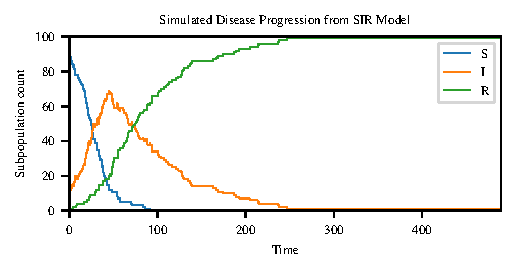
\includegraphics[width=\textwidth]{figures/epidemiology.pdf}
\caption{An example simulation of the fungal infection among Charlie's cats, showing the susceptible ($S$), infectious ($I$), and recovered ($R$) compartments over time. We draw this with \PlotTrajs{} from \texttt{tools/plots/plot\_trajectories.py} (Listing~\ref{lst:plots_trajectories}).}
\label{fig:sir}
\end{figure}

Verify that the qualitative behavior matches your ODE analysis: the susceptible compartment should fall monotonically, and the infectious compartment should peak and then decline as recovery outpaces new infections.

A streamplot like Figure~\ref{fig:ode_examples} does not apply here. A streamplot in the $(t, x)$ plane depicts the vector field $(1, f(t,x))$ for a scalar ODE $\dot{x} = f(t,x)$. The SIR state is the vector $(S, I, R)$ with conservation law $S + I + R = N$. The individual rates $\frac{dS}{dt} = -\alpha SI$ and $\frac{dI}{dt} = \alpha SI - \beta I$ each depend on two compartments. A phase portrait in the $(S, I)$ plane is possible, but it discards the time axis and does not give the timescale of the outbreak.

\end{example}




The examples above used sample proportions and five-number summaries to summarize simulation output. Section~\ref{subsec:background} introduces both. Section~\ref{subsec:output} formalizes their use, discusses when summary statistics can be misleading (particularly for bimodal output), and provides practical guidance for reporting stochastic simulation results. Read Section~\ref{subsec:output} before proceeding to sensitivity analysis (Section~\ref{subsec:qualitative_changes}), as the sensitivity analysis in Section~\ref{subsec:qualitative_changes} relies on the same statistical vocabulary.

\textup{{\bf Questions for Reflection:}}
\begin{enumerate}

\item Given $r, s > 0$ and the same initial condition $X_0 = Y_0$, the ODEs $\frac{dX}{dt} = rX$ and $\frac{dY}{dt} = (r+s)Y - sY$ always produce the same trajectories. Can you use the Doob-Gillespie algorithm to detect a difference between them? Explain.

\item In the deterministic Allee ODE, what happens as $L$ approaches $K$?

\item What can we expect from stochastic realizations of the Allee ODE as $L$ approaches $K$?

\item In the deterministic Allee ODE, what happens as we vary $r$?

\item What are some changes we can expect from the stochastic realizations of the Allee ODE as we vary $r$?

\item Consider the Allee-like model $\frac{dY}{dt} = rY(1-\frac{Y}{K})(1-\frac{Y}{L})(1-\frac{Y}{U})$ for some $K > L > U > 0$. Is this model suitable for describing a realistic ecological population with finite resources? Hint: Find the equilibria and determine whether birth or death is more likely near those equilibria.

\item How does your answer to the previous question change if we use $\frac{dY}{dt} = -rY(1-\frac{Y}{K})(1-\frac{Y}{L})(1-\frac{Y}{U})$ with the same $K > L > U > 0$? Hint: The sign change reverses time.

\item Interpret the notion of stochastic extinction with respect to the SIR model as presented in Example~\ref{ex:sir_first} as the occurrence that $S$ or $I$ randomly crashes to zero, and explain the impact on the remainder of the simulation when either of these compartments crashes to zero.

\item If an ODE has no oscillations near an equilibrium, the trajectories produced by the Doob-Gillespie algorithm are still stochastic and go up and down randomly, giving the illusion of oscillation. On the other hand, even if an ODE has oscillations near an equilibrium, the Doob-Gillespie trajectories are stochastic and may be strictly increasing or strictly decreasing for long intervals of time. Think about ways to detect whether a stochastic Doob-Gillespie implementation comes from an ODE that has oscillations.

\item After no susceptibles remain in the SIR model, $I$ changes like in the radioactive decay model with rate of decay $\beta$. Using $\beta = \ln(2)/45 \approx 0.0154\text{ days}^{-1}$, compute the ``half-life'' and interpret this half-life in terms of the original phenomena described by the SIR model. Check whether your computation of half-life makes sense by comparing it with Figure~\ref{fig:sir}.


\end{enumerate}

\section{Visualizing and Interpreting Simulated Trajectories}\label{sec:visualizing_interpreting}

%\textbf{Instructional Time:} 3 hours

\subsection{Visualizing Simulated Trajectories}\label{subsec:visualizing}

Section~\ref{sec:farming} produces trajectories. This subsection addresses how to display them. We plot stochastic trajectories rather than phase diagrams of deterministic ODE solutions. These trajectories hover near the deterministic solution but are noisy, discrete-state realizations, not smooth curves.

\subsubsection{A single trajectory is a step function}\label{subsubsec:single_traj_step}

Because the DG algorithm changes the state by exactly one integer at each event, the state remains constant between events and jumps discontinuously at each one. Thus, a stochastic trajectory the DG algorithm simulates is a piecewise-constant function\index{function!piecewise-constant} of time: the state holds constant between consecutive change points\index{change point} and jumps by $\pm 1$ at each event.

Consider a single run of the saline tank model (Example~\ref{ex:saline_tank_code}). The state variable is $M$, the number of NaCl molecules. The tank starts at $M = 300$ NaCl molecules. The deterministic equilibrium is $M \approx 150$, so the system is initially above equilibrium: departures are more likely than arrivals. After an exponentially distributed waiting time, the first event occurs. Suppose it is a departure. The state steps down to $M = 299$. We sample a new waiting time, the second event occurs, and the state steps again. The process repeats. Wait-times are random, so the events do not spread evenly in time. Sometimes, events occur often, with very little wait time. Sometimes, events occur seldomly, with long periods of stagnation. Over simulated time, many such steps accumulate. The result is a noisy staircase that drifts downward toward equilibrium and then fluctuates around it indefinitely.

This staircase is the raw output of the DG algorithm. Each changepoint $(t_i, M_i)$ is a corner of the step function, and the state is constant on each time interval $[t_i, t_{i+1})$. See Section~\ref{subsec:plotting_utilities} for the code that renders a stochastic trajectory as a step graph.

\subsubsection{Every run is different: motivating the heat map}\label{subsubsec:motivating_heatmap}

One trajectory is one sample from a distribution. Just as a single coin flip does not reveal the bias of the coin, a single trajectory does not reveal the probability of extinction or the range of typical outcomes.

Each run of the DG algorithm yields a distinct staircase. Two runs with the same initial conditions and parameters will agree in trend but differ in every individual step, because each waiting time and each event choice is random. Running the simulation $100{,}000$ times produces $100{,}000$ different staircases (usually).

If every run is different, how do we summarize all of them?

One approach is to overlay all trajectories on a single plot. For a small number of trajectories this works well, as seen in Figure~\ref{fig:allee_two_trajs}. For thousands of trajectories it produces an unreadable smear.

A more informative approach is a heat map:\index{heat map} a two-dimensional histogram over the $(t, Y)$-plane in which the color intensity of each cell is proportional to the number of simulated trajectories that pass through that cell. Cells that many trajectories visit appear bright. Cells that few visit appear dark. The heat map renders $100{,}000$ step functions as a single image. It shows whether the distribution of the state at a given time is unimodal,\index{distribution!unimodal} bimodal,\index{distribution!bimodal} or multimodal.

\subsubsection{Preparing trajectories for a heat map}\label{subsubsec:prep_heatmap}

Bright regions in a heat map show where many trajectories spend time. Multiple bright spots signal bimodal behavior.

The DG algorithm outputs change points at random times, not on a regular grid. To aggregate trajectories into a grid-based heat map, the heat map routine resamples every trajectory onto a common, uniform time grid before binning.
This piecewise-constant interpolation records the state at each grid time using the most recent changepoint, converting a sparse list of change points into a dense list of $(t, Y)$ pairs suitable for binning.

Filling at a random or too-coarse spacing introduces a small bias\index{heat map!binning bias} into the heat map.
When events occur frequently relative to the grid, several change points can fall between consecutive grid points, so the grid samples miss them and over-represent the states that happen to lie on grid lines. The bias worsens as events become more frequent. A finer partition reduces it, and we can show the error is $O(\Delta)$ in the grid spacing $\Delta$.
However, as $\Delta \to 0$, the graph approaches the unreadable smear we get when plotting all trajectories plainly, and there's a trade-off in cost. A heatmap with grid spacing $\Delta$ requires painting $O(\Delta^{-2})$ pixels. So in practice, we hand-tune $\Delta$ to get an informative heat map.

See Section~\ref{subsec:plotting_utilities} for the heat-map plotting code.

\subsection{The Plotting Utilities}\label{subsec:plotting_utilities}

We draw every figure in this chapter with one of four single-function modules in \texttt{tools/plots/}.
These modules are plotting code, not algorithms, so they have no pseudocode counterpart.
The scripts in \texttt{scripts/} use these tools to make the figures.
This way, the scripts play double duty as usage examples.

Three of our plotting utilities share one structure, the template of Listing~\ref{lst:plots_template}: set the page style, draw, then save or show.
Recall the template in Figure~\ref{fig:dg_algorithm} and Listing~\ref{lst:dg_algorithm_python_template} uses $\texttt{...}$ to mark the block in the DG algorithm which we must tailor for the ODE model.
Similarly, we use \texttt{...} to mark the block in the plotting template which we must tailor for the kind of image we generate.
The heat map follows the same template, but with an additional block that prepares the trajectories for binning before drawing.

Our plotting template's styling preamble converts two width fractions into \texttt{matplotlib} settings.
Publishers often resize images in LaTeX. The fraction \texttt{width\_frac} is the figure width as a fraction of the text width and \texttt{display\_frac} is the fraction at which we place the figure on the page, so their ratio \texttt{scale} undoes any later shrinkage.
The size \texttt{on\_page\_pt} is one point below the $10$-point body, which we rescale by \texttt{scale} to ensure that graph titles, legends, and labels have a common font size with the body. We store the width of the figure in inches in \texttt{width}.
Python's dictionary comprehension is sort of like set builder notation. We use it to store \texttt{on\_page\_pt} as font sizes for titles, labels, and legends in the dictionary \texttt{rc}. We use \texttt{rc.update} to add the serif font family, the STIX math font, $150$ dpi, the figure size, and a scaled line width. When a \texttt{latex} executable is on the path, the code enables \texttt{usetex} to match fonts. Writing \texttt{rc} into \texttt{rcParams} applies the settings.

After the drawing block, the tail sets the title and axis labels, tightens the margins, and either writes the figure to \texttt{save\_path}, creating its directory first, or shows it on screen.

\lstinputlisting[float=htbp, language=Python, numbers=none, caption={The shared template for the \texttt{tools/plots/} plotters. The styling preamble and the save-or-show tail are common to the trajectory, phase-diagram, and mean-versus-ODE plotters; each replaces the \texttt{...} block with its own drawing.}, label={lst:plots_template}]{../tools/plots/plot_template.py}

\subsubsection{Plotting trajectories}\label{subsubsec:code_plot_trajs}

The drawing block of \PlotTrajs{} (Listing~\ref{lst:plots_trajectories}) renders trajectories as step graphs. \texttt{draw\_labels} substitutes a list of \texttt{None} when the caller gives no labels, keeping the loop uniform. The loop unzips each trajectory into times and states and draws it as a right-continuous step (\texttt{where='post'}). A legend appears only when the caller supplies real labels. The \texttt{xlim} and \texttt{ylim} calls fix the axis ranges to the supplied bounds.

\lstinputlisting[float=htbp, language=Python, numbers=none, linerange={29-37}, caption={The drawing block of \PlotTrajs{} in \texttt{tools/plots/plot\_trajectories.py}, which we insert into the template of Listing~\ref{lst:plots_template}. It draws Figures~\ref{fig:saline_tank}, \ref{fig:allee_two_trajs}, and~\ref{fig:sir}.}, label={lst:plots_trajectories}]{../tools/plots/plot_trajectories.py}

\subsubsection{Plotting phase diagrams}\label{subsubsec:code_phase}

The drawing block of \MakePhaseDiagram{} (Listing~\ref{lst:plots_vector_field}) draws the streamplot of a scalar ODE. \texttt{mgrid} builds a grid of resolution \texttt{res} over the time-state rectangle. The horizontal arrow component is $1$ since time advances at unit rate, and the vertical component is the caller's \texttt{y\_len\_fun} on the grid. To use this to make a phase diagram of an ODE of the form $y^\prime = f(y)$, just express $f(y)$ as \texttt{y\_len\_fun}. The \texttt{streamplot} call draws the field in blue with arrow size scaled to the page, and an optional \texttt{axhspan} shades the non-physical region below zero red.

\lstinputlisting[float=htbp, language=Python, numbers=none, linerange={31-38}, caption={The drawing block of \MakePhaseDiagram{} in \texttt{tools/plots/plot\_vector\_field.py}, which we insert into the template of Listing~\ref{lst:plots_template}. It draws the phase diagrams in Figures~\ref{fig:ode_examples} and~\ref{fig:allee_ode}.}, label={lst:plots_vector_field}]{../tools/plots/plot_vector_field.py}

\subsubsection{Plotting the mean against the ODE}\label{subsubsec:code_mean}

The drawing block of \PlotMeanVsOde{} (Listing~\ref{lst:plots_mean_vs_ode}) overlays a stochastic mean on a deterministic solution. An optional \texttt{axhspan} shades the non-physical region. The code plots the stochastic mean as a solid curve and the ODE solution as a dashed curve, sets the axes to the data range, and places a legend at the lower right.

\lstinputlisting[float=htbp, language=Python, numbers=none, linerange={29-35}, caption={The drawing block of \PlotMeanVsOde{} in \texttt{tools/plots/plot\_mean\_vs\_ode.py}, which we insert into the template of Listing~\ref{lst:plots_template}. It draws Figure~\ref{fig:logistic_growth_mean_vs_ode}.}, label={lst:plots_mean_vs_ode}]{../tools/plots/plot_mean_vs_ode.py}

\subsubsection{Plotting the heat map}\label{subsubsec:code_heatmap}

The heat map follows the template, adding a block that prepares the trajectories before the drawing block.
\PlotHeatmap{} (Listing~\ref{lst:plots_heatmap}) first re-samples trajectories by laying \texttt{grid} equal time bins, finding their centers, and reading each trajectory's state at those centers by looking at the latest change point with \texttt{searchsorted}. Section~\ref{subsubsec:prep_heatmap} explains why this matters. \PlotHeatmap{} then stacks the re-sampled trajectories. \texttt{histogram2d} bins the $(t, y)$ pairs into a \texttt{grid}-by-\texttt{grid} count array. This count array determines brightness, but we cap the brightness at the $95$th percentile of counts as \texttt{vmax}. This way, the brightest cells saturate while dimmer occupancy bands stay visible, showing multimodal distributions. Finally, the code draws the transposed counts as a rasterized image with the \texttt{magma} colormap and bilinear smoothing, adds a color bar labeled from \emph{Few} to \emph{Many}, labels the axes, and saves or shows the figure through the shared tail.

\lstinputlisting[float=htbp, language=Python, numbers=none, linerange={30-55}, caption={The drawing block of \PlotHeatmap{} in \texttt{tools/plots/plot\_heatmap\_histogram.py}, which we insert into the template of Listing~\ref{lst:plots_template}. It draws the heat map in Figure~\ref{fig:allee_heat}.}, label={lst:plots_heatmap}]{../tools/plots/plot_heatmap_histogram.py}

\subsection{Reading and Statistically Measuring Stochastic Output}\label{subsec:output}

%\textbf{Instructional Time:} 1 hour

Examples~\ref{ex:saline_tank_code}, \ref{ex:allee_code}, and \ref{ex:sir_code} reported results as sample proportions and five-number summaries without justifying why these statistics are appropriate or how to interpret them. We provide a light refresher on statistics in this section.

\subsubsection{Sample proportion as a probability estimator}\label{subsubsec:sample_proportion}

As a rule, if the event has probability $p$, run at least $1/p$ simulations to observe it reliably. For rare events ($p$ near $0$), you need much larger samples.

Many questions about a model reduce to a binary outcome: does the population go extinct? Does the process succeed before time $T$? Does the state ever exceed a threshold? For any such binary event with true probability $p$, a large sample of $n$ independent simulations, and $k$ observations, the sample proportion\index{proportion, sample} $\hat{p} = k/n$ is an unbiased estimator\index{estimator, unbiased} of $p$: on average, $\hat{p} = p$. The precision of $\hat{p}$ improves as $n$ increases, with standard error $\sqrt{p(1-p)/n}$.

If $\hat{p} = 3/100{,}000 = 3\times 10^{-5}$, the estimate is not robust: observing even one less observation would reduce our estimate to $2/100{,}000$, a $50\%$ drop.

\subsubsection{Five-number summary for a continuous-valued statistic}\label{subsubsec:five_number}

The mean is misleading for skewed or multimodal distributions. The five-number summary\index{summary, five-number} describes center, spread, and extremes without assuming a symmetric shape.

When the statistic of interest is continuously valued (for example, the time until extinction, the time until full recovery, or the peak state), the five-number summary (see Section~\ref{subsec:background}) provides a concise description of the distribution without assuming any parametric form.

In Example~\ref{ex:sir_code}, we restricted to the simulations in which all cats recovered within the year.
We computed the five-number summary of the recovery time and saw the following.
\begin{itemize}
\item The fastest recovery took about $161.5$ days ($Q_0 = \min$).
\item The median recovery time was about $316$ days.
\item $75\%$ of recoveries took more than $288$ days ($Q_1$).
\item The slowest recovery in the sample reached $364.998$ days ($Q_4 = \max$), strictly inside the simulation window.
\end{itemize}
Determining these statistics requires no distributional assumption (normal, exponential, etc.). We call the five-number summary \textit{non-parametric}.

\subsubsection{Non-unimodal distributions and their interpretation}\label{subsubsec:non_unimodal}

Before coming to any conclusions, inspect whether the distribution is unimodal. Conclusions based on the mean or median for a strongly bimodal or multimodal distribution is misleading, because the central value may fall in a trough between two peaks where few trajectories reside.

The Allee effect simulation (Example~\ref{ex:allee_code}) illustrates this. The heat map in Figure~\ref{fig:allee_heat} shows two distinct clusters of trajectories at the end of the simulation: one near the stable carrying capacity $K = 200$ and one near extinction\index{extinction!stochastic} at $P = 0$. The distribution of final states is strongly bimodal. A single average final state conveys almost no useful information.

The conditional distribution of the final state given survival, i.e.\ the \textit{survivorship bias}, is more informative, but is misleading for its own reasons. Statistical patterns which matter only indirectly are less informative than direct causes, and those are less informative than firm predictions. Like a good prediction of weather should provid a probability of rain, a good analysis of a population ecology model should estimate extinction probability $\hat{p}$.

No matter the stastics we decide to measure, it is wise to inspect a heat map or histogram of the simulation output. If the distribution has more than one mode, partition the trajectories into qualitatively distinct groups and perform separate statistical analyses for each group.

\textup{{\bf Questions for Reflection:}}
\begin{enumerate}
\item A social researcher finds that the average American family has decreased in size from $1.7$ parents and $2.3$ children to $1.1$ parents and $1.9$ children. Explain why this might be misleading and discuss what you would report instead.

\item The heat map of the Allee effect simulation shows two bright bands at $P = 0$ and $P = K$ at time $T$; extinction appears highly likely, say with probability $p$. Using the standard-error rule from Section~\ref{subsec:output}, approximately how many simulations do you need to estimate $p$ with a standard error of at most $0.01$?

\item The heat map routine records the state at each grid time using the last observed state before that time. A colleague suggests linear interpolation between change points instead. Describe one scenario in which linear interpolation would give a visually smoother heat map yet misrepresent the true probability distribution of the process.
\end{enumerate}



\section{Parameter Space Exploration}\label{sec:parameter_sweep}\index{exploration!parameter space}\index{parameter space exploration}

%\textbf{Instructional Time:} 3 hours

A parameter sweep surveys how a model behaves across a range of parameter values. Such sweeps are costly, but they show how sensitive the model is to measurement error in its parameters and reveal qualitative changes in behavior that a single run hides.

The sweep steps through part of the parameter space, generates many stochastic trajectories for each parameter combination, and collects summary statistics. We perform a small-scale sweep for the logistic growth model\index{logistic growth} in Example~\ref{ex:exploration}. The same approach applies to any of the models in this chapter.

Readers who recreate the results below will see different numbers, even with the same parameters and sample sizes, because the DG algorithm is stochastic.


\subsection{Exploring Parameter Space}\label{subsec:exploring_parameter_space}

%\textbf{Instructional Time:} 2 hours

We select two parameters $r$ and $K$ from small sets of possibilities and measure two statistics across those choices.

\begin{example}\label{ex:exploration}
\textbf{Logistic Growth Parameter Space Exploration.}
We revisit Example~\ref{ex:logistic_growth}. Assuming all simulations start with their populations at half their carrying capacity\index{carrying capacity}, we explore the parameter space by determining two statistics: the proportion\index{proportion, sample} of simulations out of $100$ that go extinct within $365$ days, $p_{\texttt{extinct}}$ and the proportion of simulations in which the population exceeds its carrying capacity within $365$ days, $p_{\texttt{cap}}$.

These are not mutually exclusive events, and neither may occur during a simulation. We investigate simulations with $r = \ln(2)/\tau$, where $\tau$ is a base population doubling time varying uniformly between some minimal and maximal value. We select $\frac{1}{8}$ of the total simulation time as the minimal value of $\tau$ and $\frac{1}{2}$ as the maximal value of $\tau$. The total simulation time is $365$ days and $\tau$ is measured in days, so the smallest growth rate is $r = \ln(2)/(365/2) \approx 0.0038\,\text{day}^{-1}$ and the largest is $r = \ln(2)/(365/8) \approx 0.0152\,\text{day}^{-1}$. We use $r \in \left\{0.0038, 0.0047, 0.0061, 0.0087, 0.0152\right\}\,\text{day}^{-1}$ and we explore carrying capacities $K \in \left\{10, 32.5, 55, 77.5, 100\right\}$.

Higher precision in both $r$ and $K$ is possible, but the stochasticity of the DG algorithm washes it out except when large samples are feasible. This is a property of the exponential distribution from which we sample durations between events. Four decimals of precision in $r$ suffice for up to $10,000$ simulations, provided each simulation lasts $365$ days.

See Table~\ref{table:pcap} for the resulting $p_{\texttt{cap}}$ estimates. Logistic populations starting at $K/2$ effectively never go extinct over $365$ days, so $p_{\texttt{extinct}}$ is negligible across this grid and we tabulate only $p_{\texttt{cap}}$. The code for \MakeLogisticRates{} and \DgSimulateLogisticOde{} is in the Python repository (\url{https://github.com/b-g-goodell/stoch-ode}). The constants ${\tt LOGISTIC\_SAMPLE\_SIZE} = 100$ and ${\tt PARAMETER\_SPACE\_EXPLORATION\_RESOLUTION} = 5j$ configure the number of trajectories per parameter combination and the resolution of the parameter grid, here a $5 \times 5$ grid matching Table~\ref{table:pcap}. The suffix $j$ is Python's notation for $\sqrt{-1}$. Passing it to \texttt{mgrid} signals that the preceding integer is a point count rather than a step size.

The logistic growth DG simulation models two competing events at each step, listed with their rates in Table~\ref{tab:ode_events}.


\begin{table}[htbp]
\centering
\begin{tabular}{||c | c | c | c | c | c ||}
 \hline
 $p_{\textup{cap}}$ & $K = 10$ & $K = 32.5$ & $ K = 55$ & $ K = 77.5$ & $K = 100$ \\ [0.5ex]
 \hline\hline
 $r = 0.0038$ & $0.309$ & $0.181$ & $0.093$ & $0.05$ & $0.026$ \\
 \hline
 $r = 0.0047$ & $0.388$ & $0.26$ & $0.207$ & $0.155$ & $0.107$  \\
 \hline
 $r = 0.0061$ & $0.528$  & $0.485$ & $0.369$ & $0.332$ & $0.255$ \\
 \hline
 $r = 0.0087$ & $0.66$  & $0.71$ & $0.659$ & $0.601$ & $0.61$ \\
 \hline
 $r = 0.0152$ & $0.862$  & $0.942$ & $0.936$ & $0.934$ & $0.937$ \\
 \hline
\end{tabular}
\caption{Estimates of $p_{\textup{cap}}$, the proportion of logistic-growth simulations (out of $100$) whose population exceeds the carrying capacity within $365$ days, across growth rates $r$ (rows) and carrying capacities $K$ (columns).}
\label{table:pcap}
\end{table}


\end{example}


\subsection{Scale and Cost of Parameter Space Exploration}\label{subsec:scale_cost_parameter_sweep}

%\textbf{Instructional Time:} 1 hour

A thorough parameter space exploration spans more than one order of magnitude for each parameter, with more than one sample point per order of magnitude. For example, using $r \in \left\{10^{-3}, 10^{-2.9}, 10^{-2.8}, \ldots, 10^{2.8}, 10^{2.9}, 10^3\right\}$ (there are $61$ possible choices of $r$ in this set) and $K \in \left\{10^1, 10^{1.1}, 10^{1.2}, \ldots, 10^{5.8}, 10^{5.9}, 10^6\right\}$ (there are $51$ choices of $K$ in this set) would be more appropriate. This would require generating a sample size $N$ of simulations for each of these $51\cdot 61 = 3111$ different parameter choices.

Parameter space exploration is computationally costly. It also suffers the \textit{curse of dimensionality}\index{curse of dimensionality}, a phrase describing the explosive growth in the number of cases to check as the number of parameters grows. With 5 parameters each taking 10 values, a complete sweep requires 100,000 simulation runs. Adding one more parameter multiplies the work tenfold. Given $m$ parameters with $n$ possible values, there are $n^m$ total parameter choices. Checking ``only'' $n=30$ possibilities for $m=50$ different parameters requires generating $30^{50} N$ simulation results. The number $30^{50}$ is astronomically large, far more simulations than anyone could ever run.

This trade-off deepens because parameter space exploration is most useful when the researcher can individually inspect plots of simulated results to identify qualitatively different behaviors.
In a weird version of Heisenberg's uncertainty principle, the more thoroughly we search the parameter space, the less thoroughly we can inspect simulation results.
Estimate the total runtime of a parameter sweep before launching it.

\textup{{\bf Questions for Reflection:}}
\begin{enumerate}
\item In Table~\ref{table:pcap}, $p_{\text{cap}}$ is uniformly high across all values of $K$ when $r = 0.0152$, but depends strongly on $K$ when $r = 0.0038$. Using the logistic growth event rates, explain analytically why a higher growth rate makes exceeding the carrying capacity likely regardless of $K$.

\item You have $m = 6$ parameters and a computational budget of $10^6$ simulation runs, each lasting one simulated year. A complete factorial design with $n$ values per parameter requires $n^6$ runs. How many values per parameter does the budget allow? Propose an alternative sampling strategy that uses the budget more efficiently without sacrificing coverage of qualitatively distinct regions.

\item Parameter space exploration is most useful when a researcher visually inspects each result, but inspection does not scale to thousands of plots. Using only the statistical tools introduced in this chapter, propose an automated summary for parameter sweep output and identify what information it loses compared to visual inspection of individual plots.
\end{enumerate}


\section{Model Sensitivity Analysis}\label{sec:sensitivity_analysis}\index{analysis!sensitivity}\index{sensitivity analysis}

%\textbf{Instructional Time:} 4 hours

Sensitivity analysis quantifies how model outputs respond to changes in individual parameters. It tells us whether simulation results are reliable given the precision of our parameter measurements. It belongs to the analysis and model assessment stage of the modeling cycle: once we have a solution, we judge how much to trust it.

If the model is highly sensitive to a parameter $r$, small errors in measuring $r$ can produce qualitatively different simulation outputs. The researcher must then secure high-precision, high-accuracy estimates of $r$. If the model is insensitive to $r$, even rough estimates suffice.

The elasticity score we define below uses sample statistics (sample proportions\index{proportion, sample}, five-number summaries\index{summary, five-number}) introduced in Section~\ref{subsec:background} and used throughout Section~\ref{sec:farming}. Readers should consult Section~\ref{subsec:output} on reading stochastic output before proceeding. An elasticity score derived from a bimodal output distribution can be severely misleading.

We use a scalar elasticity score, the univariate elasticity, and apply it to the logistic growth model\index{logistic growth} from Example~\ref{ex:logistic_growth}. Bifurcations\index{bifurcation}, qualitative changes in model behavior, can make the score misleading, so we address them as well. The same methods apply to any model in this chapter.


\needspace{5\baselineskip}
\subsection{Assessing and Interpreting Univariate Model Sensitivity}\label{subsec:elasticity}\index{elasticity!univariate}

%\textbf{Instructional Time:} 2 hours

To stochastically simulate trajectories of an ODE model, we must parameterize it from empirical observations, which always have error margins. Model sensitivity measures how much those error margins affect the simulation output.

One definition of model sensitivity is \textit{univariate elasticity}\index{elasticity!univariate} of an observed statistic $V(r)$. The word `elasticity' comes from economics, where it measures how sensitive demand is to a price change. Here it plays the same role: if we change one parameter $r$ by a small percentage, by what percentage does our simulation output $V$ change?

Elasticity answers the question ``if I mismeasure a parameter by 10 percent, how wrong will my output be?''

\begin{definition}[Elasticity of $V$]\label{def:elasticity}
Let $r, s > 0$ with $r \neq s$, and let $V(r), V(s) > 0$. The \textit{elasticity of $V$ at $(r,s)$}, written $\mathcal{E}_{V}(r,s)$, is
\[\mathcal{E}_{V}(r,s) = \frac{\ln V(r) - \ln V(s)}{\ln r - \ln s}.\]
Elasticity is unitless: $\ln(V(r)/V(s))$ and $\ln(r/s)$ are dimensionless ratios.
\end{definition}

The definition requires $V(r), V(s) > 0$, since the logarithm of a non-positive statistic is undefined. A parameter sweep can produce a statistic equal to $0$ or $1$ (for instance, an extinction proportion of $0$). In that case, apply a continuity correction, or for a probability replace it with its odds $V/(1-V)$, before computing elasticity.

For example, say $r, s$ are birth rates in the logistic growth model such that $r \approx 1.1 \cdot s$, say $V$ is the average time until extinction in a stochastic simulation, and presume $V(r) \approx 1.05 \cdot V(s)$. Then $r/s = 1.1$, $V(r)/V(s) = 1.05$, so $\mathcal{E}_{V}(r,s) = \frac{\ln(1.05)}{\ln(1.10)} \approx 0.512$. The sign is positive: when $r > s$, we see $V(r) > V(s)$. The value near $\frac{1}{2}$ says the relative change in $V$ is about half the relative change in $r$.

Now, maintain the assumption that $r \approx 1.1 \cdot s$, but presume $V(r) \approx 0.8 \cdot V(s)$ instead. Then $\mathcal{E}_{V}(r,s) = \frac{\ln(0.8)}{\ln(1.10)} \approx -2.341$. The sign is negative: when $r > s$, we see $V(r) < V(s)$. The value $-2.341$ says the relative change in $V$ is about two to three times the relative change in $r$ in magnitude.

The magnitude of $\mathcal{E}_{V}(r,s)$ sorts sensitivity into three regimes.
\begin{itemize}
\item $\left|\mathcal{E}_{V}(r,s)\right| \approx 1$: $V$ is approximately linearly sensitive to $r$. One order-of-magnitude change in $r$ leads to about one order-of-magnitude change in $V(r)$.
\item $\left|\mathcal{E}_{V}(r,s)\right| < 1$: $V$ is sub-linearly sensitive to $r$. $V(r)$ suppresses error margins on $r$, so even rough parameter estimates may suffice.
\item $\left|\mathcal{E}_{V}(r,s)\right| > 1$: $V$ is super-linearly sensitive to $r$. $V(r)$ amplifies error margins on $r$, requiring high-precision parameterization.
\end{itemize}

If $r \neq s$ are both positive, then $r = \mu s$ for some $\mu > 0$. When $\mu$ is close to $1$, $r$ is close to $s$, corresponding to small error margins. Using the definition of $\mathcal{E}$, the relationship between $V(r)$ and $V(s)$ is:
\begin{align*}
\mu^{\mathcal{E}} = \frac{V(r)}{V(s)}, \qquad \text{i.e.,} \qquad V(r) = \mu^{\mathcal{E}} V(s).
\end{align*}
Inspecting this equation, note the following qualitative trends.
\begin{itemize}
\item If $\mathcal{E} \gg 0$ and $\mu > 1$, then $V(r) > V(s)$.
\item If $\mathcal{E} > 0$ and $\mu \approx 1$, then $V(r) \approx V(s)$.
\item If $\mathcal{E} \gg 0$ and $\mu < 1$, then $V(r) < V(s)$.
\end{itemize}
Using similar reasoning, try to work out trends corresponding to the scenarios where $\mathcal{E} \approx 0$ and $\mathcal{E} \ll 0$. Note why $\mu$ and $\mathcal{E}$ must be unitless: $\mu^{\mathcal{E}}$ is a multiplicative factor.

\begin{example}\label{ex:basic_sensitivity_analysis}
\textbf{Sensitivity of Logistic Growth to $r$ and $K$.}
From Example~\ref{ex:exploration}, we can select any two entries in the same column or row in Table~\ref{table:pcap} and estimate the elasticity using those values.

For example, if $r = 0.0047$, then as we vary $K$ from $K_1 = 10$ to $K_2 = 100$, we have \[\mathcal{E}_{V}(K_1,K_2) = \frac{\ln(0.388) - \ln(0.107)}{\ln(10) - \ln(100)} \approx -0.559.\]
The negative sign indicates that the ``slope'' of $p_{\text{cap}}$ with respect to $K$ is negative.
That is to say, if $K$ increases, then $p_{\text{cap}}$ decreases. This makes intuitive sense, because if $K$ large compared to the population's current effective per-capita birth rate, it will take a simulation a longer time than $365$ days to attain the carrying capacity.
records the inverse relationship between the probability of exceeding carrying capacity and $K$. Since $\left|\mathcal{E}_{V}(K_1,K_2)\right| < 1$, the model is insensitive as we vary $K$, and because the magnitude is near $1/2$, approximately quadrupling carrying capacity is necessary to halve the probability of exceeding carrying capacity. The model is therefore forgiving of inaccurate or imprecise measurements of $K$.

On the other hand, if $K = 32.5$, then varying $r$ from $r_1 = 0.0038$ to $r_2 = 0.0152$ gives
\[\mathcal{E}_{V}(r_1,r_2) = \frac{\ln(0.181) - \ln(0.942)}{\ln(0.0038) - \ln(0.0152)} \approx 1.190.\]
Since $\mathcal{E}_{V}(r_1,r_2) > 1$ and positive, this indicates model sensitivity as we vary $r$, with a direct relationship between the probability of exceeding carrying capacity and $r$. The model is moderately sensitive to $r$.
\end{example}


\begin{example}[Parameterizing the Logistic Growth Model]\label{ex:logistic_growth_parameterizing}
Suppose a field study reports that a population of California ground squirrels breeds approximately once per year (birth interval $T_b \approx 1$ year), with adult lifespan $T_\ell \approx 4$ years, and typical colony size $K \approx 180$ individuals. We set
\[r = \frac{1}{T_b} - \frac{1}{T_\ell} = 1 - 0.25 = 0.75 \text{ year}^{-1}, \qquad K = 180.\]
These are rough estimates derived from life-history data. The roughness warrants sensitivity analysis to assess how much the simulation output changes if, say, $r$ is off by 20\%. Computing $\mathcal{E}_{V}(r, s)$ with $s = 0.8 \cdot r = 0.6$ or $s = 1.2 \cdot r = 0.9$ gives a practical measure of how consequential that measurement error is.
\end{example}

\textup{{\bf Questions for Reflection:}}
\begin{enumerate}
\item In Example~\ref{ex:basic_sensitivity_analysis}, we showed $\mathcal{E}_{V}(K_1,K_2) \approx -0.56$ when $r = 0.0047$ and $K$ is in the interval $[10, 100]$. What happens outside this range? Why?
\item Consider the sensitivity of the SIR model, when measuring the \textit{odds of extinction} as $V$. If $p$ is the probability of extinction, then the odds of extinction is the statistic $\frac{p}{1-p}$. What happens if we cannot estimate odds of extinction because every simulation stochastically resulted in the first infected individual recovering? What can we do to handle the situation?

\item The elasticity formula $\mathcal{E}_V(r,s)$ uses two concrete parameter values rather than an infinitesimal perturbation. Explain why choosing $r$ and $s$ very close together can be unreliable in practice when simulation estimates $V$, and how a practitioner should choose the gap between them.
\end{enumerate}

\subsection{Controlling for Qualitative Changes in Behavior}\label{subsec:qualitative_changes}

%\textbf{Instructional Time:} 2 hours

A bifurcation is a parameter value at which the qualitative behavior of the model changes abruptly. A population under a constant harvest\index{model!harvest} may settle to a stable size when the harvest rate is low, but may crash to extinction\index{extinction!stochastic} if the harvest rate exceeds a certain threshold.
The parameter value at which this transition occurs is the \textit{bifurcation point}\index{bifurcation!point}.

Bifurcations merit independent study. Kuznetsov \cite{kuznetsov1998elements} provides a rigorous treatment of bifurcation theory for ODE systems.
When a parameter change shifts the model into a different behavioral regime, the analysis must account for that shift.
Bifurcations are worth identifying because the elasticity formula $\mathcal{E}_{V}(r,s)$ can give misleading results when $r$ and $s$ straddle a bifurcation point. We call a complete analysis of all bifurcation points in a system a \textit{bifurcation portrait}\index{bifurcation!portrait}.

Formally constructing a bifurcation portrait is involved. Elasticity is a useful back-of-the-envelope diagnostic for determining whether a bifurcation has occurred. A sharp change in elasticity is a sign to partition the parameter space, so that the results we compare within one region share the same qualitative behavior.

\begin{example}\label{ex:const_harvest}
\textbf{Logistic Growth under Constant Harvest.}
Here is an ecological model of an organism with a population capacity under constant harvest. Let $r, K, \alpha > 0$.
\begin{align*}
\frac{dP}{dt} &= rP(1-\frac{P}{K}) - \alpha
\end{align*}
Observe the following about this model.
\begin{enumerate}[(i)]
\item The units of $\frac{dP}{dt}$ are in individuals per unit time (say $I/t$). So the units of the right hand side are also individuals per unit time, $I/t$. This provides the units of $\alpha$ as the $I/t$, number of individuals harvested per unit time. Note that if $K$ is in units of individuals, then $1 - \frac{P}{K}$ is unit-less. Hence, $r$ has units $1/t$.

\item We have a steady-state solution when $\frac{dP}{dt} = 0$. Solving gives $-\frac{r}{K}P^2 + rP - \alpha = 0$. The quadratic formula gives us steady-state solutions when $P = P^* = \frac{K}{2}\left(1 \pm \sqrt{1-\frac{4\alpha}{rK}}\right)$. Since $P(t)$ is a non-negative number, a negative or complex steady state indicates an unrealistic trajectory that does not correspond with a real-life scenario.

\item If $\alpha > 0$, the origin $P=0$ is not an equilibrium, and a trajectory starting here has $\frac{dP}{dt} = -\alpha < 0$. When $\alpha < \frac{rK}{4}$, write the two steady states as $P_- = \frac{K}{2}\left(1 - \sqrt{1-\frac{4\alpha}{rK}}\right)$ and $P_+ = \frac{K}{2}\left(1 + \sqrt{1-\frac{4\alpha}{rK}}\right)$, with $P_- < P_+$. A trajectory with $P_0 < P_-$ has $\frac{dP}{dt} < 0$, so it is strictly decreasing and falls to extinction (becoming negative and unbounded below if we do not stop the simulation). A trajectory with $P_- < P_0 < P_+$ instead rises to the stable upper equilibrium $P_+$. To prevent numerical overflow errors during simulations, we terminate the simulation when $P=0$.

\item Note that if $\alpha < \frac{rK}{4}$, then there exist two real steady state solutions. If $\alpha = \frac{rK}{4}$, then there is exactly one real steady state solution. If $\alpha > \frac{rK}{4}$, then there are no real steady state solutions. This suggests a qualitative difference in the behavior of the system when $\alpha < \frac{rK}{4}$, when $\alpha = \frac{rK}{4}$, and when $\alpha > \frac{rK}{4}$. In fact, these are three distinct dynamical regimes, one for each case below.

\begin{itemize}
\item When $\alpha < \frac{rK}{4}$, there are two steady state solutions. The greater of the two is a stable equilibrium, and the lesser of the two is an unstable equilibrium. The farther away from $\frac{rK}{4}$ we can make $\alpha$, the lower the likelihood of stochastic extinction and the longer the residence time near the stable steady state solution. As $\alpha$ approaches $\frac{rK}{4}$, the two steady state solutions get close to each other. The \textit{basin of attraction}\index{attraction, basin of}\index{basin of attraction} around the stable steady state is the set of initial conditions from which the population will eventually approach the steady state. The basin of attraction gets smaller as these two solutions approach each other. The amount of time trajectories spend near the stable steady state solution decreases, and trajectories wander further and wider. Consequently, stochastic extinction becomes more likely.
\item When $\alpha = \frac{rK}{4}$, one steady state solution exists, and we call it ``half-stable:''\index{equilibrium!half-stable} trajectories coming from above tend to linger, and trajectories from below tend to escape. In practice this means that any small random downward fluctuation pushes the population irreversibly toward extinction. The ``half-stable'' point is a temporary stop on the way to extinction, because death events are more likely than birth events on both sides of the equilibrium. The likelihood of stochastic extinction is greater than when $\alpha < \frac{rK}{4}$, and residence time at the steady state solution is as low as can be.
\item When $\alpha > \frac{rK}{4}$, no steady state solution exists, and the likelihood of stochastic extinction approaches certainty. There is no residency time near the steady state solution, because there is no steady state solution.
\end{itemize}

\end{enumerate}

We have three classes of parameters: $\alpha < \frac{rK}{4}$, $\alpha = \frac{rK}{4}$, and $\alpha > \frac{rK}{4}$. Moreover, we expect qualitatively similar trajectories from the case $\alpha = \frac{rK}{4}$ and the case $\alpha > \frac{rK}{4}$ due to the aforementioned ``half-stable'' point. Thus, these conditions define three different parametric cases to study, and we have reason to believe that two of them lead to dynamic regimes which are qualitatively similar (a convenient hypothesis to test with simulations).

\end{example}

$\mathcal{E}_{V}(r,s)$ is a finite-difference approximation of a kind of logarithmic derivative, meaningful only when the function it approximates is smooth, with no sudden jumps or tears. In Example~\ref{ex:const_harvest}, the statistic $V$ behaves differently depending on which side of the bifurcation point $\frac{rK}{4}$ the harvest rate $\alpha$ sits. If both $\alpha, s < \frac{rK}{4}$ or $\alpha, s \geq \frac{rK}{4}$, then $\alpha$ crosses no discontinuities as it smoothly varies to $s$. Under these conditions, $\mathcal{E}_{V}(r,s)$ is a reliable measure of sensitivity. If $\alpha$ and $s$ sit on different sides of $\frac{rK}{4}$, then $\mathcal{E}_{V}(r,s)$ conflates qualitatively distinct dynamical regimes and is unreliable.

Discontinuities or tears in $\mathcal{E}_{V}(r,s)$, when viewed as a purportedly smooth function, are indicators of bifurcation points. If there is a region in parameter space $R$ and some constant $c$ such that $\mathcal{E}_{V}(r,s) \approx c$ whenever both $r$ and $s$ lie within $R$, yet varying $s$ a little outside of $R$ causes $\mathcal{E}_{V}(r,s)$ to jump dramatically, then a bifurcation has likely occurred on or near the boundary of $R$.

Two cautions follow. First, a non-smooth $\mathcal{E}_{V}(r,s)$ indicates that a bifurcation may have occurred which impacts the statistic $V$. Second, avoid drawing \textit{global} conclusions about a model's sensitivity when comparing qualitatively different dynamical regimes \textit{locally}. Before computing elasticity, confirm that both parameter values sit on the same side of any bifurcation point, or the score is meaningless.

\textup{{\bf Questions for Reflection:}}
\begin{enumerate}
\item In the logistic growth with constant harvest model, suppose you compute $\mathcal{E}_V(\alpha, s)$ with $\alpha = 0.99 \cdot rK/4$ and $s = 1.01 \cdot rK/4$. Would you trust this elasticity score? Explain why or why not.

\item A large elasticity score across an entire range of a parameter could arise from either a smooth but highly sensitive relationship between $V$ and $r$, or from a bifurcation within the range. Propose an experimental strategy using only the tools in this chapter to distinguish between these two explanations.

\item A practitioner must make a policy recommendation (for example, setting a harvest rate) when they suspect the model is near a bifurcation point. What does high elasticity near a bifurcation imply for the reliability of that recommendation, and what precaution should the practitioner take?
\end{enumerate}


\section{Summary}
\label{sec:summary}

Real physical systems (such as population counts of atoms or organisms) jump discretely and randomly from one state to another as time evolves continuously, but ODE models are continuous and deterministic. The Doob-Gillespie algorithm bridges this gap by realizing ODE models as stochastic simulations.

The algorithm re-interprets each term in the system of ODEs as a rate of occurrence of an independent point-process event. Each ODE term corresponds to a state-change event, and the magnitude $\lambda$ of the term is proportional to the probability of that event. The algorithm accumulates an open interval of continuous deterministic change into a randomly generated wait-time and state-change event in which the population changes by exactly $\pm 1$. The algorithm samples the time until the next occurrence of that event from an exponential distribution with rate equal to the magnitude of the corresponding ODE term. Because the events are independent, the time until any event occurs is the minimum of these independent exponential waiting times.

A larger ODE term raises the event rate and shortens the average wait between events.

Once we generate stochastic trajectories, we must assess simulation quality before drawing biological conclusions, because two runs with identical parameters may look different. We introduced univariate model elasticity\index{elasticity!univariate} (the log-ratio $\mathcal{E}_V(r, s) = (\ln V(r) - \ln V(s))/(\ln r - \ln s)$, measuring how sensitive the simulation statistic $V$ is to a proportional change in a single parameter $r$) to assess model robustness. Insensitive models tolerate rough parameter estimates and invite simplification, while sensitive ones demand precise measurements.

Model elasticity also serves as a statistical indicator that a bifurcation\index{bifurcation} (a qualitative change in model behavior as a parameter crosses a threshold value called the bifurcation point\index{bifurcation!point}) has occurred. Elasticity is a finite-difference approximation of a logarithmic derivative. If the underlying statistic changes smoothly, elasticity stays stable. If the parameter crosses a bifurcation point, the statistic may change discontinuously and elasticity spikes.

Returning to the modeling cycle of the introductory chapter on the mathematical modeling process, this chapter supplied tools for two of its stages. The Doob-Gillespie algorithm gets a solution by realizing an ODE as stochastic trajectories. Parameter sweeps and elasticity scores serve the analysis and model assessment stage, measuring how much to trust those trajectories. After the modeler reports their results, they return to the start of the cycle.

\textup{{\bf Questions for Reflection:}}
\begin{enumerate}
\item In the logistic growth model, the birth rate equals the death rate when $P = K$. Describe qualitatively how a DG simulation behaves near $P = K$ compared to the deterministic ODE solution, and explain what drives the difference.

\item Model elasticity spikes near a bifurcation point. In what sense can a sudden spike in $\mathcal{E}_V(r,s)$ serve as an alert that the model is approaching a qualitative change in behavior, and what follow-up analysis should that alert trigger?
\end{enumerate}


\section{Homework Problems}
\label{sec:homework}

Several problems below require parameter space exploration\index{exploration!parameter space} (Section~\ref{sec:parameter_sweep}) and the univariate elasticity formula $\mathcal{E}_{V}(r,s)$ (Section~\ref{sec:sensitivity_analysis}). Students should read those sections before attempting the problems that call for parameter sweeps or elasticity scores.

\newcommand{\hwcategory}[1]{\item[]\addtocounter{prob}{-1}\par\smallskip\noindent\rule{\linewidth}{0.4pt}\par\smallskip\noindent\textbf{#1}\par\smallskip}

\begin{exercises}
\hwcategory{Mathematical and Probabilistic Background}

\item \label{ex:hw_memoryless_rigorous}
% (expected time: 45 to 60 min)
Work through the following steps to prove that the only continuous real-valued random variable $T$ which is memoryless\index{memoryless property} is the exponential random variable.
\begin{enumerate}[(a)]
\item Let $f(t)$ be the probability density function for $T$, let $F(t) = \int_{-\infty}^{t} f(s) ds = \mathbb{P}[T \leq t]$ be the cumulative distribution function for $T$, and let $S(t) = 1 - F(t)$ be the \textit{survival function}\index{survival function}. Restate the memoryless property as a property of the survival function.
\item Prove that your restatement is equivalent to the memoryless property.
\item Take the derivative of your restatement with respect to $s$. Simplify to obtain an expression in terms of $f(t + s)$, $f(s)$, and $F(t)$.
\item This relationship must be true for all $t, s \geq 0$. So it must be true when $s = 0$. Denote $f(0) = \lambda$ and substitute $s = 0$ into your equation above to obtain a first-order ODE for the CDF (cumulative distribution function) $F(t)$.
\item Show that the solution to this ODE is the CDF (cumulative distribution function) $F(t)$.
\end{enumerate}

\item \label{ex:hw_memoryless_elementary}
% (expected time: 45 to 60 min)
We take a less rigorous approach to establishing that the only continuous random variable which is memoryless is the exponential random variable. Let $T$ be a random variable with cumulative distribution function $F(t) = \mathbb{P}[T \leq t]$. For any events $A, B$, define conditional probability as $\mathbb{P}[A \mid B] = \frac{\mathbb{P}[A \cap B]}{\mathbb{P}[B]}$. An exponential random variable has probability density function $f(t) = \lambda e^{-\lambda t}$.
\begin{enumerate}[(a)]
\item Show that if $T$ is memoryless, then for any $t, s > 0$, $1-F(t+s) = (1-F(t))(1-F(s))$ and therefore, for any $m, n \in \mathbb{N} = \left\{1, 2, 3, \ldots\right\}$, $1-F(\frac{m}{n}) = (1-F(1))^{\frac{m}{n}}$. (Hint: condition $T > t+s$ on the event that $T > s$).
\item Using the above, show that there exists some $\lambda$ such that $F(t) = 1-e^{-\lambda t}$ when $t$ is rational, i.e.\ $t = \frac{m}{n}$ for integers $m, n$. Argue that if $F$ is continuous on the positive reals, then $F(t) = 1-e^{-\lambda t}$ for all positive reals.
\end{enumerate}

\item \label{ex:hw_doob_gillespie_interp}
% (expected time: 15 to 20 min)
Consider a two-dimensional system of differential equations like the following, where $a, b, c, d > 0$.
\begin{align*}
\frac{dX}{dt} =& a + bX - cXY \\
\frac{dY}{dt} =& cXY - dY^2
\end{align*}
Interpret this system of ODEs from the perspective of the Doob-Gillespie algorithm.\index{Doob-Gillespie algorithm}

\item \label{ex:hw_molecule_collision}
% (expected time: 30 to 45 min)
We model $X$ molecules of one water-soluble chemical and $Y$ molecules of another water-soluble chemical in a well-mixed tank of water. Assume that when one molecule of $X$ and one molecule of $Y$ collide, they tend to bond to form molecule $Z$. Assume that molecule $Z$ decays with half-life $\tau$ back into one molecule of $X$ and one molecule of $Y$.
\begin{enumerate}[(a)]
\item Identify which state-change events we model.
\item Identify how each of these events change the state.
\item Assuming the rate of $X$-$Y$ collisions that produce new $Z$ molecules is jointly proportional to both $X$ and $Y$ with some constant of proportionality $\alpha > 0$, identify the rate at which these state-change events occur.
\item State a system of ordinary differential equations which models the total number of $X$, $Y$, and $Z$ particles.
\item Argue that the time until the next $X$-$Y$ collision is an exponential random variable with rate $\lambda$ proportional to $\left|\alpha X Y\right| = \alpha XY$.
\item Argue that the time until the next $Z$ decay is an exponential random variable with rate $\lambda$ proportional to $\left|\mu Z\right| = \mu Z$.
\item Conclude that the time until either of these next events is an exponential random variable with rate $\lambda = \alpha X Y + \mu Z$.
\item Since the rates of occurrence of these events are $\alpha X Y$ and $\mu Z$, respectively, argue that the probability that the next event is an $X$-$Y$ collision event is $\frac{\alpha X Y}{\alpha X Y + \mu Z}$, and that the probability that the next event is a $Z$ decay event is $\frac{\mu Z}{\alpha X Y + \mu Z}$.
\end{enumerate}


\hwcategory{Bounding Extinction Time via Geometric Domination}

\item \label{ex:hw_bound_ext_time}

Let $(X_\tau)_{\tau \ge 0}$ be a continuous-time stochastic process with an absorbing state $0$. Let $T = \inf \{\tau \ge 0 : X_\tau = 0\}$ denote the time to extinction. Assume there exists a fixed time interval $t > 0$ and a minimum probability $p \in (0, 1]$ such that, for all $\tau > 0$ and for all initial conditions $X_0 \neq 0$, the probability of extinction occurring within the time interval $[0, t)$ satisfies $p \leq P(T \le \tau + t \mid X_\tau = X_0, T > \tau)$. Answer the following questions.
\begin{enumerate}
    \item Divide time into discrete intervals of length $t$: $[0, t), [t, 2t), \dots, [(k-1)t, kt)$. Show that the probability the process survives past time $kt$ satisfies $P(T > kt) \leq (1-p)^k$. Hint: Express the probability of surviving past time $kt$ by conditioning on survival up to time $(k-1)t$. Then apply the definition of conditional probability and the definition of memoryless-ness.
    
    \item Let $N$ denote the discrete random variable representing the index of the interval $[(N-1)t, Nt)$ during which extinction occurs. Model $N$ by comparing it to a geometric random variable $Y \sim \text{Geometric}(p)$. Explain or prove that $\mathbb{P}\left(N>k\right)\leq \mathbb{P}\left(Y>k\right)$ for all $k > 0$.
    
    \item Using the property that $T \leq Nt$ and the expectation of the bounding geometric distribution from part (b), prove that the expected time to extinction satisfies the upper bound:
    \[
    E[T] \le \frac{t}{p}.
    \]
\end{enumerate}

\hwcategory{Gambler's Ruin and Extinction Probability}

\item \label{ex:hw_gamblers_ruin}
% (expected time: 45 to 60 min)
Consider a random walk\index{random walk} $Y_0, Y_1, Y_2, \ldots$ on the set $\left\{0, 1, 2, \ldots, N\right\}$. Assume $Y=0$ and $Y=N$ are absorbing states. Assume there exists a probability $p \in (0,1)$ such that, for all non-absorbing states $1 \leq Y < N$, the probability is $p$ that $Y$ transitions to $Y+1$ and the probability is $q = 1-p$ that $Y$ transitions to $Y-1$. Let $\pi_k$ be the probability that, given initial condition $Y_0 = k$, the population walks into $Y=0$; for $k > N$, set $\pi_k = 0$ for convenience.
\begin{enumerate}[(a)]
    \item Show $\pi_0 = 1$ and $\pi_N = 0$.
    \item Show that, for integers $0 < k < N$, $\pi_k = p\pi_{k+1} + q\pi_{k-1}$ for $1 \leq k \leq N-1$. We call this equality a recurrence relation\index{recurrence relation}.
    \item Solve the recurrence relation to show
\[
\pi_k = \begin{cases}
\displaystyle\frac{(q/p)^k - (q/p)^N}{1-(q/p)^N} & p \neq \tfrac{1}{2}, \\[10pt]
1 - \dfrac{k}{N} & p = \tfrac{1}{2}.
\end{cases}
\]

\item Now suppose there is no upper barrier. Show that the following holds for each non-negative integer $k$.
\[
\lim_{N\to\infty} \pi_k = \begin{cases} (q/p)^k & p > \tfrac{1}{2}, \\ 1 & p \leq \tfrac{1}{2}. \end{cases}
\]
    \item Interpret this problem in the context of extinction probability\index{extinction!probability} of a population.
    \item Interpret this problem in the context of a gambler's ruin problem\index{gambler's ruin}.

\end{enumerate}

\hwcategory{Radioactive Decay}

\item \label{ex:hw_radioactive_decay_sim}
% (expected time: 2 to 3 hours)
Write Doob-Gillespie implementations of the model in Example~\ref{ex:radioactive_decay}. Answer the following questions.
\begin{enumerate}[(i)]
\item With a half-life of $100$ days, a sample size of $10,000$ simulations lasting $100$ days each, and with $M(0) = 100$, find the proportion of simulations of Example~\ref{ex:radioactive_decay} whose population drops below $M(t) < 40$ before $t = 100$.
\item With a half-life of $100$ days and a sample size of $10,000$ simulations lasting $5000$ days each, find the mean, median, and variance in the wait time until $M(t) < 10$ in simulations.
\item Fix a half-life $\tau > 0$ and generate a large sample size of simulations. Use these to investigate whether the continuous solutions $M(t)$ from Equation~\ref{eqn:radioactive_decay} are a good approximation for the expected state at time $t$.
\end{enumerate}


\item \label{ex:hw_radioactive_decay_elasticity}
% (expected time: 2 to 3 hours)
Reconsider the radioactive decay model of Example~\ref{ex:radioactive_decay} with decay rate $\mu > 0$, and let the statistic $V(\mu)$ be the time until every atom has decayed, the first time at which $M(t) = 0$. Estimate $V(\mu)$ by the sample mean of this extinction time over a large sample of Doob-Gillespie simulations started from a fixed initial count $M(0)$.
\begin{enumerate}[(i)]
\item Fix $M(0) = 1000$. For the base rate $\mu = 1$ and the perturbed rate $\mu = 1 + \epsilon$, estimate $V(1)$ and $V(1+\epsilon)$ for each $\epsilon \in \left\{10^{-1}, 10^{-2}, 10^{-3}\right\}$, each from a large sample of simulations.
\item For each $\epsilon$, compute the elasticity $\mathcal{E}_V(1, 1+\epsilon)$ using the formula from Section~\ref{sec:sensitivity_analysis}, and describe how the estimate behaves as $\epsilon$ shrinks, and compare it against the analytic extinction time $V(\mu) = \frac{1}{\mu}\sum_{k=1}^{M(0)} \frac{1}{k}$.
\item Using your elasticity estimate, determine how many decimal digits of $\mu$ a researcher must measure to hold the relative change in extinction time below $1\%$. Explain how the required precision depends on the magnitude of the elasticity.
\end{enumerate}


\item \label{ex:hw_uranium_decay}
% (expected time: 4 to 5 hours)
Radon is a dangerous gas because it is colorless, tasteless, and radioactive. Radon comes from the uranium decay chain,\index{uranium decay chain} so soil with a high uranium content naturally produces radon over time. Radon gas often accumulates to dangerous levels in basements, so residents should run fans regularly to dissipate the gas. In this problem, we stochastically model part of the uranium decay chain to investigate radon content in a basement.

We use the following approximations. Uranium-234 (${}^{234}U$) has a half-life of $2.45\times10^5$ years and decays into Thorium-230 (${}^{230}Th$) by releasing an alpha particle (known as \textit{$\alpha$-decay}). Thorium-230 in turn has a half-life of $7.54\times 10^4$ years and decays into Radium-226 (${}^{226}Ra$) via $\alpha$-decay. Radium-226 in turn has a half-life of $1600$ years and decays into Radon-222 (${}^{222}Rn$) via $\alpha$-decay. Radon-222 has a half-life of $3.8235$ days and also decays via $\alpha$-decay.

\begin{enumerate}[(a)]
\item Employ a compartment model to write the system of ODEs which govern the masses of Uranium-234, Thorium-230, Radium-226, and Radon-222 over time.

\item Denote the number of ${}^{234}U$ atoms present in a closed system with $U$, the number of ${}^{230}Th$ atoms with $V$, the number of ${}^{226}Ra$ atoms with $W$, and the number of ${}^{222}Rn$ atoms with $X$. Use $\mu_U, \mu_V, \mu_W, \mu_X$ for the decay rates and write the uranium decay chain as a system of linear differential equations symbolically.

\item Identify all of the events that a Doob-Gillespie algorithm would simulate in this model.

\item Determine the numerical values of the $\mu$ parameters, assuming the half-lives $\tau$ described above and assuming $t$ has units measured in days. (Note: $\mu = \ln(2)/\tau$.)

\item Show that $(U, V, W, X) = (0, 0, 0, 0)$ is the only steady-state solution.

\item Implement the Doob-Gillespie algorithm to simulate $(U(t), V(t), W(t), X(t))$ stochastically using the techniques in this chapter, and answer the following questions.
\begin{enumerate}[(i)]
\item With initial conditions $(U(0), V(0), W(0), X(0)) = (1, 0, 0, 0)$, simulate $10,000$ stochastic trajectories to estimate the probability that a simulation terminates with state $(U(t), V(t), W(t), X(t)) = (0, 0, 0, 0)$ within one half-life of Uranium-234.

\item Modify your script to terminate when the first radon atom appears, and use it to simulate $10,000$ stochastic trajectories with initial conditions $(U(0), V(0), W(0), X(0)) = (10^8, 0, 0, 0)$. Use the sample mean of simulation time to estimate the expected time until the first Radon atom appears.

\item We model a basement that last had fresh air exchange $40$ years ago. Use your script to simulate $10,000$ trajectories, each lasting $40$ years, with initial conditions $(U(0), V(0), W(0), X(0)) = (10^8, 10^7, 10^5, 0)$. Use the sample mean of these trajectories to estimate the number of atoms of radon in the basement. Determine how your answer changes if these simulations last $10^4$ years, instead.

\end{enumerate}
\end{enumerate}

\hwcategory{Logistic Growth}

\item \label{ex:hw_logistic_growth_sim}
% (expected time: 2 to 3 hours)
Write Doob-Gillespie implementations of the model in Example~\ref{ex:logistic_growth}. Answer the following questions.
\begin{enumerate}[(i)]
\item With a per-capita birth rate $r = 0.001$ and a carrying capacity $K = 100$, a sample size of $10,000$ simulations lasting $100$ days each, and with $P(0) = 10$, find the proportion of simulations of Example~\ref{ex:logistic_growth} whose population drops below $P(t) < 5$ before $t = 100$, and the proportion of simulations whose population goes extinct.
\item With a per-capita birth rate $r = 0.01$, carrying capacity $K = 10$, a sample size of $10,000$ simulations lasting $1000$ days each, and with $P(0) = 10$, find the proportion of simulations of Example~\ref{ex:logistic_growth} whose populations go extinct.
\item Fix a birth rate $r > 0$, fix a carrying capacity $K > 0$, and generate a large sample size of simulations. Use these to investigate whether the continuous solutions $P(t)$ from Equation~\ref{eqn:logistic_growth} are a good approximation for the expected state at time $t$.
\end{enumerate}

\item \label{ex:hw_const_harvest_sim}
% (expected time: 3 to 4 hours)
Consider the logistic growth model under constant harvest from Example~\ref{ex:const_harvest}. Assume $V(\alpha)$ is the ``odds of extinction.''
\begin{enumerate}[(a)]
\item Implement the Doob-Gillespie algorithm for this model which simulates one year of the population.
\item For parameters $(r, K, \alpha)$, there are three cases: either $\alpha < \frac{rK}{4}$, $\alpha = \frac{rK}{4}$, or $\alpha > \frac{rK}{4}$, where $\alpha = rK/4$ is a bifurcation point of the ODE (Section~\ref{sec:sensitivity_analysis}). Explore these three parts of parameter space by investigating the odds of extinction before three months has elapsed.
\end{enumerate}

\item \label{ex:hw_const_harvest_sensitivity}
% (expected time: 2 to 3 hours)
Consider Example~\ref{ex:const_harvest}. A critical parameter value exists: if $\alpha < \frac{rK}{4}$, a stable equilibrium exists.
\begin{sloppypar}
Use $r = 10^{-3}, 10^{-2.5}, 10^{-2}, 10^{-1.5}, 10^{-1}$, carrying capacity $K = 10, 100, 1000$, and harvest rates approaching the critical $\alpha = \frac{rK}{4}$ from below by using $\alpha = \frac{0.9\times rK}{4}, \frac{0.95\times rK}{4}, \frac{0.99\times rK}{4}, \frac{0.995\times rK}{4}, \frac{0.999\times rK}{4}$. Explain the general trends you observe from this parameter space exploration.
\end{sloppypar}

\hwcategory{Saline Tank Model}

\item \label{ex:hw_two_tank}
% (expected time: 3 to 4 hours)
Consider a $2$-tank mixing problem with fixed inflow and fixed outflow with the following specifications:\begin{itemize}
\item Tank $A$ and tank $B$ are both $200$ liters and well-mixed.
\item Tank $A$ has a $5$ liter per minute inlet pipe that brings in a deadly solution with concentration $c$ grams solute per liter of solvent.
\item Tank $A$ has a $5$ liter per minute inlet pipe that pumps in from tank $B$.
\item Tank $A$ has a $5$ liter per minute outlet pipe that pumps to tank $B$.
\item Tank $B$ has a $5$ liter outlet pipe that drains its mixture into the surrounding environment.
\end{itemize}
Answer the following questions.
\begin{enumerate}[(i)]
\item State an ODE model describing how the concentration (mass/vol) of deadly chemical changes in each tank over time.
\item Find all steady-state solutions to the system of differential equations.
\item Assume the mass of one particle of deadly substance is $m > 0$ grams. Change variables and parameters in this model so that the state space counts the deadly particles in each tank.
\item Write a Doob-Gillespie implementation of the resulting system of differential equations.
\item Starting the simulation with zero concentration in both tanks, with $c = 10^{-15}$ grams of solute per liter of solvent and searching across $100$ simulations, estimate the expected time until tank $B$ drains out $1$ deadly molecule.
\item If $\Delta t$ is exponentially distributed with parameter $\lambda > 0$, then the expectation is $E[\Delta t] = \lambda^{-1}$. Hand-compute the expected time until a new deadly molecule leaves tank $B$ in a simulation at $t=0$ with initial conditions set exactly to the steady-state solution found above.

\item Find the sample average time until tank $B$ drains out a new deadly molecule in a simulation at the steady state solution and searching across $100$ simulations. Compare this to the theoretical expectation you computed in the previous step.

\item Hand-compute the expected time until a new deadly molecule enters tank $B$ in a simulation at $t=0$ with initial conditions set exactly to the steady-state solution found above.

\item Starting the simulation at the steady state solution and searching across $10,000$ simulations, find the sample average time until a new deadly molecule enters tank $B$. Compare this to the theoretical expectation you computed in the previous step.

\end{enumerate}

\hwcategory{Allee Effect Model}

\item \label{ex:hw_allee_pf}
% (expected time: 30 to 45 min)
Let $r > 0$, $K > L > 0$. Find implicit solutions $P(t)$ to the Allee ODE $\frac{dP}{dt} = -rP(1-\frac{P}{K})(1-\frac{P}{L})$ as functions of $r > 0$, $K > L > 0$, and $P_0 = P(0) > 0$ using the method of partial fractions.

\item \label{ex:hw_allee_cubic}
% (expected time: 45 to 60 min)
Since $-rP(1-\frac{P}{L})(1-\frac{P}{K})$ is a cubic polynomial which passes through $P=0$, a generalization of the Allee model is $\frac{dP}{dt} = aP + bP^2 + cP^3$. However, this model may lack real-valued equilibria other than $P = 0$. Determine conditions on $a$, $b$, and $c$ that guarantee three equilibria are present, and show that when these conditions hold, a re-parameterization recovers the Allee effect\index{Allee effect} model.

\item \label{ex:hw_allee_steady_states}
% (expected time: 20 to 30 min)
The ODE from Example~\ref{ex:allee} has $3$ steady states such that $\frac{dP}{dt} = 0$, namely $P = 0$, $P = L$, and $P = K$. In these cases, the ODE stops changing in time. Explain what happens with the Doob-Gillespie implementation.

\item \label{ex:hw_allee_stochastic}
% (expected time: 3 to 4 hours)
Modify the Allee effect simulation code (in the Python repository, \url{https://github.com/b-g-goodell/stoch-ode}) to produce $100$ stochastic trajectories for Example~\ref{ex:allee} using parameters $r=0.01\textup{ days}^{-1}$, $L=10$, $K=1000$, initial condition $P(0) = L$, and maximum run-time $T = 365$ days. Use your $100$ stochastic trajectories to answer the following questions.
\begin{enumerate}[(i)]
\item Find the sample five-number summary,\index{summary, five-number} the sample mean, the sample median, and the sample variance in the number of individuals in the population on day $80$.
\item From just those trajectories that have $P(T) \leq L$, find the sample five-number summary, the sample mean, the sample median, and the sample variance of $P(T)$.
\item From just those trajectories that have $P(T) > L$, find the sample five-number summary, the sample mean, the sample median, and the sample variance of $P(T)$. Compare to your results above.
\item Find the proportion of simulations whose population eventually exceeds the carrying capacity within a simulation.
\item Find the proportion of simulations whose population go extinct.
\item Hypothesize how your answers above will change if we increase $L$ to $100$.
\item Modify the Allee effect simulation code (in the Python repository, \url{https://github.com/b-g-goodell/stoch-ode}) to test your hypothesis.
\item Use your results to estimate model sensitivity with respect to $L$ when $L$ is on the interval $[10, 100]$, using the elasticity formula $\mathcal{E}_{V}(r,s)$ from Section~\ref{sec:sensitivity_analysis}.
\end{enumerate}

\hwcategory{SIR Epidemiological Model}

\item \label{ex:hw_zombie}
% (expected time: 1 to 2 hours)
For a human-scale example, consider the case of a zombie apocalypse modeled with ordinary differential equations. We have classes of individual, $H$ for humans and $Z$ for zombies. Their values at time $t$ form the system state, the pair $(H(t), Z(t))$. Construct a system of ODEs describing how $H$ and $Z$ evolve in time using the following assumptions.

\begin{itemize}
\item Assume that the human population gives birth at a rate proportional to the population with per-capita rate $\rho$.
\item Assume that the human population dies natural deaths at a rate proportional to the population with per-capita rate $\mu_1$
\item Assume that every fresh zombie bite immediately turns a human into a zombie with no time spent transitioning.
\item Assume the number of fresh zombie bites occur at a rate jointly proportional to both the zombie and the human population with per-capita rate $\beta$.
\item Lastly, assume the zombie population naturally dies at a rate proportional to the zombie population with per-capita rate $\mu_2$.
\end{itemize}

\begin{enumerate}[(a)]
\item State the ODE model obtained from making these assumptions.
\item Identify all state-change events the model describes, identify how each state-change event changes the state, and identify the rates of occurrence of each.
\item Given an exponential random variable with parameter $\lambda$, the mean time until the next event occurs is $1/\lambda$. If $\rho = 2 \times 10^{-6}$, $\mu_1 = 10^{-6}$, $\beta = 10^{-5}$, $\mu_2 = 10^{-4}$, $H = 10^6$ humans, and $Z = 1$ zombie, find the probabilities of occurrence of each of these events, compute the total rate $\lambda$ (the sum of the individual event rates) governing the exponential distribution describing the time until the next event occurs, and find the mean time until the next event occurs.
\item Find the probability that the next event to occur is a zombie biting a human.
\item If $H$ randomly becomes $0$ in the course of a simulation, explain what happens to that simulation over a long period of time with high probability.
\item If $Z$ randomly becomes $0$ in the course of a simulation, explain what happens to the simulation over a long period of time with high probability.
\end{enumerate}

\item \label{ex:hw_sir_pandemic}
% (expected time: 3 to 4 hours)
A more complete model of an epidemic\index{model!SIR} includes a natural per-capita birth rate $r > 0$ (all newborns enter the susceptible class), carrying capacity $K > 0$, natural per-capita death rate $\mu > 0$, and a mortality rate $\xi > 0$ of infected individuals.
\begin{align*}
\frac{dS}{dt} =& r(S+I+R)(1-\frac{S+I+R}{K}) - \alpha \frac{SI}{S+I+R} - \mu S\\
\frac{dI}{dt} =& \alpha \frac{SI}{S+I+R} - (\beta + \mu + \xi) I\\
\frac{dR}{dt} =& \beta I - \mu R
\end{align*}
\begin{sloppypar}
Generate $1000$ stochastic trajectories of a global pandemic using $S(0) = 8 \times 10^9$, $I(0) = 1$, $R(0) = 0$, simulation runtime $T = 90\text{ days}$, per-capita birth rate $r = 1.2 \times 10^{-4}$, per-capita death rate $\mu = 4\times10^{-5}$, and carrying capacity $K = 10^{10}$. Assume sick individuals recover and die with equal probability at per-capita rate $\beta = \xi \approx 4.621 \times 10^{-2}\textup{ days}^{-1}$, and that the disease has transmissibility coefficient $\alpha = 10^{-7}\beta$.
\end{sloppypar}
\begin{enumerate}[(a)]
\item Find the proportion of simulations that terminate with $I(T) = 0$.
\item From the simulations that terminate with $I(T) > 0$, plot a histogram of $I(T)$ and compute the five-number summary, sample mean, sample median, and sample variance of $I(T)$.
\item Perform a general parameter space exploration nearby these parameters and write a report describing all qualitatively distinct behaviors you discover.
\end{enumerate}

\hwcategory{Simulation Farming and Statistics}

\item \label{ex:hw_chemical_rxn}
% (expected time: 2 to 3 hours)
Consider simulating the number of molecules of each of the chemical species $X$, $Y$, $Z$ with the following behavior. When a molecule of $X$ and a molecule of $Y$ collide, they tend to bond to form a molecule $Z$. When $Y$ and $Z$ collide, they interact and $Z$ tends to break apart into its component $X$ and $Y$. Given parameters $\alpha, \beta > 0$ governing the rates of these two phenomena, the following system of ordinary differential equations describes the concentration of these chemical species in a well-mixed tank.\begin{align*}
\frac{dX}{dt} =& -\alpha X Y + \beta Y Z\\
\frac{dY}{dt} =& -\alpha X Y + \beta Y Z\\
\frac{dZ}{dt} =& \alpha X Y - \beta Y Z
\end{align*}
\begin{enumerate}[(i)]
\item Find the equilibria of this system such that $X \geq 0$, $Y \geq 0$, and $Z \geq 0$.
\item Show that if $Y = 0$ then no further events can occur.
\item If you measure $t$ in seconds and $X$ is the chemical concentration in mass per units volume, determine the units that $\alpha$ and $\beta$ must use.

\item Assuming the total volume of solvent is $V$, the mass of one $X$ molecule is $m_X$, the mass of one $Y$ molecule is $m_Y$, and the mass of one $Z$ molecule is $m_Z=m_X + m_Y$, re-scale this system to find a similar system in $\widetilde{X}, \widetilde{Y}, \widetilde{Z}$ modeling the total number of molecules of each species. Identify all the parameters in this new model.

\item Write a Doob-Gillespie implementation of this re-scaled model. Use $V = 1\textup{ liter}$, $\alpha = 0.1\textup{ }(\textup{molecule}\cdot\textup{time})^{-1}$, $\beta = 0.2\textup{ }(\textup{molecule}\cdot\textup{time})^{-1}$, $m_X = 10^{-4}\textup{ grams}$, $m_Y = 10^{-5}\textup{ grams}$, and starting with initial condition $(\widetilde{X}(0), \widetilde{Y}(0), \widetilde{Z}(0)) = (10, 10, 0)$, determine the proportions of simulations whose populations of $X$ and $Y$ both go extinct (leaving a mixed tank filled with $Z$).
\end{enumerate}

\hwcategory{Sensitivity Analysis}

\item \label{ex:hw_brusselator_transform}
% (expected time: 45 to 60 min)
Consider the following system of ODEs for parameters $k_1, k_2, k_3, k_4, A, B > 0$.
\begin{align*}
\frac{dX}{dT} =& k_1 A - k_2 B X - k_4 X + k_3 X^2 Y\\
\frac{dY}{dT} =& k_2 B X - k_3 X^2 Y
\end{align*}
Apply a linear transformation of variables and time, and then re-parameterize, to obtain the following system of ODEs for parameters $a, b$.
\begin{align*}
\frac{dx}{dt} =& a - (b+1)x + x^2 y\\
\frac{dy}{dt} =& bx - x^2 y
\end{align*}
Prigogine and Lefever \cite{prigogine1968symmetry} introduced the \textit{Brusselator equations}\index{Brusselator equations} as a model of autocatalytic oscillating chemical reactions. The system governs $(\frac{dx}{dt}, \frac{dy}{dt})$ as above.

\item \label{ex:hw_brusselator_stochastic}
% (expected time: 3 to 4 hours)
The \textit{Brusselator equations} from above describe the evolution of the concentration of two molecular species $X$ and $Y$ over time during a certain class of chemical reaction.
\begin{align*}
\frac{dX}{dt} =& a - (b+1)X + X^2 Y \\
\frac{dY}{dt} =& bX - X^2 Y
\end{align*}
Fix $a > 0$ and explore the parameter space around $b = 1 + a^2$ (Section~\ref{sec:parameter_sweep}). The threshold $b = 1 + a^2$ is a bifurcation\index{bifurcation} point of the Brusselator ODE (Section~\ref{sec:sensitivity_analysis}). Investigate the possibility of \textit{oscillating stochastic trajectories} when $b \approx 1 + a^2$.

\item \label{ex:hw_logistic_growth_extinction_sensitivity}
% (expected time: 45 to 60 min)
Fix $r = 0.001$ and investigate the sensitivity of ``odds of extinction'' to the carrying capacity $K$ in the logistic growth\index{logistic growth} model as we vary $1 \leq K \leq 100$, using the elasticity formula $\mathcal{E}_{V}(r,s)$ from Section~\ref{sec:sensitivity_analysis}.

\item \label{ex:hw_wilson_cowan}
% (expected time: 5 to 8 hours)
Wilson and Cowan \cite{wilson1972excitatory}\index{model!Wilson-Cowan} introduced a model of interacting excitatory and inhibitory neural populations. Under some simplifying assumptions, it reduces to the following two-dimensional system of nonlinear ODEs, which we explain below.
\begin{align*}
\tau_E \frac{dE}{dt} =& -E + (1-r_E E)F_E\left(aE - bI + G_E(t)\right)\\
\tau_I \frac{dI}{dt} =& -I + (1-r_I I)F_I\left(cE - dI + G_I(t)\right)
\end{align*}
The Wilson-Cowan model describes the dynamics of neural activity in a population of neurons called a \textit{cortical column}. Within the column, there are two sub-populations: excitatory ($E$) neurons and inhibitory ($I$) neurons. Excitatory neurons raise activity in connected cells. Inhibitory neurons suppress it. In the model, $E(t)$ describes the proportion of excitatory neurons in the column which are spiking at time $t$. Similarly, $I(t)$ describes the proportion of inhibitory neurons in the column which are spiking at time $t$. The functions $F_E$ and $F_I$ are \textit{sigmoid functions} in the sense that they are monotonically increasing functions with ranges $[0, 1]$. The functions $G_E$ and $G_I$ describe arbitrary external electrical input currents. The parameters $\tau_E$ and $\tau_I$ describe the time-scales at which each sub-population relaxes in the absence of input. The parameters $a, b, c, d > 0$ describe connectivity and synaptic strength between the two sub-populations. The parameters $r_E$ and $r_I$ relate to the saturated steady-state solutions when neural response to external inputs reaches its maximum.
\begin{enumerate}
\item Assuming that there are $N_E$ total excitatory neurons and $N_I$ inhibitory neurons in the cortical column, re-scale the model to describe $\widetilde{E}(t)$ and $\widetilde{I}(t)$, the absolute number of excitatory and inhibitory neurons which are spiking at time $t$, instead of the proportions $E$ and $I$.
\item Identify all state-change events this model describes.
\item Compute the rate of occurrence of any event $\lambda$.
\item Compute the PMF (probability mass function) of these different events.
\item Write a function that inputs $N_E, N_I, \tau_E, \tau_I, r_E, r_I, a, b, c, d, t_{\textup{on}}, G_{\textup{max}}$, a maximum runtime $T$, uses the common choice of sigmoid function $F(x) = (1+e^{-x})^{-1}$, and uses the input current function $G(t) = G_E(t) = G_I(t) = G_{max}F(t)$ to simulate a stochastic trajectory for $\widetilde{E}$ and $\widetilde{I}$.
\item We say the excitatory sub-population is \textit{saturated} if $F_E(aE - bI + G_E(t)) \approx 1$, and we similarly say the inhibitory sub-population is \textit{saturated} if $F_I(cE - dI + G_I(t)) \approx 1$. If both sub-populations are saturated, compute the steady-state solution $(\widetilde{E}^*, \widetilde{I}^*)$ as a function of $\tau_E$, $\tau_I$, $r_E$, $r_I$, $N_E$, and $N_I$.
\item Neurons tend to operate on millisecond time-scales, so let $\tau_E = \tau_I = 1\textup{ millisecond}$. Let $N_E + N_I = 100$ and $N_E = 5N_I$. If $E^* = N_E/4$, $I^* = N_I/4$, solve for $r_E$, $r_I$, $N_E$, and $N_I$.
\item Setting $t_{\textup{on}} = 100 \tau$ and using all the above, there are five remaining unspecified parameters: $a$, $b$, $c$, $d$, and $G_{\textup{max}}$. Use the function you wrote above to generate $1000$ stochastic trajectories for each choice of $a, b, c, d, G_{\textup{max}} \in \left\{10^{-2}, 10^{-1}, 10^0, 10^1, 10^2\right\}$.
\begin{itemize}
\item Identify dynamical regimes that trajectories from a common parameter set tend to follow.
\item Presume the test statistic $V(a, b, c, d, G_{\textup{max}})$ is the odds that fewer excitatory neurons are firing at the end of the simulation $t=T$ than the saturated steady-state solution $E^*$, and estimate the model sensitivity.
\item Suppose instead  $V$ is the odds that fewer inhibitory neurons are firing at the end of the simulation $t=T$ than the saturated steady-state solution $I^*$, and estimate the model sensitivity.
\end{itemize}
\item Find a parameter set $(a, b, c, d, G_{\textup{max}})$ that gives rise to oscillatory behavior between $\widetilde{E}$ and $\widetilde{I}$.
\item Form a hypothesis about whether solutions to the Wilson-Cowan ODE are a good approximation of the mean simulation.
\item Fix some parameters $a, b, c, d, G_{\textup{max}}$ and use a numerical solver to approximate the continuous-state solution to the Wilson-Cowan ODE.
\item Using these parameters, examine a large sample of simulation results and test your hypothesis.
\end{enumerate}

\end{exercises}

\section{Modeling Projects}
\label{sec:projects}

The projects below pose open-ended investigations that start capstone or thesis work. Each names a modeling context and some entry points, and leaves the scope, depth of analysis, and choice of tools to the reader. The projects have no unique correct answers.

\begin{enumerate}

\item % (expected time: 10 to 20 hours)
Select a radioactive decay chain\index{radioactive decay} from among the following list. Use whatever source you like to determine half-lives of each element in the chain, and investigate your models for some fixed initial number of atoms, say $1000$.
\begin{itemize}
\item Neptunium-$237$.
\item Thorium-$232$.
\item Uranium-$235$ (distinct from the Uranium-$234$ chain).
\end{itemize}




\item % (expected time: 10 to 20 hours)
The Wilson-Cowan model from cognitive neuroscience models neural populations in an ensemble with a continuous-state compartment model, and researchers consider it a basic model of \textit{biological memory}. The neural ensemble transiently sustains elevated firing rates when input activates it. These ensembles spontaneously deactivate over time unless recurrent excitatory input maintains them. Neurons can be either \textit{excitatory} ($E$) or \textit{inhibitory} ($I$), and they can be either \textit{active} or \textit{inactive}. Excitatory neurons increase the activity of all other neurons in the assembly, and inhibitory neurons decrease the activity. The Wilson-Cowan system of ODEs is in Homework Problem \ref{ex:hw_wilson_cowan}. Handling $E$ and $I$ as discrete populations, convert this ODE to a discrete-state version with the Doob-Gillespie algorithm, investigate the model (e.g.\ find the typical lifespan of a memory trace across the parameter space), and determine model sensitivity.




\item % (expected time: 10 to 20 hours)
The classical Lotka-Volterra\index{Lotka-Volterra equations}\index{predator-prey model|see{Lotka-Volterra equations}} predator-prey model with prey $H$ (hosts) and predators $P$ is as follows, where $\alpha, \beta, \delta, \gamma > 0$.
\begin{align*}
\frac{dH}{dt} &= \alpha H - \beta H P \\
\frac{dP}{dt} &= \delta H P - \gamma P
\end{align*}
The term $\alpha H$ models prey births, $\beta HP$ models predator-prey interactions that remove prey, $\delta HP$ models the same interactions that increase predators, and $\gamma P$ models predator deaths. The deterministic system oscillates, but both populations approach extinction\index{extinction!stochastic} in stochastic simulations. Adding a second prey species $H_2$ with its own birth rate and predation rate reportedly improves survivability of all three species. Investigate this claim. Formulate the extended model, implement the DG algorithm, and report how added prey diversity affects the survival of all three species.




\item % (expected time: 10 to 20 hours)
Dead biomass decays into ammonia, which is toxic to most life in high concentrations. \textit{Nitrosomona} bacteria are an exception. Ubiquitous on Earth, they eat ammonia to build their biomass and excrete nitrites, which are even more toxic. \textit{Nitrobacter} bacteria are another exception, and also ubiquitous. They eat both ammonia and nitrites to build their biomass and excrete \textit{nitrates}. Nitrates are toxic in large enough concentrations, but plants use them as a nitrogen source and they are necessary to life in low concentrations. Algae and plants can consume low levels of ammonia and nitrites as further nitrogen sources. Fish tanks suffer ``new tank syndrome'' as follows:
\begin{enumerate}
\item A new aquarium owner fills a new tank with water, substrate, and a few fish.
\item Ammonia builds up before the \textit{Nitrosomona} population is large enough to process the ammonia. Everything dies.
\item The owner goes to get new fish. After an additional week, the Nitrosomona bacteria are sufficient to support a few fish. But then the nitrites build up before the \textit{Nitrobacter} is large enough to process the ammonia. Everything dies again.
\item The owner goes back to get more fish. After an additional few weeks, the bacteria are sufficient to process the ammonia and the nitrites. But then the nitrates build up because the owner did not include any plants in the tank. Everything dies again.
\item Finally, the owner goes back to get more fish, discusses the issue with the fish shop owner, and also gets some plants. After a few chemically chaotic days, the tank settles down to a nice equilibrium and everything can survive.
\end{enumerate}
Model this situation and analyze your model. ODE models of the nitrogen cycle already exist in the literature, so peer-reviewed papers suggest models you can adapt. This situation requires a \textit{hybrid model}, because animals and large plants suit discrete-state models, while the chemical concentrations, bacterial biomass, and algae biomass suit continuous-state variables. Researchers have studied hybrid models less thoroughly than purely discrete or continuous ones.

Beware: this problem can be a rabbit hole. Introducing more detailed dynamics leads to a more complicated model. Two chemical species of ammonia with different properties exist, and their dynamics both influence and respond to other chemical properties of the water. Each additional individual the aquarium houses complicates the situation further.

\end{enumerate}


\section{Glossary}\label{sec:glossary}\label{subsec:background}

The following terms appear throughout this chapter. Readers who have encountered them before may treat this section as a reference, and readers who meet an unfamiliar term in the body may look it up here.

\begin{itemize}

\item \textbf{Probability mass function (PMF).}\index{probability mass function (PMF)}\index{PMF|see{probability mass function (PMF)}} Given a finite or countable outcome set $\Omega$, a \textit{probability mass function} is a function $p:\Omega\to[0,1]$ satisfying $\sum_{\omega\in\Omega} p(\omega)=1$. The value $p(\omega)$ gives the probability that a random variable takes the outcome $\omega$.

\item \textbf{Probability density function (PDF).}\index{probability density function (PDF)}\index{PDF|see{probability density function (PDF)}} A \textit{probability density function} for a real-valued random variable $X$ is a non-negative measurable function $f:\mathbb{R}\to[0,\infty)$ such that $\mathbb{P}[a \leq X \leq b] = \int_a^b f(x)\,dx$ for all $a \leq b$. The PDF integrates to $1$ over $\mathbb{R}$ and determines the cumulative distribution function via $F(x) = \int_{-\infty}^x f(u)\,du$.

\item \textbf{Cumulative distribution function (CDF).}\index{cumulative distribution function (CDF)}\index{CDF|see{cumulative distribution function (CDF)}} The \textit{cumulative distribution function} of a real-valued random variable $X$ is $F:\mathbb{R}\to[0,1]$ defined by $F(x)=\mathbb{P}[X\leq x]$. It is non-decreasing, right-continuous, and satisfies $\lim_{x\to-\infty}F(x)=0$ and $\lim_{x\to+\infty}F(x)=1$.

\item \textbf{Inverting the CDF (inverse CDF method).}\index{inverse CDF method} If $U$ follows the uniform distribution on $(0,1)$ and $F^{-1}(u)=\inf\{x:F(x)\geq u\}$ is the generalized inverse of a CDF $F$, then the random variable $F^{-1}(U)$ has CDF $F$. This is the basis of the inverse CDF method for sampling: to generate a sample from a distribution with CDF $F$, sample $u$ uniformly at random and return $F^{-1}(u)$.

\item \textbf{Phase diagram.}\index{phase diagram}\index{phase portrait|see{phase diagram}} A \textit{phase diagram} (or phase portrait) for an ODE $\frac{dy}{dt}=f(t,y)$ is a plot in the $(t,y)$-plane displaying solution trajectories as curves, with arrows indicating the direction of increasing time. Phase diagrams reveal the global qualitative behavior of an ODE without requiring closed-form solutions.

\item \textbf{Piecewise-constant function.}\index{function!piecewise-constant} A function $f:\mathbb{R}\to\mathbb{R}$ is \textit{piecewise-constant} if there exist breakpoints $t_0<t_1<\cdots<t_n$ such that $f$ is constant on each sub-interval $(t_{i-1},t_i)$. The graph of a piecewise-constant function resembles a staircase.

\item \textbf{Changepoint.}\index{changepoint} In the context of a stochastic trajectory, a \textit{changepoint} is a time at which the state variable changes value. Between consecutive changepoints the state is constant, so a stochastic trajectory is a piecewise-constant function of time with changepoints at each state-change event.

\item \textbf{Heat map.}\index{heat map} A \textit{heat map} of stochastic trajectories is a two-dimensional histogram over the $(t,\text{state})$-plane. The color intensity of each cell $(t_i, y_j)$ is proportional to the number of simulated trajectories whose state is approximately $y_j$ at time $t_i$. Heat maps convert a large ensemble of individual trajectories into a single image that reveals collective probabilistic behavior.

\item \textbf{Distribution of trajectories.}\index{trajectories, distribution of} The \textit{distribution of trajectories} is the probabilistic description of all possible stochastic trajectories and their relative likelihoods under a given model and initial condition. In practice we approximate it by generating a large sample of trajectories and examining their aggregate statistics.

\item \textbf{Unimodal and bimodal distributions.}\index{distribution!unimodal}\index{distribution!bimodal} A probability distribution is \textit{unimodal} if it has a single peak (mode). It is \textit{bimodal} if it has two distinct peaks. A bimodal distribution of simulation outcomes often indicates that trajectories separate into two qualitatively distinct behavioral regimes. The Allee effect (Section~\ref{sec:algorithm}) provides a concrete example.

\item \textbf{Sample proportion as an estimator.}\index{proportion, sample} If a binary event has true probability $p$ and we observe $k$ successes in $n$ independent trials, the \textit{sample proportion} $\hat{p}=k/n$ is an unbiased estimator of $p$.

\item \textbf{Hat notation.}\index{hat notation} The hat $\hat{\phantom{V}}$ denotes an estimate of a quantity computed from a sample. For example, $\hat{p}$ is an estimate of the true probability $p$, and $\hat{V}$ is an estimate of the statistic $V$.

\item \textbf{Five-number summary.}\index{summary, five-number} The \textit{five-number summary} of a dataset is the ordered tuple $(\min,\, Q_1,\, Q_2,\, Q_3,\, \max)$, where $Q_1$, $Q_2$ (the median), and $Q_3$ are the first, second, and third quartiles. The five-number summary provides a concise description of the center, spread, and extremes of a distribution without assuming any parametric form.

\end{itemize}


\begin{thebibliography}{99}

\bibitem{allee1931animal}
\textsc{W.~C. Allee}, \emph{Animal Aggregations: A Study in General
  Sociology}, University of Chicago Press, Chicago, 1931.

\bibitem{buhnerkempe2011transmission}
\textsc{M.~G. Buhnerkempe, R.~J. Eisen, B.~Goodell, K.~L. Gage,
  M.~F. Antolin, and C.~T. Webb}, \emph{Transmission shifts underlie
  variability in population responses to {Y}ersinia pestis infection},
  PLoS ONE, 6 (2011), p.~e22498.

\bibitem{doob1942topics}
\textsc{J.~L. Doob}, \emph{Topics in the theory of {M}arkoff chains},
  Transactions of the American Mathematical Society, 52 (1942),
  pp.~37--64.

\bibitem{doob1945markoff}
\leavevmode\rule[0.6ex]{2em}{0.4pt}, \emph{{M}arkoff chains---denumerable
  case}, Transactions of the American Mathematical Society, 58 (1945),
  pp.~455--473.

\bibitem{gillespie2009moment}
\textsc{C.~S. Gillespie}, \emph{Moment-closure approximations for
  mass-action models}, IET Systems Biology, 3 (2009), pp.~52--58.

\bibitem{gillespie1976general}
\textsc{D.~T. Gillespie}, \emph{A general method for numerically
  simulating the stochastic time evolution of coupled chemical
  reactions}, Journal of Computational Physics, 22 (1976),
  pp.~403--434.

\bibitem{gillespie1977exact}
\leavevmode\rule[0.6ex]{2em}{0.4pt}, \emph{Exact stochastic simulation of
  coupled chemical reactions}, The Journal of Physical Chemistry, 81
  (1977), pp.~2340--2361.

\bibitem{grimmett2020probability}
\textsc{G.~Grimmett and D.~Stirzaker}, \emph{Probability and Random
  Processes}, Oxford University Press, Oxford, 4~ed., 2020.

\bibitem{kermack1927contribution}
\textsc{W.~O. Kermack and A.~G. McKendrick}, \emph{A contribution to the
  mathematical theory of epidemics}, Proceedings of the Royal Society of
  London. Series A, Containing Papers of a Mathematical and Physical
  Character, 115 (1927), pp.~700--721.

\bibitem{kuznetsov1998elements}
\textsc{Y.~A. Kuznetsov}, \emph{Elements of Applied Bifurcation Theory},
  vol.~112 of Applied Mathematical Sciences, Springer, New York, 2~ed.,
  1998.

\bibitem{lefever1971chemical}
\textsc{R.~Lefever and G.~Nicolis}, \emph{Chemical instabilities and
  sustained oscillations}, Journal of Theoretical Biology, 30 (1971),
  pp.~267--284.

\bibitem{lotka1925elements}
\textsc{A.~J. Lotka}, \emph{Elements of Physical Biology}, Williams and
  Wilkins, Baltimore, 1925.

\bibitem{prigogine1968symmetry}
\textsc{I.~Prigogine and R.~Lefever}, \emph{Symmetry breaking
  instabilities in dissipative systems. {II}}, The Journal of Chemical
  Physics, 48 (1968), pp.~1695--1700.

\bibitem{volterra1926variazioni}
\textsc{V.~Volterra}, \emph{Variazioni e fluttuazioni del numero
  d'individui in specie animali conviventi}, Memorie della Reale
  Accademia Nazionale dei Lincei, 2 (1926), pp.~31--113.

\bibitem{wilson1972excitatory}
\textsc{H.~R. Wilson and J.~D. Cowan}, \emph{Excitatory and inhibitory
  interactions in localized populations of model neurons}, Biophysical
  Journal, 12 (1972), pp.~1--24.

\bibitem{wilson1973mathematical}
\textsc{H.~R. Wilson and J.~D. Cowan}, \emph{A mathematical theory of the
  functional dynamics of cortical and thalamic nervous tissue},
  Kybernetik, 13 (1973), pp.~55--80.

\end{thebibliography}


